% Presets
\setbeamertemplate{itemize/enumerate body begin}{\footnotesize}
\setbeamertemplate{itemize/enumerate subbody begin}{\footnotesize}




%%%%%%%%%%%%%%%%%%%%%%%%%%%%%%%%%%%%%%%%%%%%%%%%%%%%%%%%%%%%%%%%%%%%%%%%%%%%%%%%%%%%%%%%%%%%%%%%%%%%%%%%%%%%%%%%%%%%%%%%%%%%
% Title page
%%%%%%%%%%%%%%%%%%%%%%%%%%%%%%%%%%%%%%%%%%%%%%%%%%%%%%%%%%%%%%%%%%%%%%%%%%%%%%%%%%%%%%%%%%%%%%%%%%%%%%%%%%%%%%%%%%%%%%%%%%%%


% Create background image
{\setbeamertemplate{sidebar right}{\llap{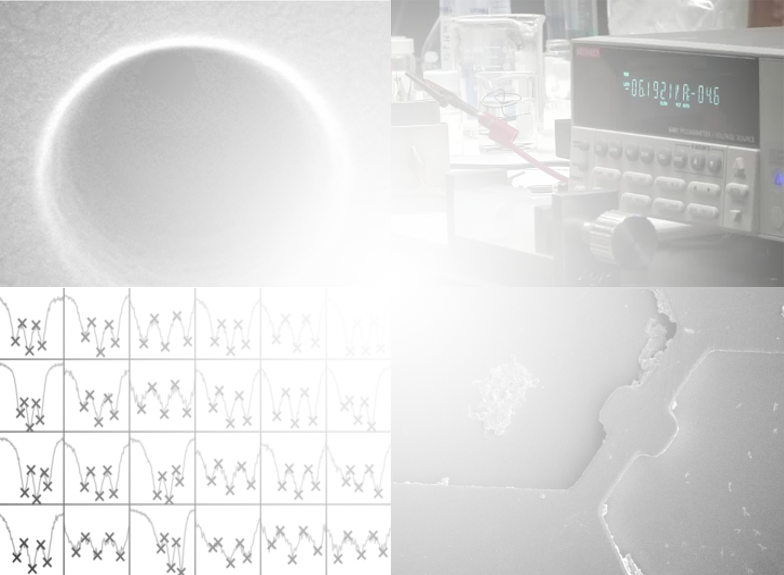
\includegraphics[width=\paperwidth,height=\paperheight]{title_image.png}}}
\begin{frame}[c]
 \begin{center}
  

  
  % Title
  \Huge{
	\textcolor{gray0}{Resistive Pulse Sensing at the Micro- and Nanoscale}
  }
  
  
  % Name --- Institution
  \vspace{.25in}
  {\Large 
	\textcolor{gray1}{Preston Hinkle} \hspace{.5in} 
\includegraphics[height=1em]{uci_wordmark.png}
  }
  
  
  % Talk location
  \vspace{.5in}
  {\small
	\textit{\today}
  }
  
  
  
 \end{center}

\end{frame}
}



%%%%%%%%%%%%%%%%%%%%%%%%%%%%%%%%%%%%%%%%%%%%%%%%%%%%%%%%%%%%%%%%%%%%%%%%%%%%%%%%%%%%%%%%%%%%%%%%%%%%%%%%%%%%%%%%%%%%%%%%%%%%
% Outline
%%%%%%%%%%%%%%%%%%%%%%%%%%%%%%%%%%%%%%%%%%%%%%%%%%%%%%%%%%%%%%%%%%%%%%%%%%%%%%%%%%%%%%%%%%%%%%%%%%%%%%%%%%%%%%%%%%%%%%%%%%%%


\begin{frame}[c]{Outline}
 
	\begin{columns}[t]
		\begin{column}[T]{2.25in}
		
			\setbeamercovered{transparent}
			\begin{itemize}
				\item\only<1>{\textcolor{porestatsblack}{Resistive pulse sensing background}}\only<2,3,4>{\textcolor{ucigray0}{Resistive pulse sensing background}}
				\item\only<2>{\textcolor{porestatsblack}{Resistive pulse sensing of high-aspect ratio particles}}\only<1,3,4>{\textcolor{ucigray0}{Resistive pulse sensing of high-aspect ratio particles}}	
				\item\only<3,4>{\textcolor{porestatsblack}{Microscale resistive pulse sensing}}\only<1,2>{\textcolor{ucigray0}{Microscale resistive pulse sensing}}
				
					\begin{itemize}
						\item\only<3>{\textcolor{porestatsblack}{Simultaneous imaging and resistive pulse studies}}\only<1,2,4>{\textcolor{ucigray0}{Simultaneous imaging and resistive pulse studies}}
						\item\only<4>{\textcolor{porestatsblack}{Cancer cell deformability cytometry}}\only<1,2,3>{\textcolor{ucigray0}{Cancer cell deformability cytometry}}
					\end{itemize}
					
					
				
			\end{itemize}
			\setbeamercovered{invisible}
			
		\end{column}
		
		
		\begin{column}[T]{2.25in}
	
		
			% RP Background 1
			\onslide<1>{
				\begin{picture}(0,0)(0,0)
					\put(35,-150)
					{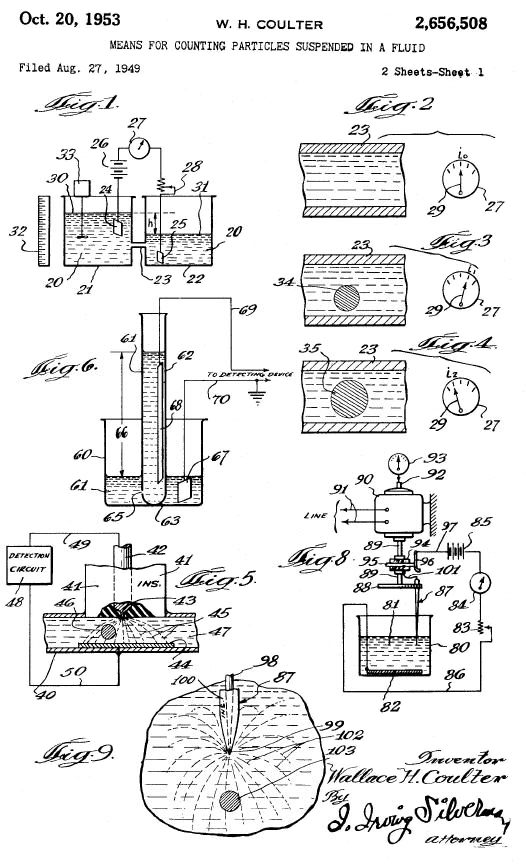
\includegraphics[width=1.5in]{coulter_patent_drawing}}
				\end{picture}
			}

		
			% Rods 1
			\onslide<2>{
				\begin{picture}(0,0)(0,0)
					\put(10,-30)
					{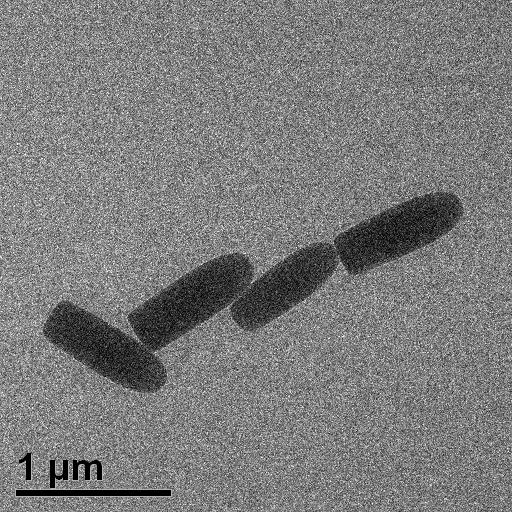
\includegraphics[width=1.25in]{shortrods}}
				\end{picture}
			}
			
			% Rods 2
			\onslide<2>{
				\begin{picture}(0,0)(0,0)
					\put(50,-125)
					{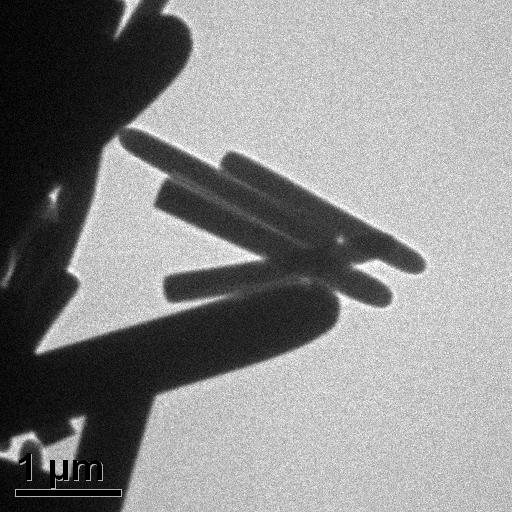
\includegraphics[width=1.25in]{longrods}}
				\end{picture}
			}
			
			
			% RPIM 1
			\onslide<3>{
				\begin{picture}(0,0)(0,0)
					\put(0, -65)
					{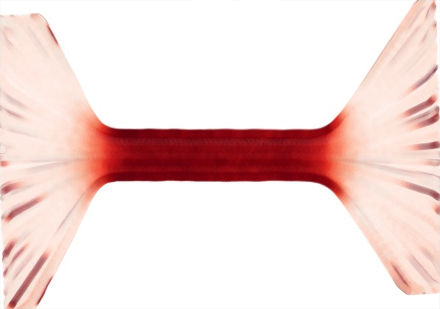
\includegraphics[width=2.25in]{resistancemap}}
				\end{picture}
			}
			
			% Cells
			\onslide<4>{
				\begin{picture}(0,0)(0,0)
					\put(0, -75)
					{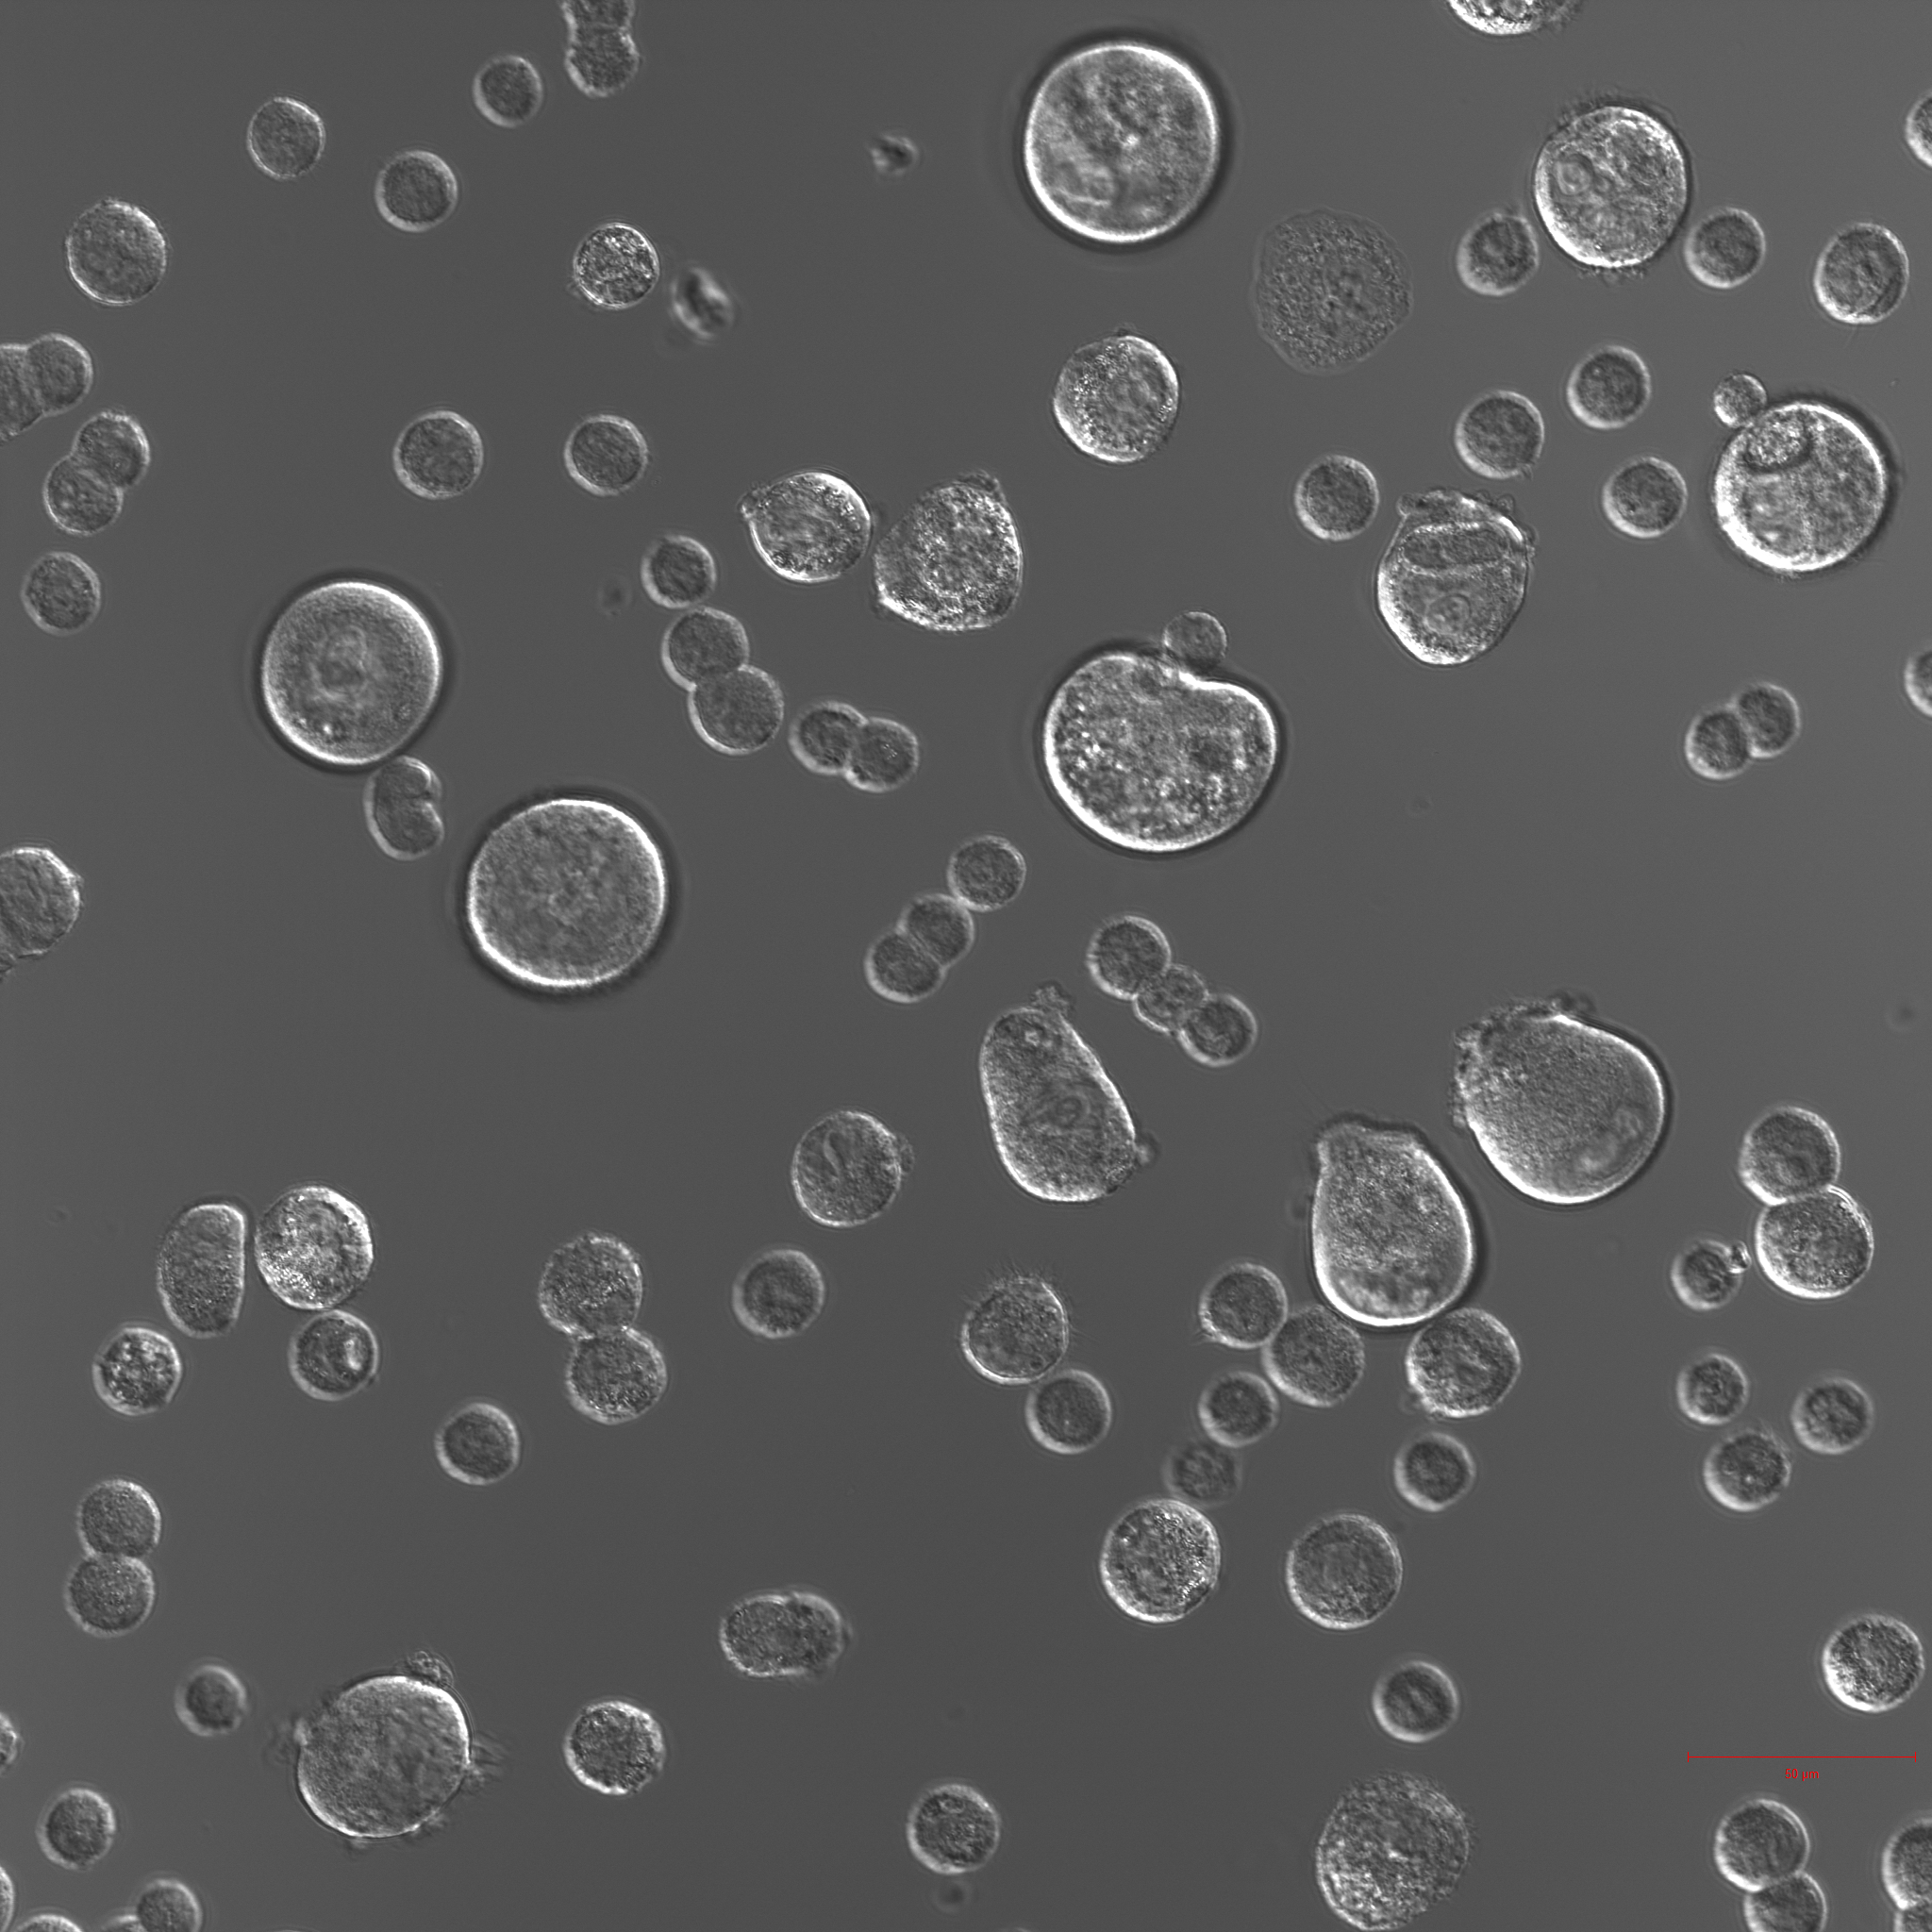
\includegraphics[width=2.25in]{cells}}
				\end{picture}
			}


			
			
		\end{column}
		
	\end{columns}

	
	
	
	
	
\end{frame}


%%%%%%%%%%%%%%%%%%%%%%%%%%%%%%%%%%%%%%%%%%%%%%%%%%%%%%%%%%%%%%%%%%%%%%%%%%%%%%%%%%%%%%%%%%%%%%%%%%%%%%%%%%%%%%%%%%%%%%%%%%%%
% Resistive pulse background title slide
%%%%%%%%%%%%%%%%%%%%%%%%%%%%%%%%%%%%%%%%%%%%%%%%%%%%%%%%%%%%%%%%%%%%%%%%%%%%%%%%%%%%%%%%%%%%%%%%%%%%%%%%%%%%%%%%%%%%%%%%%%%%


\begin{frame}[c]{}
	\begin{center}
		\textbf{Resistive pulse sensing background}
	\end{center}
\end{frame}



%%%%%%%%%%%%%%%%%%%%%%%%%%%%%%%%%%%%%%%%%%%%%%%%%%%%%%%%%%%%%%%%%%%%%%%%%%%%%%%%%%%%%%%%%%%%%%%%%%%%%%%%%%%%%%%%%%%%%%%%%%%%
% Resistive pulse background---description
%%%%%%%%%%%%%%%%%%%%%%%%%%%%%%%%%%%%%%%%%%%%%%%%%%%%%%%%%%%%%%%%%%%%%%%%%%%%%%%%%%%%%%%%%%%%%%%%%%%%%%%%%%%%%%%%%%%%%%%%%%%%


\begin{frame}[c]{Resistive pulse sensing---description}
	
	
	
			\begin{itemize}
				\item Resistive pulse sensing (RP) is a method for single particle detection and characterization
				\item Works at any scale (nano, micro, milli, etc.) and in a diverse range of applications
			\end{itemize}
	

	\begin{columns}[t]
		\begin{column}[T]{1.67in}
			{\centering
				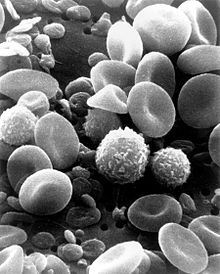
\includegraphics[height=1.25in]{bloodcells.jpg} \\
				Blood cell counting \\
				$\left(\sim\mathrm{several}\,\SI{}{\mu m}\right)$ \\
				\par
			}
		\end{column}
		
		\begin{column}[T]{1.67in}
			{\centering
				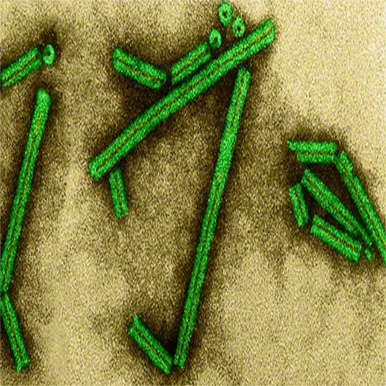
\includegraphics[height=1.25in]{tobaccomosaicvirus.png} \\
				Virus detection \\
				$\left(\sim\SI{50}{nm}\right)$ \\
				\par
			}
		\end{column}
		
		\begin{column}[T]{1.67in}
			{\centering
				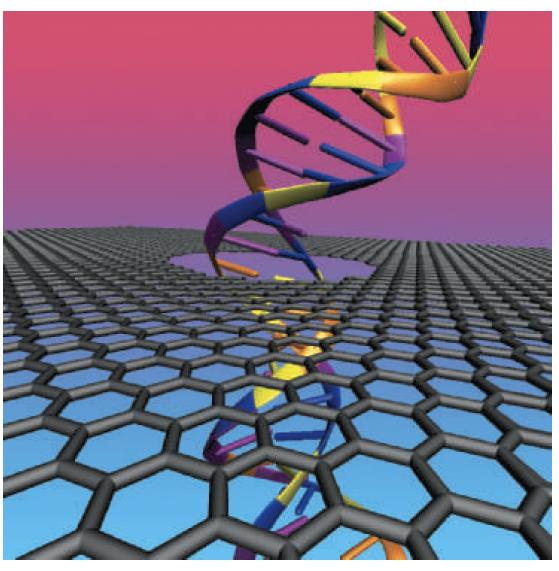
\includegraphics[height=1.25in]{dna.png} \\
				DNA sequencing \\
				$\left(\SI{1}{nm}\right)$ \\
				\par
			}
		\end{column}

	\end{columns}

	
\end{frame}



%%%%%%%%%%%%%%%%%%%%%%%%%%%%%%%%%%%%%%%%%%%%%%%%%%%%%%%%%%%%%%%%%%%%%%%%%%%%%%%%%%%%%%%%%%%%%%%%%%%%%%%%%%%%%%%%%%%%%%%%%%%%
% Resistive pulse background---how does it work?
%%%%%%%%%%%%%%%%%%%%%%%%%%%%%%%%%%%%%%%%%%%%%%%%%%%%%%%%%%%%%%%%%%%%%%%%%%%%%%%%%%%%%%%%%%%%%%%%%%%%%%%%%%%%%%%%%%%%%%%%%%%%


\begin{frame}[c]{Resistive pulse sensing---how does it work?}

	\begin{itemize}
		\item A channel is immersed in electrolyte solution
		\item An applied voltage induces an ionic current according to Ohm's law $I=V/R$
		\item The channel's resistance $R$ is a function of the channel geometry and the conductivity of solution it is filled with
	\end{itemize}


	{\centering 
		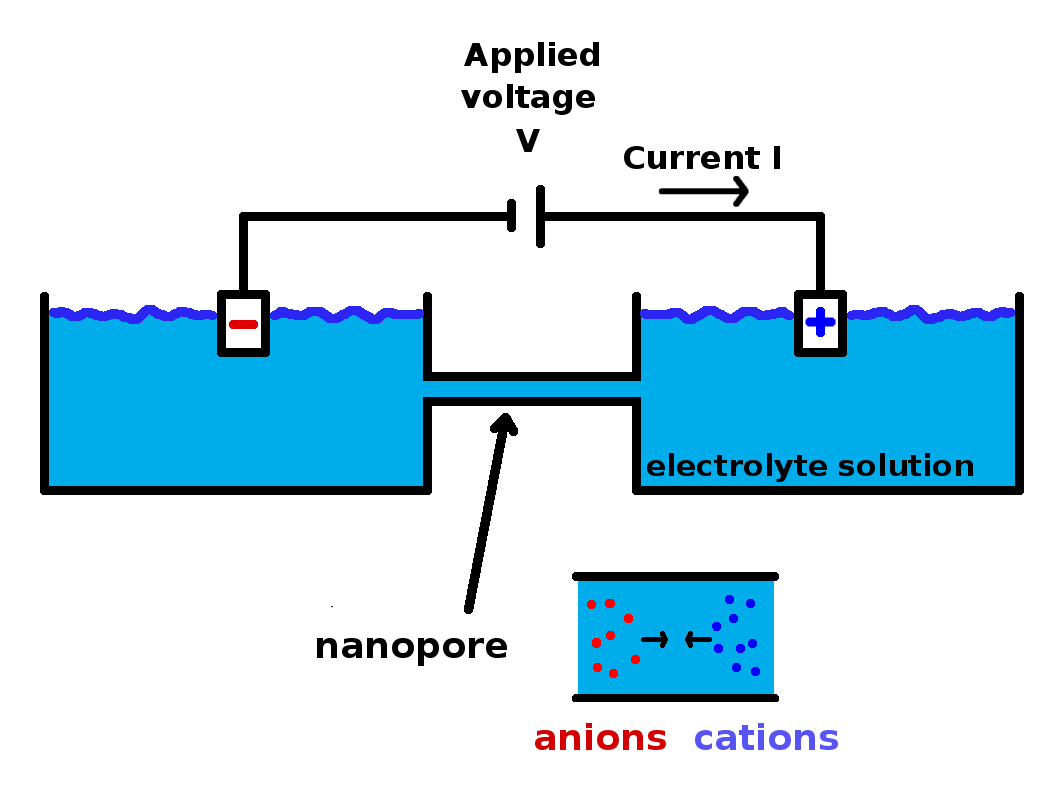
\includegraphics[width=2.5in]{nanopore_cartoon.png} \\
		\par
	}

	
\end{frame}


%%%%%%%%%%%%%%%%%%%%%%%%%%%%%%%%%%%%%%%%%%%%%%%%%%%%%%%%%%%%%%%%%%%%%%%%%%%%%%%%%%%%%%%%%%%%%%%%%%%%%%%%%%%%%%%%%%%%%%%%%%%%
% Resistive pulse background---how does it work?
%%%%%%%%%%%%%%%%%%%%%%%%%%%%%%%%%%%%%%%%%%%%%%%%%%%%%%%%%%%%%%%%%%%%%%%%%%%%%%%%%%%%%%%%%%%%%%%%%%%%%%%%%%%%%%%%%%%%%%%%%%%%

\begin{frame}[c]{Resistive pulse sensing---how does it work?}

	\begin{itemize}
		\item When a particle enters the channel, the channel's resistance changes, yielding a pulse in the measured ionic current
		\item Pulse properties yield information on size, shape, charge, and concentration of particle
	\end{itemize}
	
	\begin{columns}[t]
	
		\begin{column}[T]{2.25in}
			{\centering
				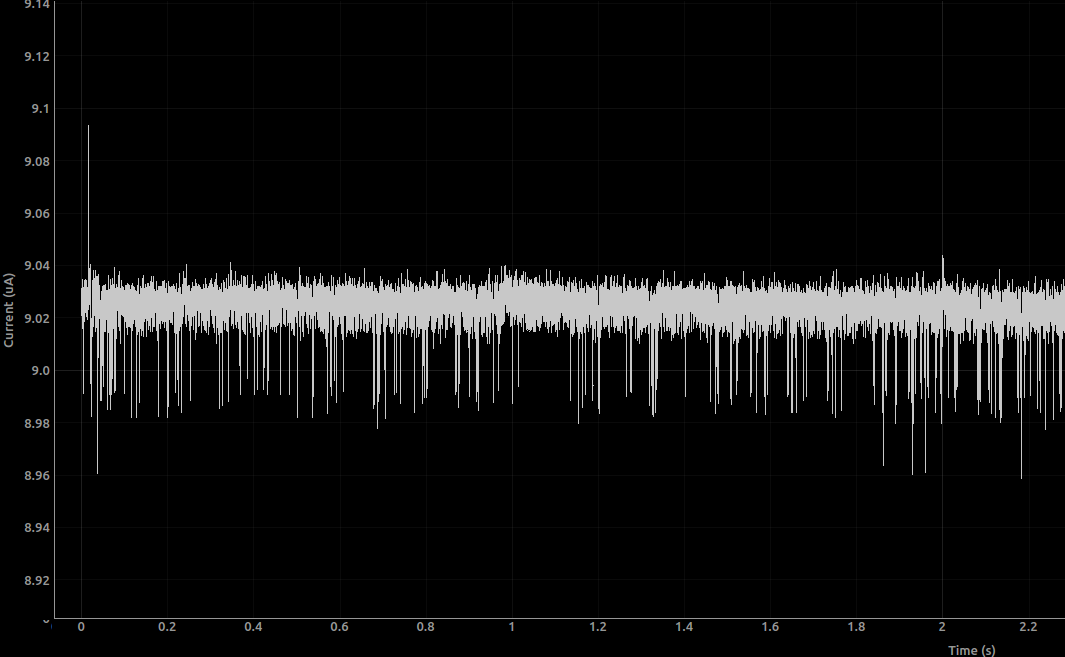
\includegraphics[height=1.25in]{rp_timeseries.png} \\
				Resistive pulse time series \\
				\par
			}
		\end{column}
		
		\begin{column}[T]{2.25in}
			{\centering
				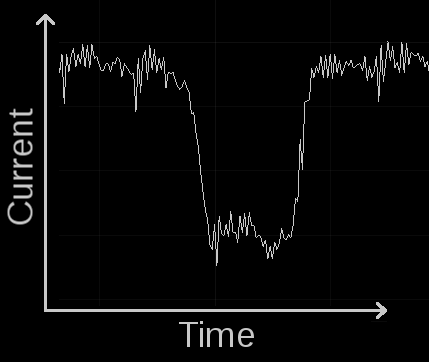
\includegraphics[height=1.25in]{singlerp} \\
				Series zoomed in on a single event \\
				\par
			}
		\end{column}

	\end{columns}


	
\end{frame}


		


%%%%%%%%%%%%%%%%%%%%%%%%%%%%%%%%%%%%%%%%%%%%%%%%%%%%%%%%%%%%%%%%%%%%%%%%%%%%%%%%%%%%%%%%%%%%%%%%%%%%%%%%%%%%%%%%%%%%%%%%%%%%
% Resistive pulse background---physics
%%%%%%%%%%%%%%%%%%%%%%%%%%%%%%%%%%%%%%%%%%%%%%%%%%%%%%%%%%%%%%%%%%%%%%%%%%%%%%%%%%%%%%%%%%%%%%%%%%%%%%%%%%%%%%%%%%%%%%%%%%%%

\begin{frame}[c]{Resistive pulse sensing---physics}

	In order to understand resistive pulse sensing and the amplitudes of the event pulses, we need to consider the following domains of physics
	
	\begin{itemize}
		\item Ion transport mechanisms
		\item Electrodynamics
		\item Particle transport mechanisms
	\end{itemize}

\end{frame}


%%%%%%%%%%%%%%%%%%%%%%%%%%%%%%%%%%%%%%%%%%%%%%%%%%%%%%%%%%%%%%%%%%%%%%%%%%%%%%%%%%%%%%%%%%%%%%%%%%%%%%%%%%%%%%%%%%%%%%%%%%%%
% Resistive pulse background---ion transport
%%%%%%%%%%%%%%%%%%%%%%%%%%%%%%%%%%%%%%%%%%%%%%%%%%%%%%%%%%%%%%%%%%%%%%%%%%%%%%%%%%%%%%%%%%%%%%%%%%%%%%%%%%%%%%%%%%%%%%%%%%%%

\tikzset{cross/.style={cross out, draw=black, minimum size=2*(#1-\pgflinewidth), inner sep=0pt, outer sep=0pt},
%default radius will be 1pt. 
cross/.default={1pt}}



\begin{frame}[c]{Resistive pulse sensing---ion transport}	
	\begin{itemize}
		\item Ion transport in general occurs via a combination of \textbf{diffusion}, \textbf{convection}, and \textbf{electrophoresis} (or electrophoresis)
		\item \underline{Diffusion}: Average flow of ions from high to low concentration
		\item \underline{Convection}: Ions are carried passively with the fluid/solvent
		\item \underline{Electrophoresis}: Ions drift in an electric field
	\end{itemize}
	\only<1>{
		\begin{equation} \tag{Nernst-Planck equation}
			\vec{J}=\sum_{i}^{\mathrm{species}}\left[\underbrace{-z_{i}eD_{i}\nabla c_{i}}_{\mathrm{diffusion}} + \overbrace{z_{i}ec_{i}\vec{u}}^{\mathrm{convection}}+\underbrace{z_{i}ec_{i}\mu^{ep}_{i}\vec{E}}_{\mathrm{electrophoresis}}\right]
		\end{equation}
	}\only<2>{
		\begin{equation} \tag{Nernst-Planck equation}
			\vec{J}=\sum_{i}^{\mathrm{species}}\left[\underbrace{\xcancel{-z_{i}eD_{i}\nabla c_{i}}}_{\mathrm{diffusion}} + \overbrace{\xcancel{z_{i}ec_{i}\vec{u}}}^{\mathrm{convection}}+\underbrace{z_{i}ec_{i}\mu^{ep}_{i}\vec{E}}_{\mathrm{migration}}\right]
		\end{equation}
	}
	\only<3>{
		\begin{equation} \tag{Electrophoretic current}
			\vec{J}=\sum_{i}^{\mathrm{species}}z_{i}ec_{i}\mu^{ep}_{i}\vec{E}=\sigma\vec{E}
		\end{equation}
	}
	\begin{equation} \tag{Einstein-Smoluchowski relation} 
		\mu^{ep}_{i}=\frac{z_{i}e}{k_{B}T}D_{i}
	\end{equation}

	


\end{frame}


%%%%%%%%%%%%%%%%%%%%%%%%%%%%%%%%%%%%%%%%%%%%%%%%%%%%%%%%%%%%%%%%%%%%%%%%%%%%%%%%%%%%%%%%%%%%%%%%%%%%%%%%%%%%%%%%%%%%%%%%%%%%
% Resistive pulse background---electrostatics
%%%%%%%%%%%%%%%%%%%%%%%%%%%%%%%%%%%%%%%%%%%%%%%%%%%%%%%%%%%%%%%%%%%%%%%%%%%%%%%%%%%%%%%%%%%%%%%%%%%%%%%%%%%%%%%%%%%%%%%%%%%%

\begin{frame}[c]{Resistive pulse sensing---electrodynamics}

	To solve for the currents in the pore (empty and occupied), we treat the system as a classical electrodynamics problem \\
		\begin{align}		
			\vec{J} &= \sigma\vec{E} \tag{Ohm's law} \\
			\rightarrow \nabla^{2}V &= 0 \tag{Laplace equation} \\
			\left. \vec{J}\cdot\hat{n}\right\vert_{\mathrm{channel}} &= 0 \tag{Boundary conditions}\\
			\left. \vec{J}\cdot\hat{t}\right\vert_{\mathrm{electrode}} &= 0 \notag
		\end{align}
		
	For an unoccupied cylindrical pore with electrodes exactly at the pore entrance and exit, we find
	
	\begin{equation} \tag{Ideal cylinder}
		R=\rho\frac{L}{A}
	\end{equation}
	

\end{frame}



%%%%%%%%%%%%%%%%%%%%%%%%%%%%%%%%%%%%%%%%%%%%%%%%%%%%%%%%%%%%%%%%%%%%%%%%%%%%%%%%%%%%%%%%%%%%%%%%%%%%%%%%%%%%%%%%%%%%%%%%%%%%
% Resistive pulse background---electrostatics
%%%%%%%%%%%%%%%%%%%%%%%%%%%%%%%%%%%%%%%%%%%%%%%%%%%%%%%%%%%%%%%%%%%%%%%%%%%%%%%%%%%%%%%%%%%%%%%%%%%%%%%%%%%%%%%%%%%%%%%%%%%%

\begin{frame}[c]{Resistive pulse sensing---electrodynamics}


		The presence of an insulating particle increases the system resistance for two reasons
		
		\begin{enumerate}
			\item The volume occupied by the particle no longer contains conductive solution
			\item Electric field lines in the vicinity of the particle are distorted, with reduced axial components
		\end{enumerate}
		
		The result is a \underline{decrease in current} when the particle is inside the channel
		
		{\centering
			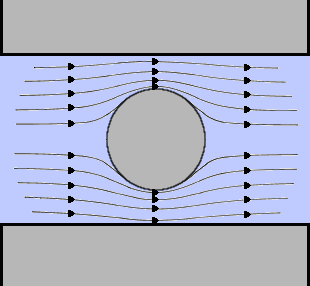
\includegraphics[width=1.5in]{efield.png} \\
			\par
		}
		

\end{frame}



%%%%%%%%%%%%%%%%%%%%%%%%%%%%%%%%%%%%%%%%%%%%%%%%%%%%%%%%%%%%%%%%%%%%%%%%%%%%%%%%%%%%%%%%%%%%%%%%%%%%%%%%%%%%%%%%%%%%%%%%%%%%
% Resistive pulse background---electrostatics
%%%%%%%%%%%%%%%%%%%%%%%%%%%%%%%%%%%%%%%%%%%%%%%%%%%%%%%%%%%%%%%%%%%%%%%%%%%%%%%%%%%%%%%%%%%%%%%%%%%%%%%%%%%%%%%%%%%%%%%%%%%%

\begin{frame}[c]{Resistive pulse sensing---electrodynamics}
 
	Ignoring the distortion of the electric field, a reasonable approximation for the resistance of the channel with or without the particle can be found \textit{via}
		
	\[ \Delta R=\int\rho\frac{dz}{A\left(z\right)} \],
		
	where $A\left(z\right)$ is area of the annular region of solution at position $z$

\end{frame}


%%%%%%%%%%%%%%%%%%%%%%%%%%%%%%%%%%%%%%%%%%%%%%%%%%%%%%%%%%%%%%%%%%%%%%%%%%%%%%%%%%%%%%%%%%%%%%%%%%%%%%%%%%%%%%%%%%%%%%%%%%%%
% Resistive pulse background---electrostatics
%%%%%%%%%%%%%%%%%%%%%%%%%%%%%%%%%%%%%%%%%%%%%%%%%%%%%%%%%%%%%%%%%%%%%%%%%%%%%%%%%%%%%%%%%%%%%%%%%%%%%%%%%%%%%%%%%%%%%%%%%%%%

\begin{frame}[c]{Resistive pulse sensing---electrodynamics}

		% Clarify symbols and spend less time on the explanatoin


		Analytic solutions to resistive pulse amplitude:
		\vspace{.1in}
		
		\begin{columns}[t]
			\begin{column}[T]{2.5in}
				\begin{equation} \tag{Sphere through cylinder}
					\frac{\Delta R}{R_{0}}=\frac{3}{2}\frac{v}{V}
				\end{equation}
				\vspace{-.1in}				
				\begin{equation} \tag{Ellipsoid through cylinder}
					\frac{\Delta R}{R_{0}}=\left[f_{\perp}+\left(f_{\parallel}-f_{\perp}\right)\cos^{2}\alpha\right]\frac{v}{V}
				\end{equation}
			\end{column}
			\hfill
			\begin{column}[T]{1.5in}
				$v$: Particle diameter \\
				\vspace{.0675in}
				$V$: Channel diameter \\
				\vspace{.0675in}
				$f_{\perp}, f_{\parallel}$: Electrical shape factors \\
				\vspace{.0675in}
				$\alpha$: Angle of rotation
			\end{column}

		\end{columns}

		
		\vspace{0.1in}
		{\centering
			\noindent\rule{4.5in}{1pt} \\
			\par
		}

		
		Since we usually measure current in an experiment instead of resistance, it's conventional to replace $R$ for $I$ using Ohm's law:
		\[ \frac{\Delta R}{R_{0}}\Rightarrow\frac{\Delta I}{I_{p}} \]
\end{frame}






%%%%%%%%%%%%%%%%%%%%%%%%%%%%%%%%%%%%%%%%%%%%%%%%%%%%%%%%%%%%%%%%%%%%%%%%%%%%%%%%%%%%%%%%%%%%%%%%%%%%%%%%%%%%%%%%%%%%%%%%%%%%
% Resistive pulse background---particle transport
%%%%%%%%%%%%%%%%%%%%%%%%%%%%%%%%%%%%%%%%%%%%%%%%%%%%%%%%%%%%%%%%%%%%%%%%%%%%%%%%%%%%%%%%%%%%%%%%%%%%%%%%%%%%%%%%%%%%%%%%%%%%

\begin{frame}[c]{Resistive pulse sensing---single particle transport}
	Similar to ions, single particle transport can occur via \textbf{thermal motion}, \textbf{convection}, and \textbf{electrophoresis}
	\begin{itemize}
		\item \underline{Thermal motion}: Collisions with atoms and molecules causes random diffusive motion
		\item \underline{Convection}: Motion due to fluid flow, usually induced by external pressure or electroosmosis
		\item \underline{Electrophoresis}: Effective force on charged particles in electric fields
	\end{itemize}
	
	
	%$$ \vec{u}=\mu_{EP}\vec{E}+\mu_{EO}

\end{frame}



%%%%%%%%%%%%%%%%%%%%%%%%%%%%%%%%%%%%%%%%%%%%%%%%%%%%%%%%%%%%%%%%%%%%%%%%%%%%%%%%%%%%%%%%%%%%%%%%%%%%%%%%%%%%%%%%%%%%%%%%%%%%
% Rods title slide
%%%%%%%%%%%%%%%%%%%%%%%%%%%%%%%%%%%%%%%%%%%%%%%%%%%%%%%%%%%%%%%%%%%%%%%%%%%%%%%%%%%%%%%%%%%%%%%%%%%%%%%%%%%%%%%%%%%%%%%%%%%%


\begin{frame}[c]{}
	\begin{center}
		\textbf{Resistive pulse sensing of high-aspect ratio particles}
	\end{center}
\end{frame}




%%%%%%%%%%%%%%%%%%%%%%%%%%%%%%%%%%%%%%%%%%%%%%%%%%%%%%%%%%%%%%%%%%%%%%%%%%%%%%%%%%%%%%%%%%%%%%%%%%%%%%%%%%%%%%%%%%%%%%%%%%%%
% Rods motivation slide
%%%%%%%%%%%%%%%%%%%%%%%%%%%%%%%%%%%%%%%%%%%%%%%%%%%%%%%%%%%%%%%%%%%%%%%%%%%%%%%%%%%%%%%%%%%%%%%%%%%%%%%%%%%%%%%%%%%%%%%%%%%%


\begin{frame}[c]{High-aspect ratio resistive pulse sensing---motivation}
 	
 	% Keep in back pocket idea about the fact that particle shape is related to time it spends in blood stream; important for drug delivery systems.
 	
 	\begin{itemize}
 		\item Aspherical particles are ubiquitous in biology---e.g., many viruses and bacteria are approximately ellipsoidal
 	\end{itemize}


	\begin{columns}[t]
		\begin{column}[T]{2.5in}
			{\centering
				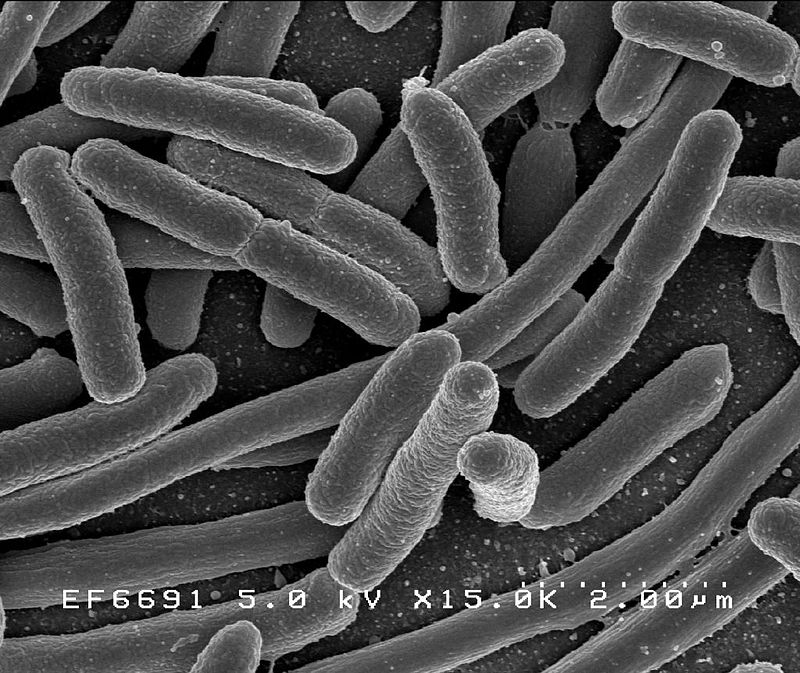
\includegraphics[height=2.25cm]{ecoli} \\
				e. coli \\
				$L\sim \SI{2}{\mu m}$ \\
				\par
			}
		\end{column}
		
		
		\begin{column}[T]{2.5in}
			{\centering
				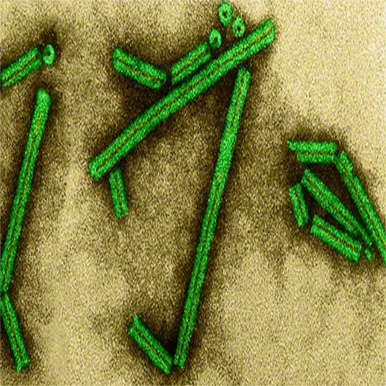
\includegraphics[height=2.25cm]{tobaccomosaicvirus} \\
				tobacco mosaic virus \\
				$L\sim \SI{300}{nm}$ \\
				\par
			}
		\end{column}
	

	\end{columns}

	\begin{itemize}
		\item The ability to measure particle shape is highly desirable for sensing applications
 		\item How an we extend RP sensing to measure length in addition to volume?
 	\end{itemize}
	

\end{frame}




%%%%%%%%%%%%%%%%%%%%%%%%%%%%%%%%%%%%%%%%%%%%%%%%%%%%%%%%%%%%%%%%%%%%%%%%%%%%%%%%%%%%%%%%%%%%%%%%%%%%%%%%%%%%%%%%%%%%%%%%%%%%
% Resistive pulse in non-constant width pores
%%%%%%%%%%%%%%%%%%%%%%%%%%%%%%%%%%%%%%%%%%%%%%%%%%%%%%%%%%%%%%%%%%%%%%%%%%%%%%%%%%%%%%%%%%%%%%%%%%%%%%%%%%%%%%%%%%%%%%%%%%%%

\begin{frame}[c]{Resistive pulse in non-uniform pores}

	{\small Consider the RP amplitude for translocation through non-uniform pores} \\
	{\small
		$$ \Delta R\left(z'\right)=\frac{\rho}{\pi}\left[\int_{z=z'}^{z=z'+l_{p}}\left(\frac{1}{r_{P}^{2}\left(z\right)-s_{p}^{2}\left(z\right)}-\frac{1}{r_{P}\left(z\right)^{2}}\right)dz\right] $$
	}
	
	\vspace{.1in}
	
	\begin{columns}[t]
		\begin{column}[T]{2.5in}
			{\small
				RP amplitude is a function of the pore geometry \textbf{local to the particle's position} \\
				\vspace{.2in}
				Particles map the interior of the pore during translocation with their RP signal! \\
			}
		\end{column}
		
		\begin{column}[T]{2in}
			{\centering
				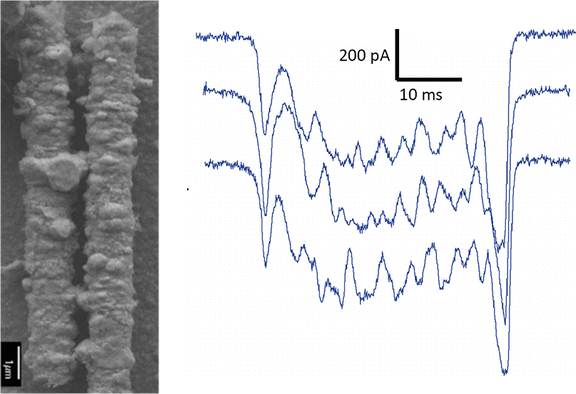
\includegraphics[width=2in]{particlesreveal.png} \\
				{\tiny Pevarnik \textit{et al}. \textit{ACS Nano.} \textbf{6}, 7295-7302 (2012).} \\
				\par
			}
		\end{column}
	\end{columns}

	
	
	
	

	
\end{frame}


%%%%%%%%%%%%%%%%%%%%%%%%%%%%%%%%%%%%%%%%%%%%%%%%%%%%%%%%%%%%%%%%%%%%%%%%%%%%%%%%%%%%%%%%%%%%%%%%%%%%%%%%%%%%%%%%%%%%%%%%%%%%
% RP signal resolution
%%%%%%%%%%%%%%%%%%%%%%%%%%%%%%%%%%%%%%%%%%%%%%%%%%%%%%%%%%%%%%%%%%%%%%%%%%%%%%%%%%%%%%%%%%%%%%%%%%%%%%%%%%%%%%%%%%%%%%%%%%%%

\begin{frame}[c]{RP signal resolution}
	
	\vspace{-.1in}
	\begin{itemize}
		\item Particles map pore interiors with a length-dependent resolution
		\item If a particle has length less than the characteristic length scale of channel irregularities, the produced signal is a high-resolution mapping
		\item Particles with lengths greater than characteristic length scale of channel irregularities produce low-resolution mappings
	\end{itemize}
	
	
	
	\begin{columns}[t]
		
	
		\begin{column}[T]{2.25in}
			{\centering
				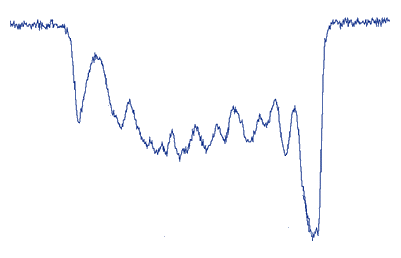
\includegraphics[height=1in]{plain_signal.png} \\
				Short particle \\
			}
		\end{column}
		  
		\begin{column}[T]{2.25in}
			{\centering
				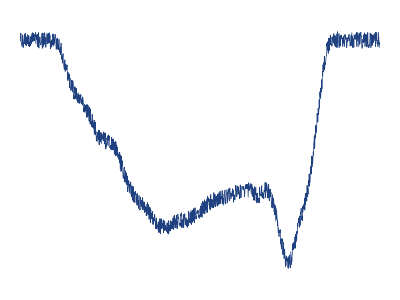
\includegraphics[height=1.in,width=2in]{mystery_plain_signal_3.png} \\
				Long particle (simulated) \\
			}
		\end{column}

	\end{columns}
	\vspace{.2in}
	{\large \textcolor{negativered}{Can we use this knowledge to measure particle length?}}

	%$$ \Delta R\left(z'\right)=\frac{\rho}{\pi}\left[\int_{z=z'}^{z=z'+l_{p}}\left(\frac{1}{r_{P}^{2}\left(z\right)-s_{p}^{2}\left(z\right)}-\frac{1}{r_{P}^{2}\left(z\right)}\right)dz\right] $$

	
	
	
	

\end{frame}


%%%%%%%%%%%%%%%%%%%%%%%%%%%%%%%%%%%%%%%%%%%%%%%%%%%%%%%%%%%%%%%%%%%%%%%%%%%%%%%%%%%%%%%%%%%%%%%%%%%%%%%%%%%%%%%%%%%%%%%%%%%%
% Qualitative length comparison
%%%%%%%%%%%%%%%%%%%%%%%%%%%%%%%%%%%%%%%%%%%%%%%%%%%%%%%%%%%%%%%%%%%%%%%%%%%%%%%%%%%%%%%%%%%%%%%%%%%%%%%%%%%%%%%%%%%%%%%%%%%%

\begin{frame}[c]{Qualitative length comparison}
	\vspace{.3in}
	\begin{picture}(0,0)(0,0)
		\put(0,-25)
		{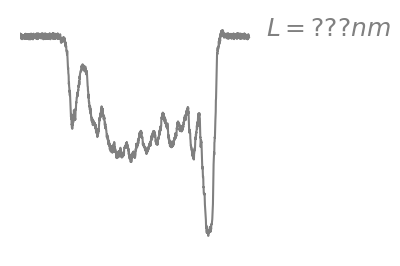
\includegraphics[width=3.75cm]{mystery_plain_signal_2.png}}
		\put(0,-125)
		{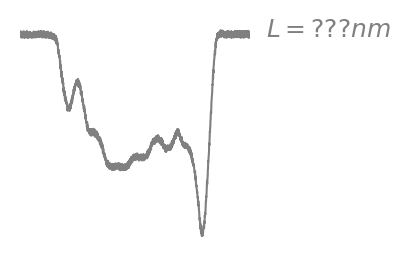
\includegraphics[width=3.75cm]{mystery_plain_signal.png}}
		\put(200,-125)
		{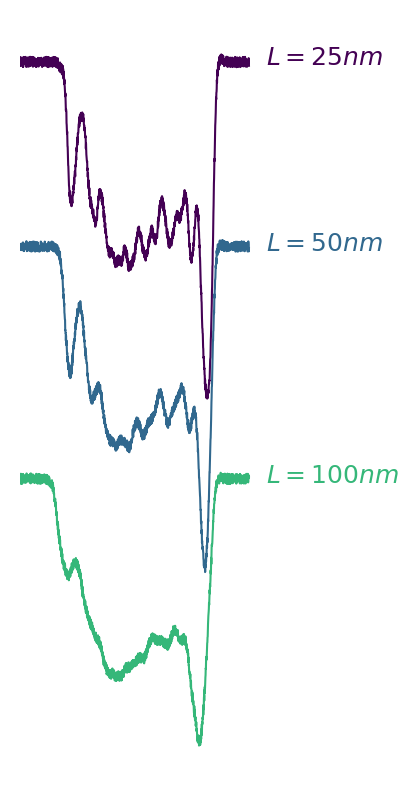
\includegraphics[height=7cm]{plain_signals_smoothed.png}}
	\end{picture}
	
	\begin{tikzpicture}[overlay, x=1cm,y=1cm]
		% Coordinates
		\coordinate (x1) at (2.5, -2.5) ;
		\coordinate (x2) at (5.5, -2.5) ;
		\coordinate (x3) at (5.5, -.5) ;
		\coordinate (x4) at (7.25, -.5) ;
		
		
		\coordinate (x5) at (2.5, 1.) ;
		\coordinate (x6) at (5.5, 1.) ;
		\coordinate (x7) at (5.5, 2.95) ;
		\coordinate (x8) at (7.25, 2.95) ;

		% Text hack
		\node[right] (mag) at (0.25,3.5) {\footnotesize\textcolor{porestatsblack}{Unidentified particles}};
		\node[right] (mag) at (7.25,3.5) {\footnotesize\textcolor{porestatsblack}{Tracer particles}};


		    		    
		% Arrow
		\path[draw=gray1,thick,->] (x1) to[straight] (x2) to[straight] (x3) to[straight] (x4);
		\path[draw=gray1,thick,->] (x5) to[straight] (x6) to[straight] (x7) to[straight] (x8);


			
	\end{tikzpicture}
	

\end{frame}


%%%%%%%%%%%%%%%%%%%%%%%%%%%%%%%%%%%%%%%%%%%%%%%%%%%%%%%%%%%%%%%%%%%%%%%%%%%%%%%%%%%%%%%%%%%%%%%%%%%%%%%%%%%%%%%%%%%%%%%%%%%%
% Quantitative length measurement
%%%%%%%%%%%%%%%%%%%%%%%%%%%%%%%%%%%%%%%%%%%%%%%%%%%%%%%%%%%%%%%%%%%%%%%%%%%%%%%%%%%%%%%%%%%%%%%%%%%%%%%%%%%%%%%%%%%%%%%%%%%%

\begin{frame}[c]{Reexpressing the RP amplitude of a long particle in terms of shorter particles}
	
	
	{\footnotesize
	Because resistances add in series, we can express the RP amplitude of a long particle as a sum over the RP amplitudes of shorter particles
	}
	
	
	{\scriptsize
		\begin{equation*}
			\begin{split}
				\frac{\Delta I}{I_{p}}=\frac{\Delta R_{l}}{R_{0}} &= \frac{\rho}{\pi}\left[\int_{z}^{z+l_{p}}\left(\frac{1}{r_{P}^{2}\left(z'\right)-s_{p}^{2}\left(z'\right)}-\frac{1}{r_{P}^{2}\left(z'\right)}\right)dz'\right]/R_{0} \\
				%&= \frac{\rho}{\pi}\left[\int_{z}^{z+l_{s}}\left(\frac{1}{r_{P}^{2}\left(z'\right)-%s_{p}^{2}\left(z'\right)}-\frac{1}{r_{P}^{2}\left(z'\right)}\right)dz'\right. \\
				%&+ \int_{z+l_{s}}^{z+2l_{s}}\left(\frac{1}{r_{P}^{2}\left(z'\right)-s_{p}^{2}\left(z'\right)}-\frac{1}%{r_{P}^{2}\left(z'\right)}\right)dz + ...\\
				%&+ \left.\int_{z+\left(n-1\right)l_{s}}^{z+nl_{s}}\left(\frac{1}{r_{P}^{2}\left(z'\right)-%s_{p}^{2}\left(z'\right)}-\frac{1}{r_{P}^{2}\left(z'\right)}\right)dz'\right] \\
				&= \sum_{i=0}^{n-1}\frac{\rho}{\pi}\left[\int_{z+il_{s}}^{z+\left(i+1\right)l_{s}}\left(\frac{1}{r^{2}_{P}\left(z'\right)-s^{2}_{p}\left(z'\right)}-\frac{1}{r_{P}^{2}\left(z'\right)}\right)dz'\right]/R_{0} \\
				&= \sum_{i=0}^{n-1}\Delta R_{s}\left(z+il_{s}\right)/R_{0}
			\end{split}
		\end{equation*}
	}
	
		

\end{frame}




%%%%%%%%%%%%%%%%%%%%%%%%%%%%%%%%%%%%%%%%%%%%%%%%%%%%%%%%%%%%%%%%%%%%%%%%%%%%%%%%%%%%%%%%%%%%%%%%%%%%%%%%%%%%%%%%%%%%%%%%%%%%
% Quantitative length measurement
%%%%%%%%%%%%%%%%%%%%%%%%%%%%%%%%%%%%%%%%%%%%%%%%%%%%%%%%%%%%%%%%%%%%%%%%%%%%%%%%%%%%%%%%%%%%%%%%%%%%%%%%%%%%%%%%%%%%%%%%%%%%

\begin{frame}[c]{Quantitative length measurement}
	

	{\footnotesize
		Reexpressing the amplitude of long particles in terms of amplitude of short particles suggests a protocol for measuring length \\
		\begin{enumerate}
			\item We perform a moving average transformation on the signals of shorter particles to simulate the signals of longer particles \\
			%\[ S_{i}\rightarrow S'_{i}=\frac{1}{\Delta i}\sum_{i-\frac{\Delta i}{2}}^{i+\frac{\Delta I}{2}}S_{i} \]^{2}
			\item Then, we calculate the `distance' between an unknown particle's signal with each of the simulated signals of the shorter particle \\
			%\[ D\left(S^{\mathrm{long}},S'^{\mathrm{short}}\right)=\sum_{i,j}\left[S^{\mathrm{long}}_{i}-S'^{\mathrm{short}}_{j}\right] \]
			\item The comparison with the greatest similarity yields the length of the particle
		\end{enumerate}
	}
	


\end{frame}



%%%%%%%%%%%%%%%%%%%%%%%%%%%%%%%%%%%%%%%%%%%%%%%%%%%%%%%%%%%%%%%%%%%%%%%%%%%%%%%%%%%%%%%%%%%%%%%%%%%%%%%%%%%%%%%%%%%%%%%%%%%%
% Quantitative length measurement
%%%%%%%%%%%%%%%%%%%%%%%%%%%%%%%%%%%%%%%%%%%%%%%%%%%%%%%%%%%%%%%%%%%%%%%%%%%%%%%%%%%%%%%%%%%%%%%%%%%%%%%%%%%%%%%%%%%%%%%%%%%%

\begin{frame}[c]{Quantitative length measurement---parametric signal transformation}
	\begin{columns}[t]
	
		\begin{column}[T]{2.25in}
			{\centering
				Single transformation \\
				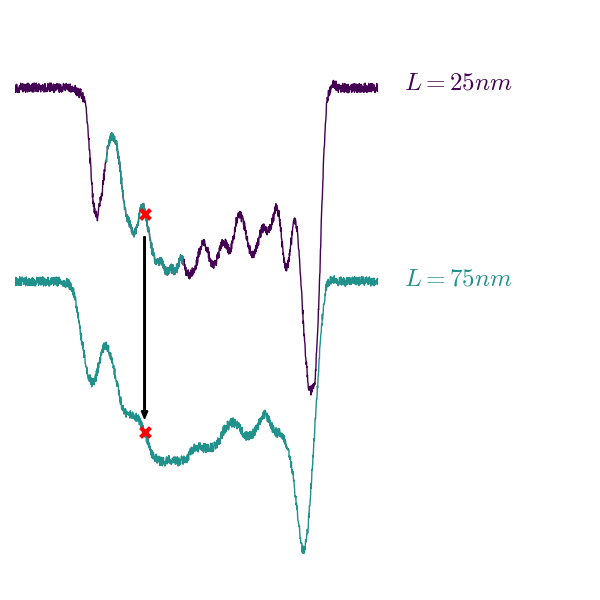
\includegraphics[width=2.25in]{moving_average_process.png} \\
				\par
			}
		\end{column}
		\hfill
		\begin{column}[T]{2.25in}
			{\centering
				Multiple length transformations \\
				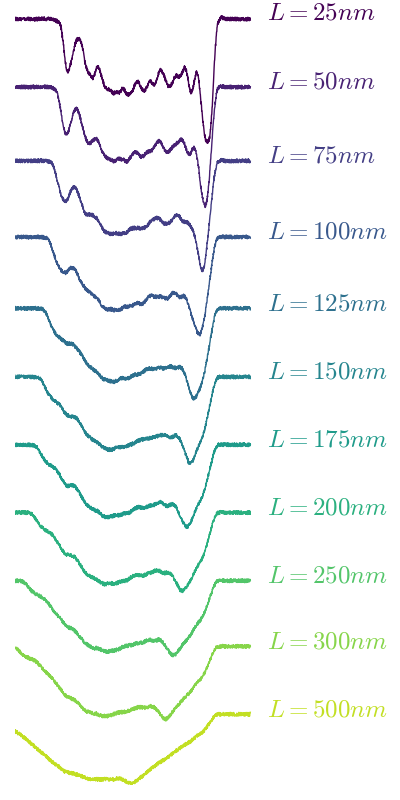
\includegraphics[width=1.25in]{many_plain_signals_smoothed.png} \\
				\par
			}
		\end{column}

	\end{columns}
	


\end{frame}



%%%%%%%%%%%%%%%%%%%%%%%%%%%%%%%%%%%%%%%%%%%%%%%%%%%%%%%%%%%%%%%%%%%%%%%%%%%%%%%%%%%%%%%%%%%%%%%%%%%%%%%%%%%%%%%%%%%%%%%%%%%%
% Quantitative length measurement
%%%%%%%%%%%%%%%%%%%%%%%%%%%%%%%%%%%%%%%%%%%%%%%%%%%%%%%%%%%%%%%%%%%%%%%%%%%%%%%%%%%%%%%%%%%%%%%%%%%%%%%%%%%%%%%%%%%%%%%%%%%%

\begin{frame}[c]{Quantitative length measurement---signal similarity measure}
	\vspace{-.1in}
	\begin{columns}[t]
	
		\begin{column}[T]{2.25in}
			{\centering
				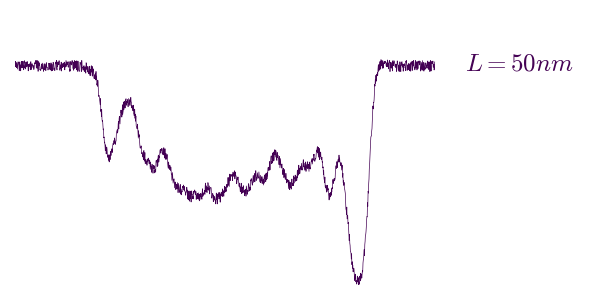
\includegraphics[width=2in]{mystery_signal_7.png} \\
				\par
			}
		\end{column}
		
		\begin{column}[T]{2.25in}
			{\centering
				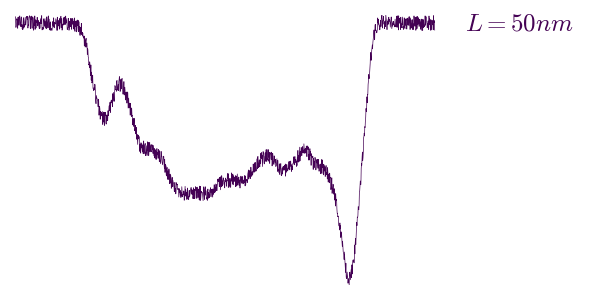
\includegraphics[width=2in]{transformed_signal.png} \\
				\par
			}
		\end{column}

	\end{columns}

	\vspace{.2in}	
	
	\begin{columns}[t]
	
		\begin{column}[T]{1.25in}
			{\centering
				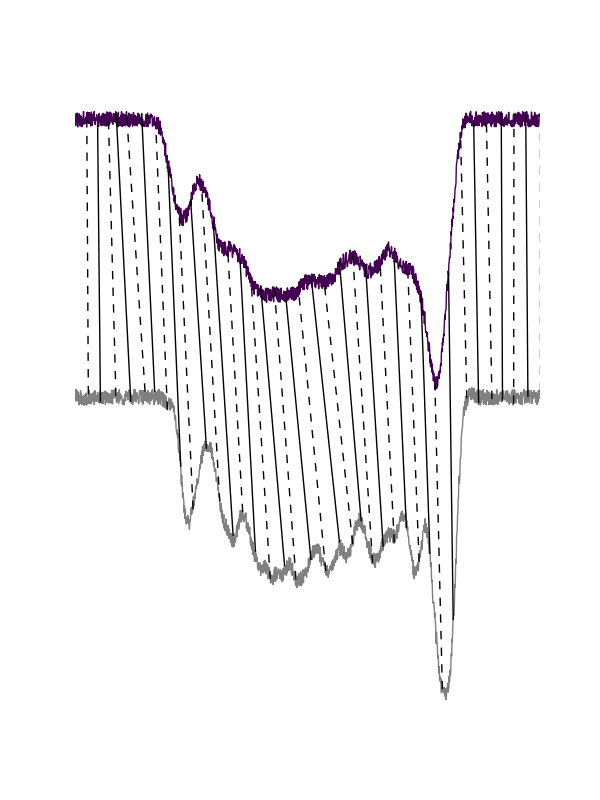
\includegraphics[width=1.25in]{dtw_matching.png} \\
				\par
			}
		\end{column}
		
		\begin{column}[T]{\paperwidth/3}
			{\centering
				\vspace{.2in}
				{\tiny \[\mathrm{Distance}=\sum_{\left(i,i'\right)}\left[\left(\frac{\Delta I}{I_{p}}\right)_{i}-\left(\frac{\Delta I}{I_{p}}\right)_{i'}\right]^{2} \] } \\
				\par
			}
		\end{column}
		
		\begin{column}[T]{\paperwidth/3}
			{\centering
				\vspace{.3in}
				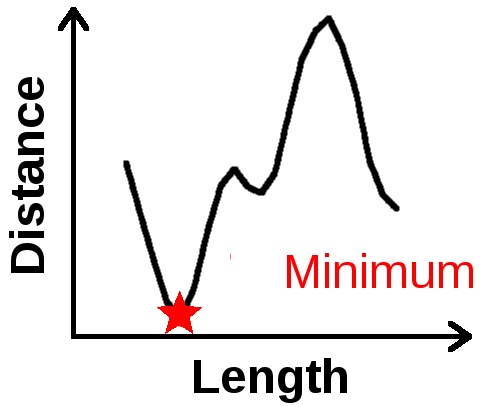
\includegraphics[width=1.25in]{distance_minimization.png} \\
				\par
			}
		\end{column}

	\end{columns}
	
	
	\begin{tikzpicture}[overlay, x=1cm,y=1cm]
		% Coordinates
		\coordinate (x1a) at (7, 5.25) ;
		\coordinate (x1b) at (3.5, 4) ;
		
		\coordinate (x2a) at (2, 4.75) ;
		\coordinate (x2b) at (1.75, 3.5) ;
		
		\coordinate (x3a) at (3, 1.35) ;
		\coordinate (x3b) at (4, 1.95) ;
		
		\coordinate (x4a) at (6.0, 1.95) ;
		\coordinate (x4b) at (8.05, 1.25) ;


		    		    
		% Arrow
		\path[draw=red,thick,->] (x1a) to[bend right] (x1b) ;
		
		\path[draw=red,thick,->] (x2a) to[bend right] (x2b) ;
		
		\path[draw=red,thick,->] (x3a) to[bend right] (x3b) ;

		\path[draw=red,thick,->] (x4a) to[bend right] (x4b) ;
		


		


			
	\end{tikzpicture}
	
	


\end{frame}





%%%%%%%%%%%%%%%%%%%%%%%%%%%%%%%%%%%%%%%%%%%%%%%%%%%%%%%%%%%%%%%%%%%%%%%%%%%%%%%%%%%%%%%%%%%%%%%%%%%%%%%%%%%%%%%%%%%%%%%%%%%%
% Length measurement experimental platform
%%%%%%%%%%%%%%%%%%%%%%%%%%%%%%%%%%%%%%%%%%%%%%%%%%%%%%%%%%%%%%%%%%%%%%%%%%%%%%%%%%%%%%%%%%%%%%%%%%%%%%%%%%%%%%%%%%%%%%%%%%%%

\begin{frame}[c]{Length measurement experimental test}
	\textcolor{negativered}{Can we implement and test the length measurement protocol?} \\
	\begin{itemize}
		\item Experiments were conducted with single pores etched into PET membranes $\left(D\sim\SI{750}{nm}, L=\SI{12}{\mu m}\right)$
		\item Three types of particles were tested
		\begin{itemize}
			\item $280$ and $\SI{410}{nm}$ polystyrene beads  (`spheres')
			\item $\SI{590}{nm}$ silica rods (`short rods')
			\item $\SI{1920}{nm}$ silica rods (`long rods')
		\end{itemize}
	\end{itemize}
	
	\begin{columns}[t]
		\begin{column}[T]{2.25in}
			{\centering
				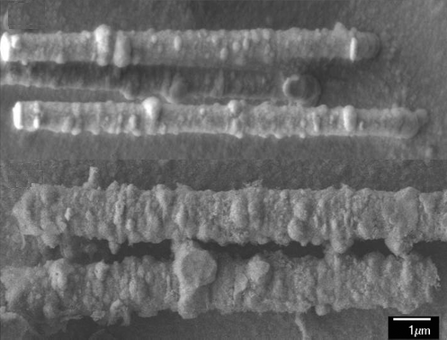
\includegraphics[height=0.75in]{PET.png} \\
				PET pore metal replica \\
				\par
			}
		\end{column}
		
		\begin{column}[T]{2.25in}
			{\centering
				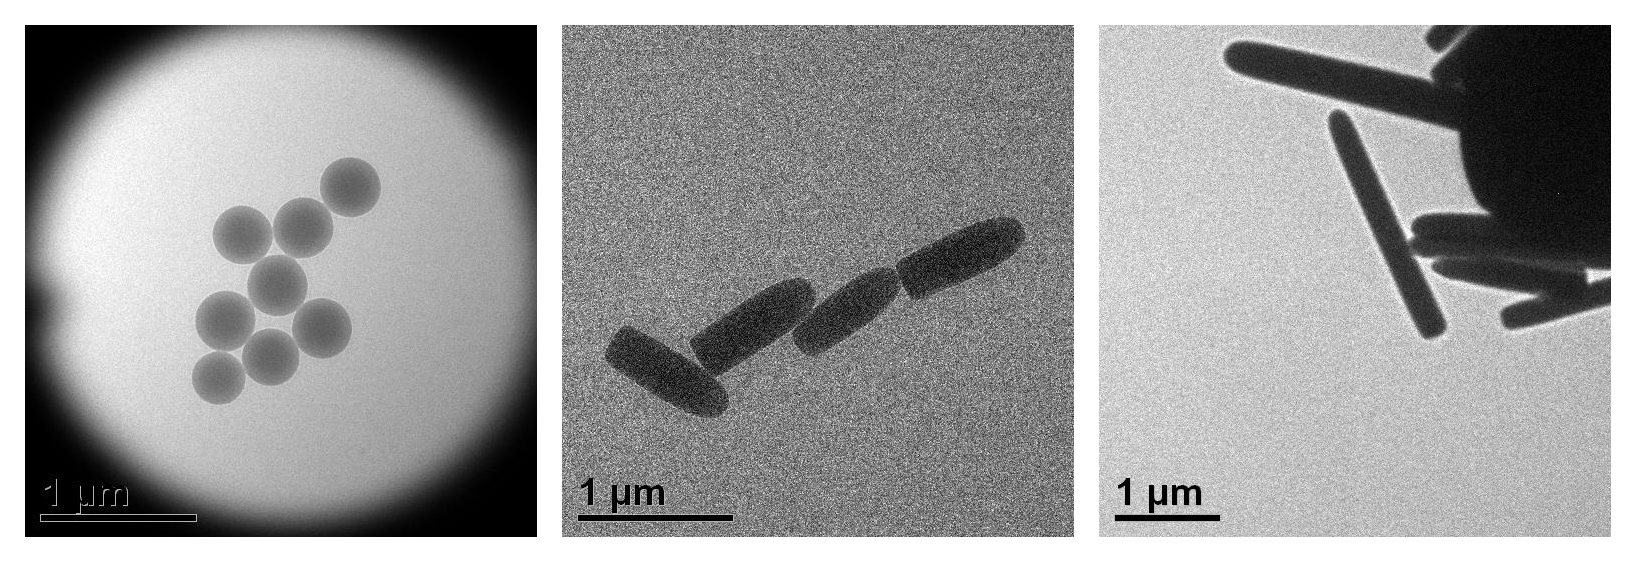
\includegraphics[height=0.75in]{particles.png} \\
				Nanoparticles \\
				\par				
			}
		\end{column}

	\end{columns}



\end{frame}


%%%%%%%%%%%%%%%%%%%%%%%%%%%%%%%%%%%%%%%%%%%%%%%%%%%%%%%%%%%%%%%%%%%%%%%%%%%%%%%%%%%%%%%%%%%%%%%%%%%%%%%%%%%%%%%%%%%%%%%%%%%%
% Length measurement experimental platform
%%%%%%%%%%%%%%%%%%%%%%%%%%%%%%%%%%%%%%%%%%%%%%%%%%%%%%%%%%%%%%%%%%%%%%%%%%%%%%%%%%%%%%%%%%%%%%%%%%%%%%%%%%%%%%%%%%%%%%%%%%%%

\begin{frame}[c]{Particles to scale}
	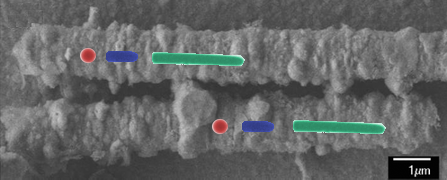
\includegraphics[width=4.5in]{particles_real_size.png}
\end{frame}



%%%%%%%%%%%%%%%%%%%%%%%%%%%%%%%%%%%%%%%%%%%%%%%%%%%%%%%%%%%%%%%%%%%%%%%%%%%%%%%%%%%%%%%%%%%%%%%%%%%%%%%%%%%%%%%%%%%%%%%%%%%%
% Resistive pulse background---system components
%%%%%%%%%%%%%%%%%%%%%%%%%%%%%%%%%%%%%%%%%%%%%%%%%%%%%%%%%%%%%%%%%%%%%%%%%%%%%%%%%%%%%%%%%%%%%%%%%%%%%%%%%%%%%%%%%%%%%%%%%%%%


\begin{frame}[c]{Polymer nanopore experiment components}



	\begin{columns}[t]
		\begin{column}[T]{\paperwidth/5}
			{\centering
				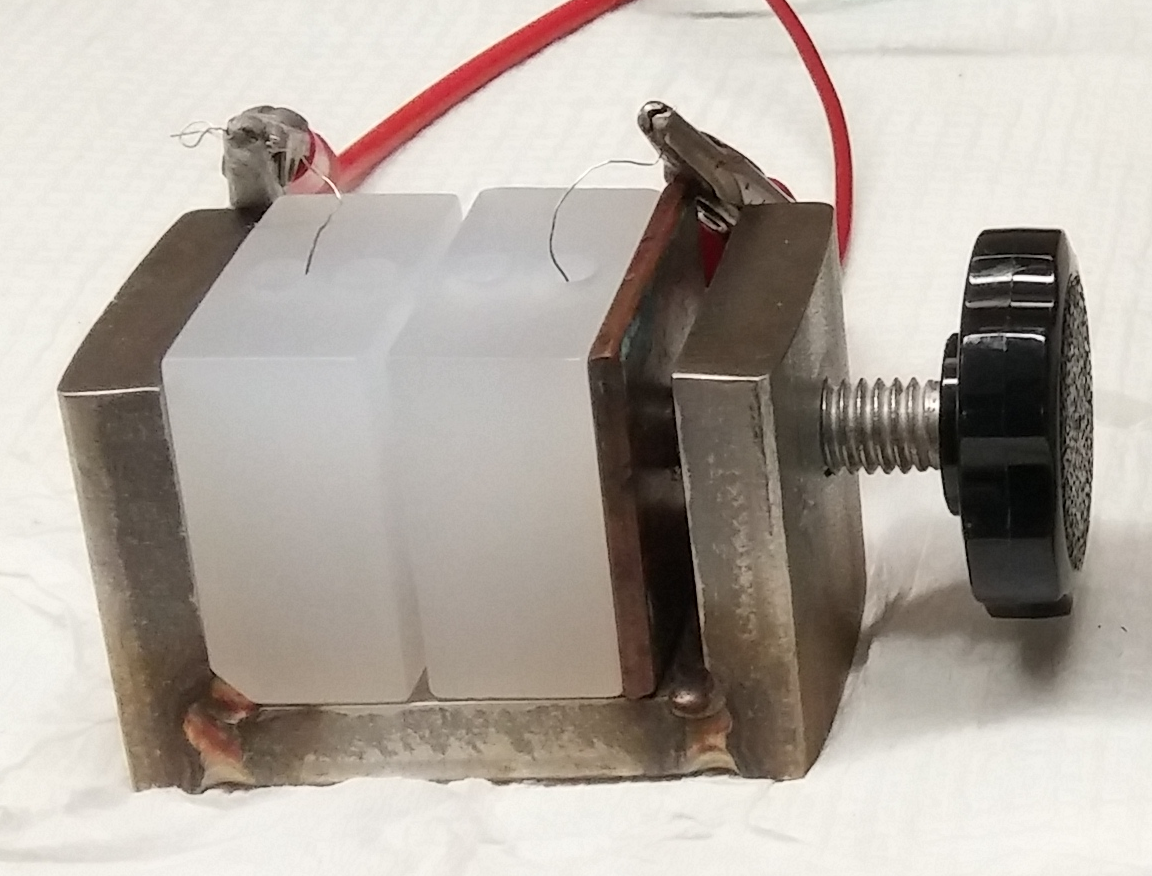
\includegraphics[height=2.25cm]{photo/conductivitycell.png} \\
				{\footnotesize Conductivity cell}
				\par
			}
		\end{column}
		
		
		\begin{column}[T]{\paperwidth/5}
			{\centering
				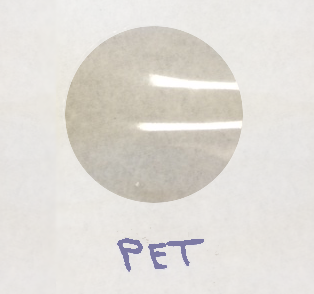
\includegraphics[height=2.25cm]{photo/PETmembrane.png} \\
				{\footnotesize Pore membrane}
				\par
			}
		\end{column}
		
		
		
		\begin{column}[T]{\paperwidth/5}
			{\centering
				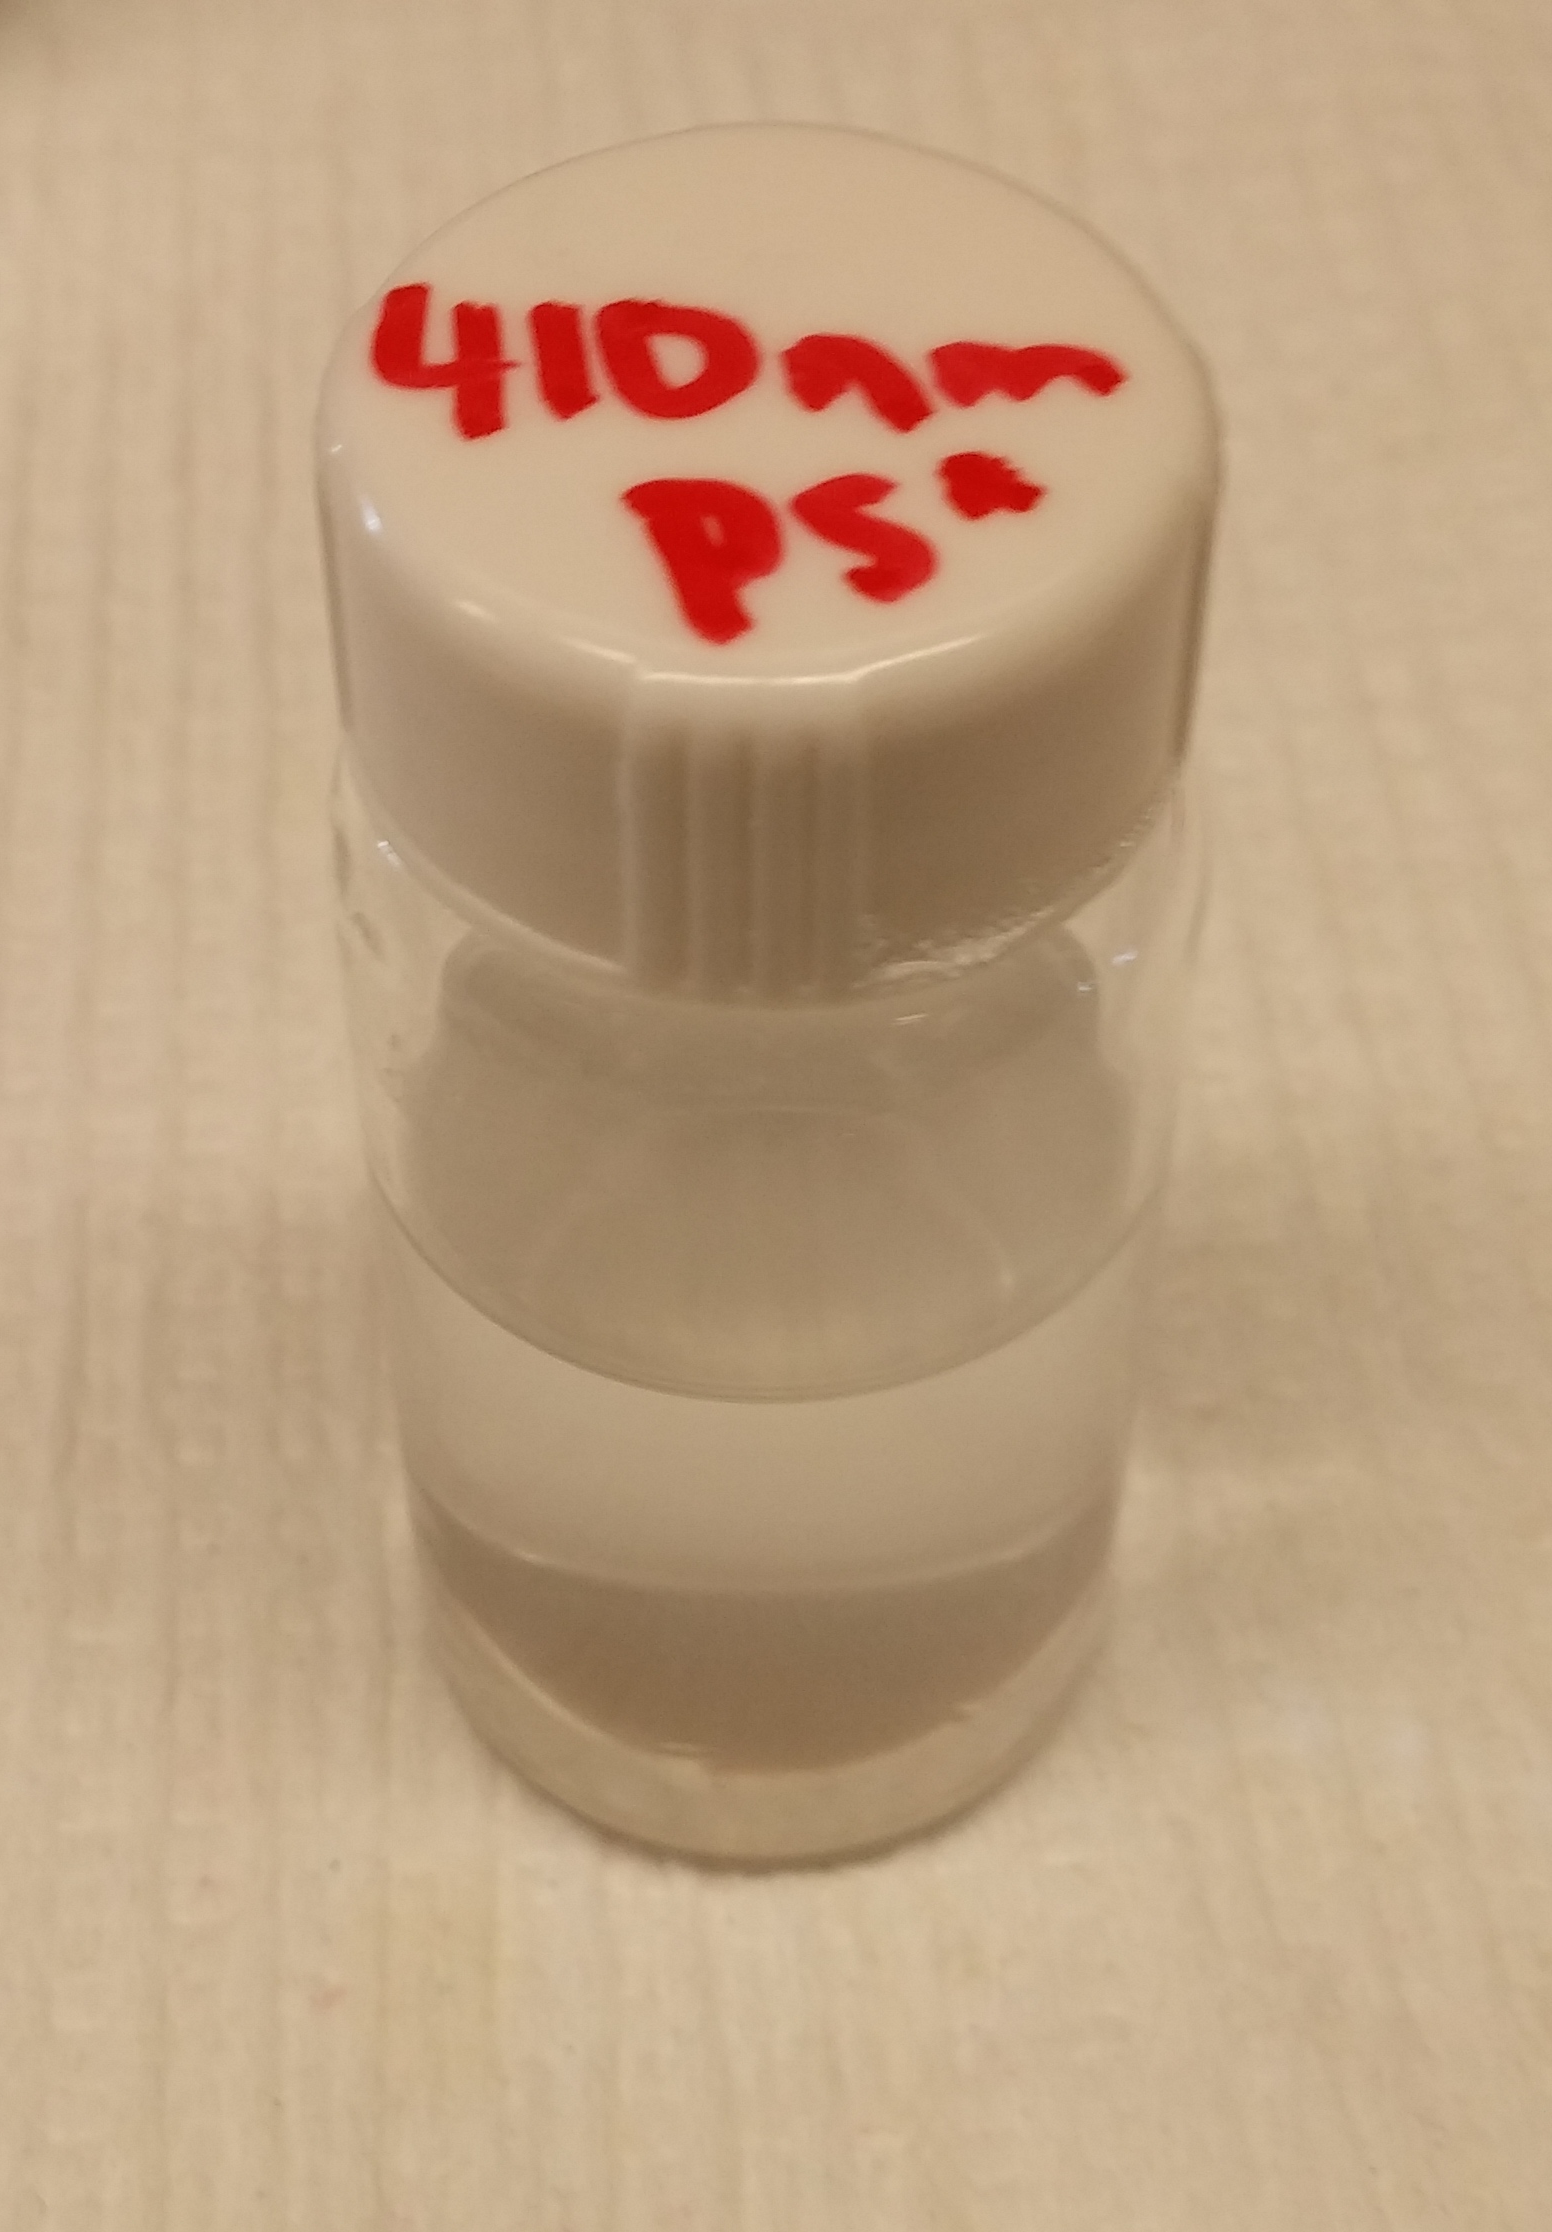
\includegraphics[height=2.25cm]{photo/solution.png} \\
				{\footnotesize Electrolyte}
				\par
			}
		\end{column}

		
		

		
		\begin{column}[T]{\paperwidth/5}
			{\centering
				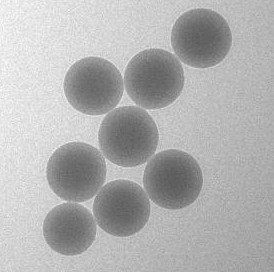
\includegraphics[height=2.25cm]{psbeads} \\
				{\footnotesize Particles}
				\par
			}
		\end{column}

	\end{columns}
	
	\vspace{1cm}
	
	\begin{columns}[t]
		\begin{column}[T]{\paperwidth/5}
			{\centering
				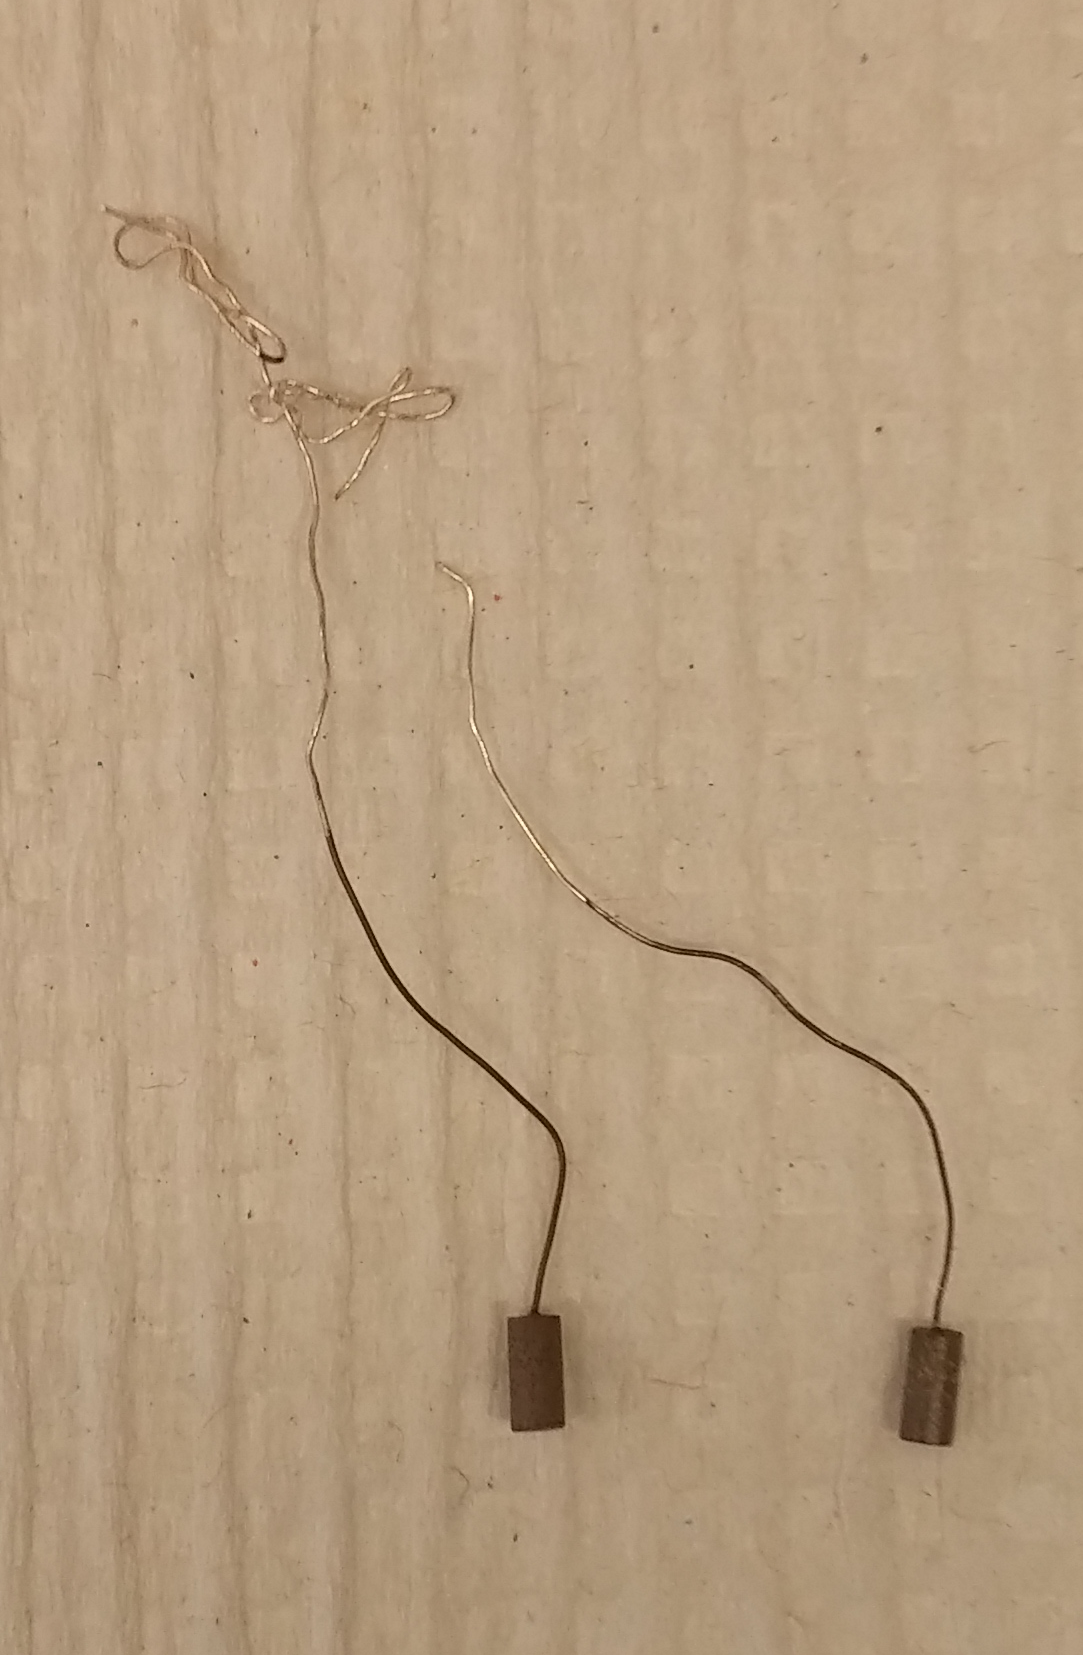
\includegraphics[height=2.25cm]{photo/electrodes.png} \\
				{\footnotesize Ag-AgCl electrodes}
				\par
			}
		\end{column}
		
		
		\begin{column}[T]{.6\paperwidth}
			{\centering
				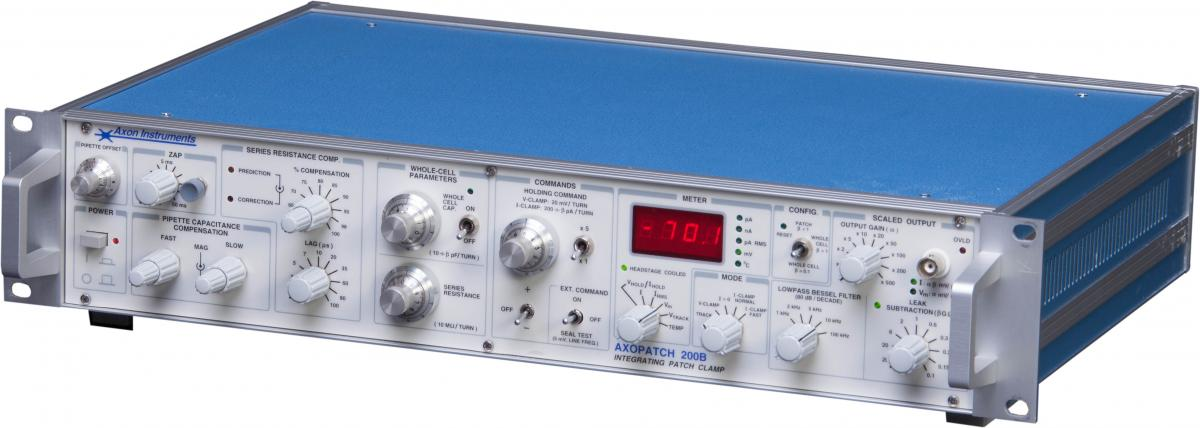
\includegraphics[height=2.25cm]{photo/axon200b} \\
				Voltage amplifier + current recorder
				\par
			}
		\end{column}
	

	\end{columns}


\end{frame}



%%%%%%%%%%%%%%%%%%%%%%%%%%%%%%%%%%%%%%%%%%%%%%%%%%%%%%%%%%%%%%%%%%%%%%%%%%%%%%%%%%%%%%%%%%%%%%%%%%%%%%%%%%%%%%%%%%%%%%%%%%%%
% Results---raw data
%%%%%%%%%%%%%%%%%%%%%%%%%%%%%%%%%%%%%%%%%%%%%%%%%%%%%%%%%%%%%%%%%%%%%%%%%%%%%%%%%%%%%%%%%%%%%%%%%%%%%%%%%%%%%%%%%%%%%%%%%%%%

\begin{frame}[c]{Results---raw data}

	{\centering
		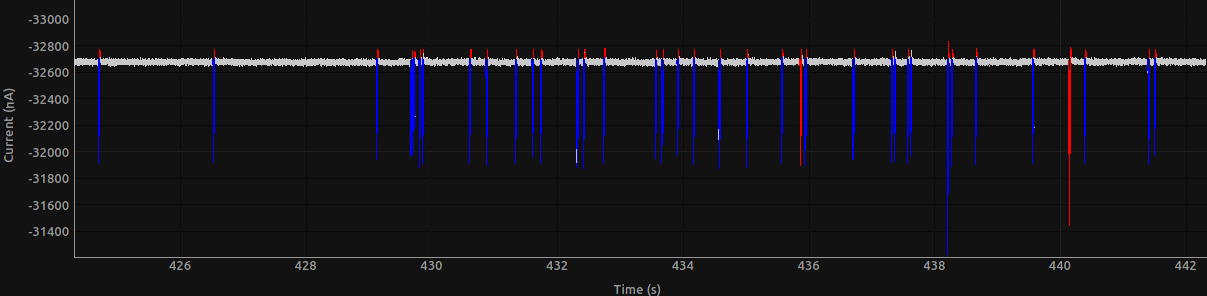
\includegraphics[width=3.75in]{experiment_timeseries.png} \\
		Resistive pulse time series \\
		\par
	}
	
	\begin{columns}[t]
		\begin{column}[T]{2.25in}
			{\centering
				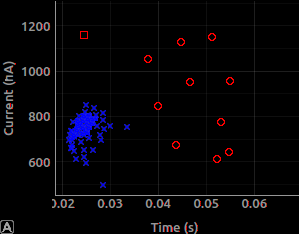
\includegraphics[height=1.25in]{experiment_scatter.png} \\
				Amplitude-duration scatter
				\par
			}
		\end{column}
		
		\begin{column}[T]{2.25in}
			{\centering
				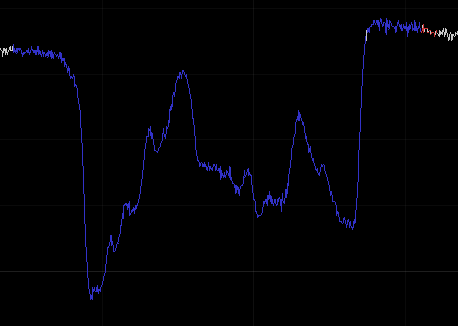
\includegraphics[height=1.25in]{experiment_singleevent.png} \\
				Raw event \\
				\par
			}
		\end{column}

	\end{columns}
	
\end{frame}






%%%%%%%%%%%%%%%%%%%%%%%%%%%%%%%%%%%%%%%%%%%%%%%%%%%%%%%%%%%%%%%%%%%%%%%%%%%%%%%%%%%%%%%%%%%%%%%%%%%%%%%%%%%%%%%%%%%%%%%%%%%%
% Results---PET21---Raw
%%%%%%%%%%%%%%%%%%%%%%%%%%%%%%%%%%%%%%%%%%%%%%%%%%%%%%%%%%%%%%%%%%%%%%%%%%%%%%%%%%%%%%%%%%%%%%%%%%%%%%%%%%%%%%%%%%%%%%%%%%%%
 
 \begin{frame}[c]{Results---sphere, short rod, and long rod events}
 	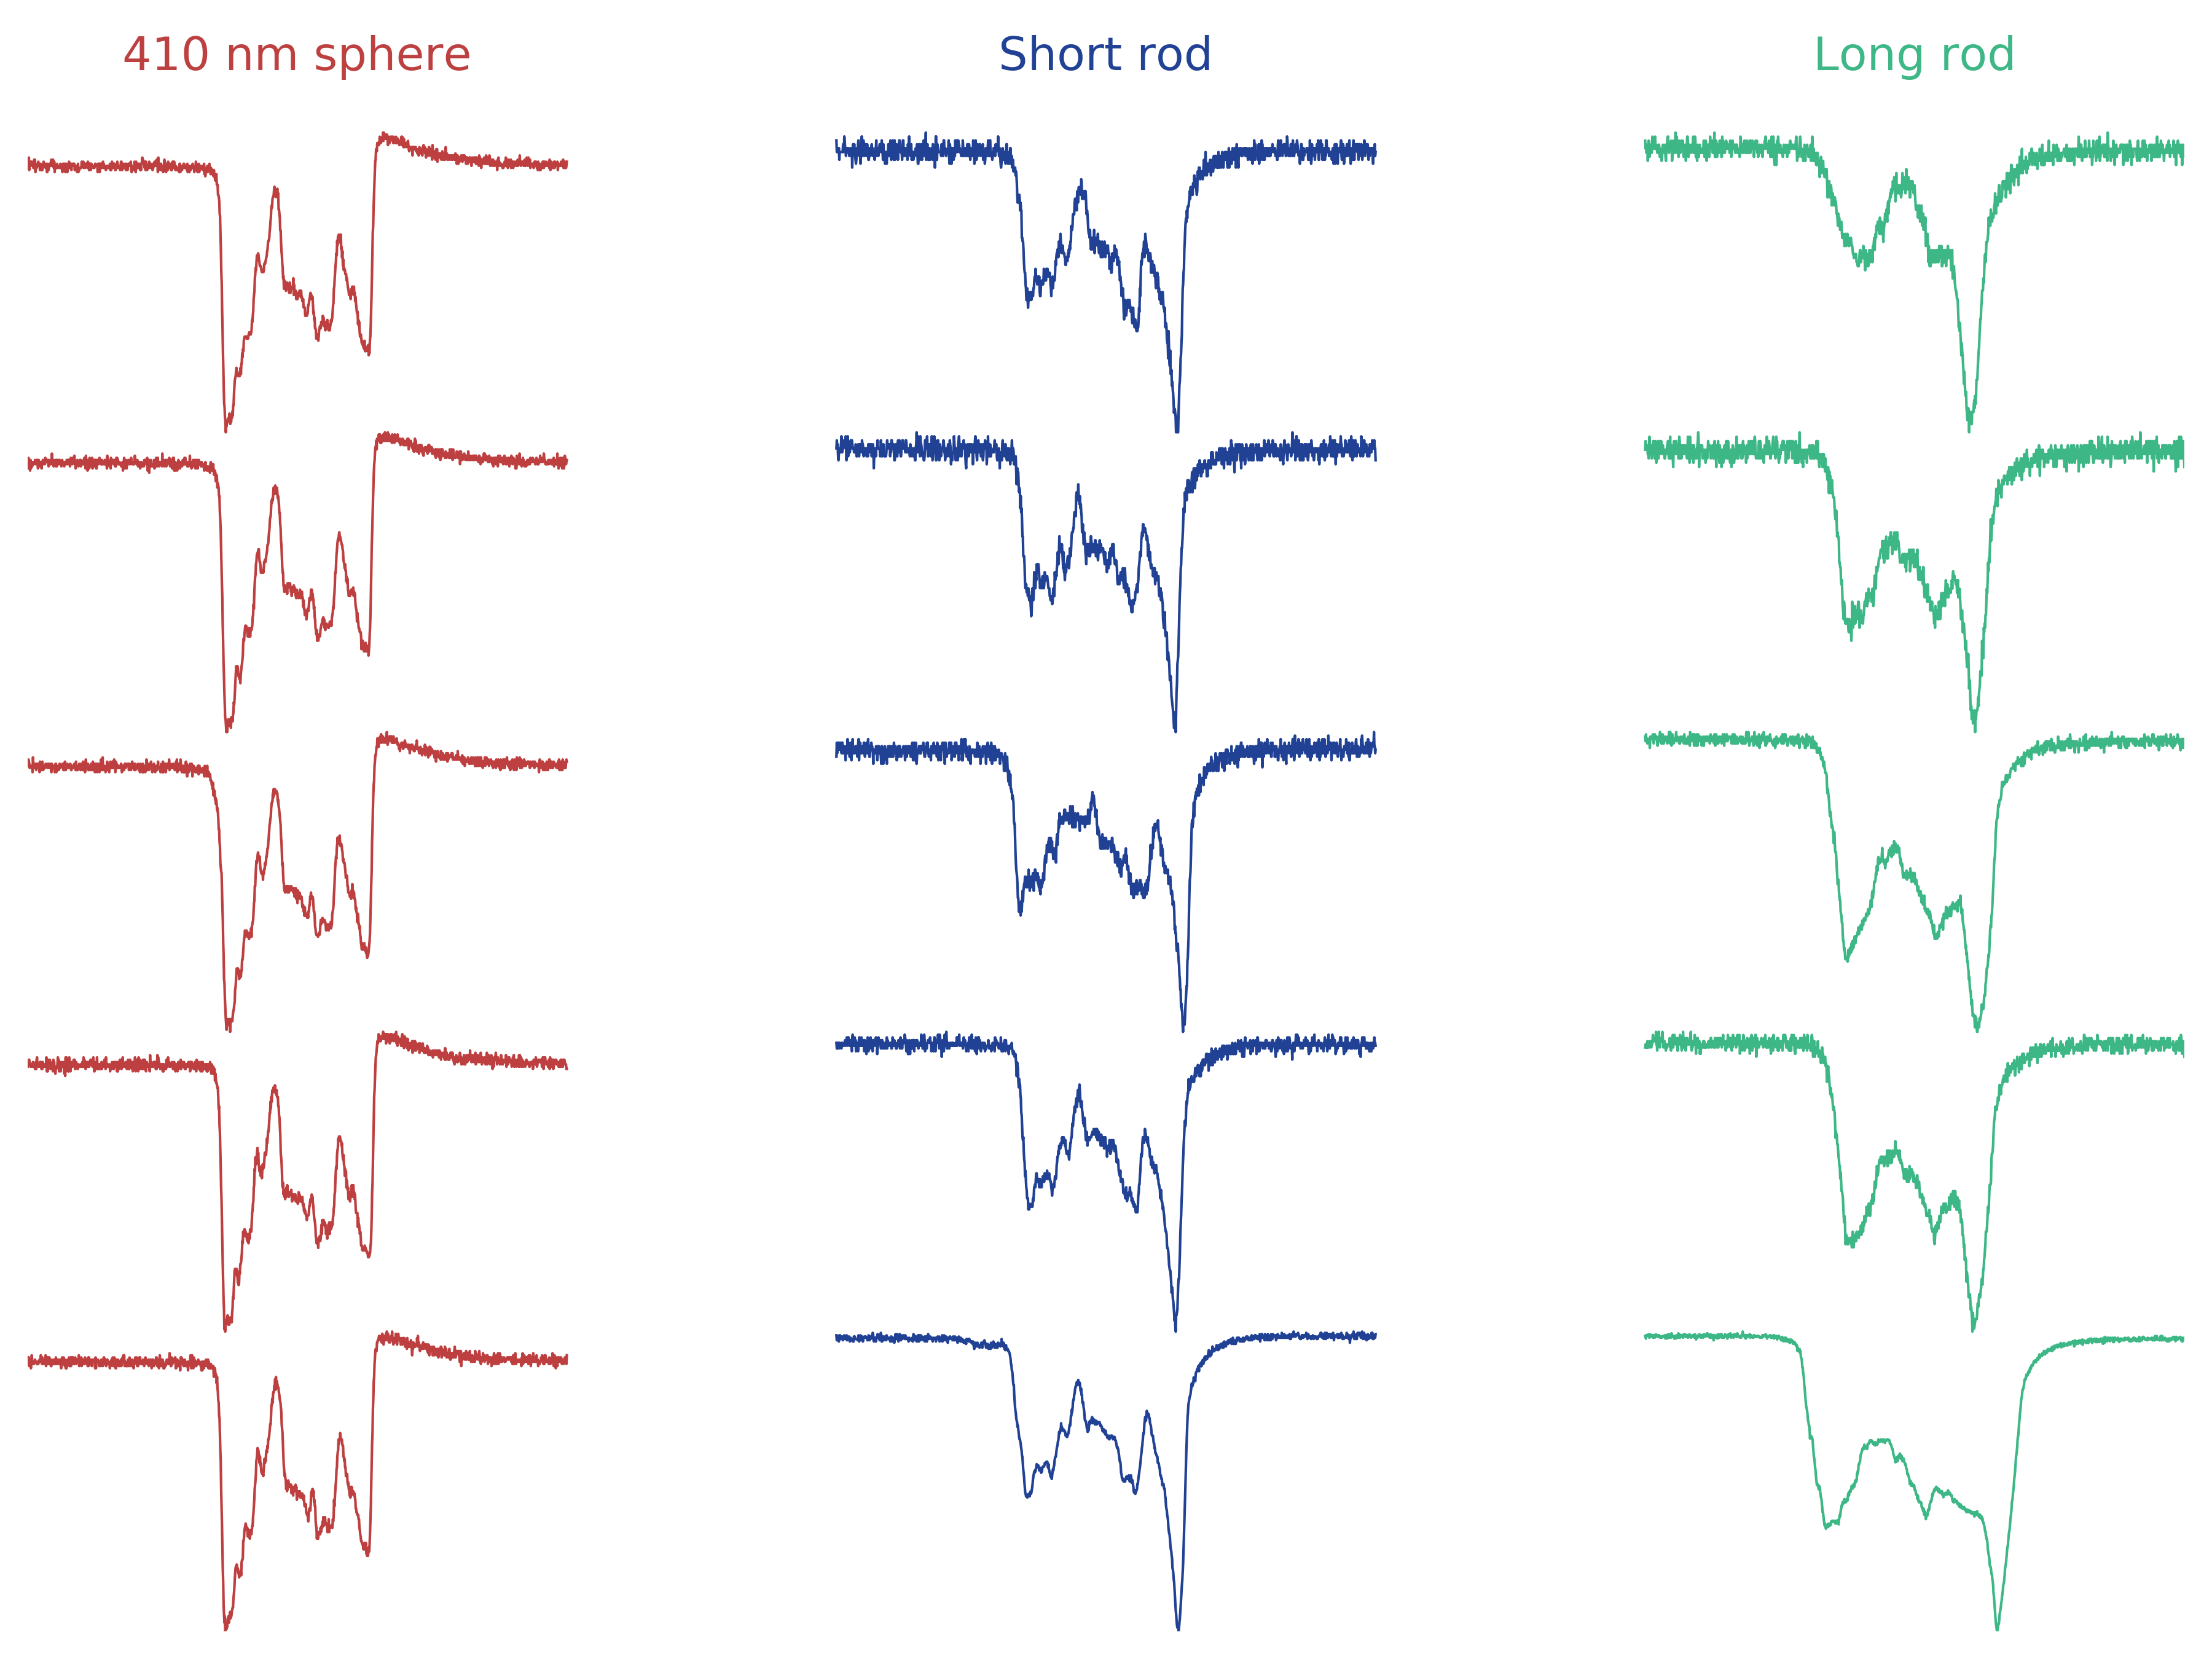
\includegraphics[width=4.25in]{PET21_raw.png}
 \end{frame}

 
% %%%%%%%%%%%%%%%%%%%%%%%%%%%%%%%%%%%%%%%%%%%%%%%%%%%%%%%%%%%%%%%%%%%%%%%%%%%%%%%%%%%%%%%%%%%%%%%%%%%%%%%%%%%%%%%%%%%%%%%%%%%%
% % Results---PET21---Smoothed
% %%%%%%%%%%%%%%%%%%%%%%%%%%%%%%%%%%%%%%%%%%%%%%%%%%%%%%%%%%%%%%%%%%%%%%%%%%%%%%%%%%%%%%%%%%%%%%%%%%%%%%%%%%%%%%%%%%%%%%%%%%%%
% 
% \begin{frame}[c]{Results---PET21 averaged events}
% 	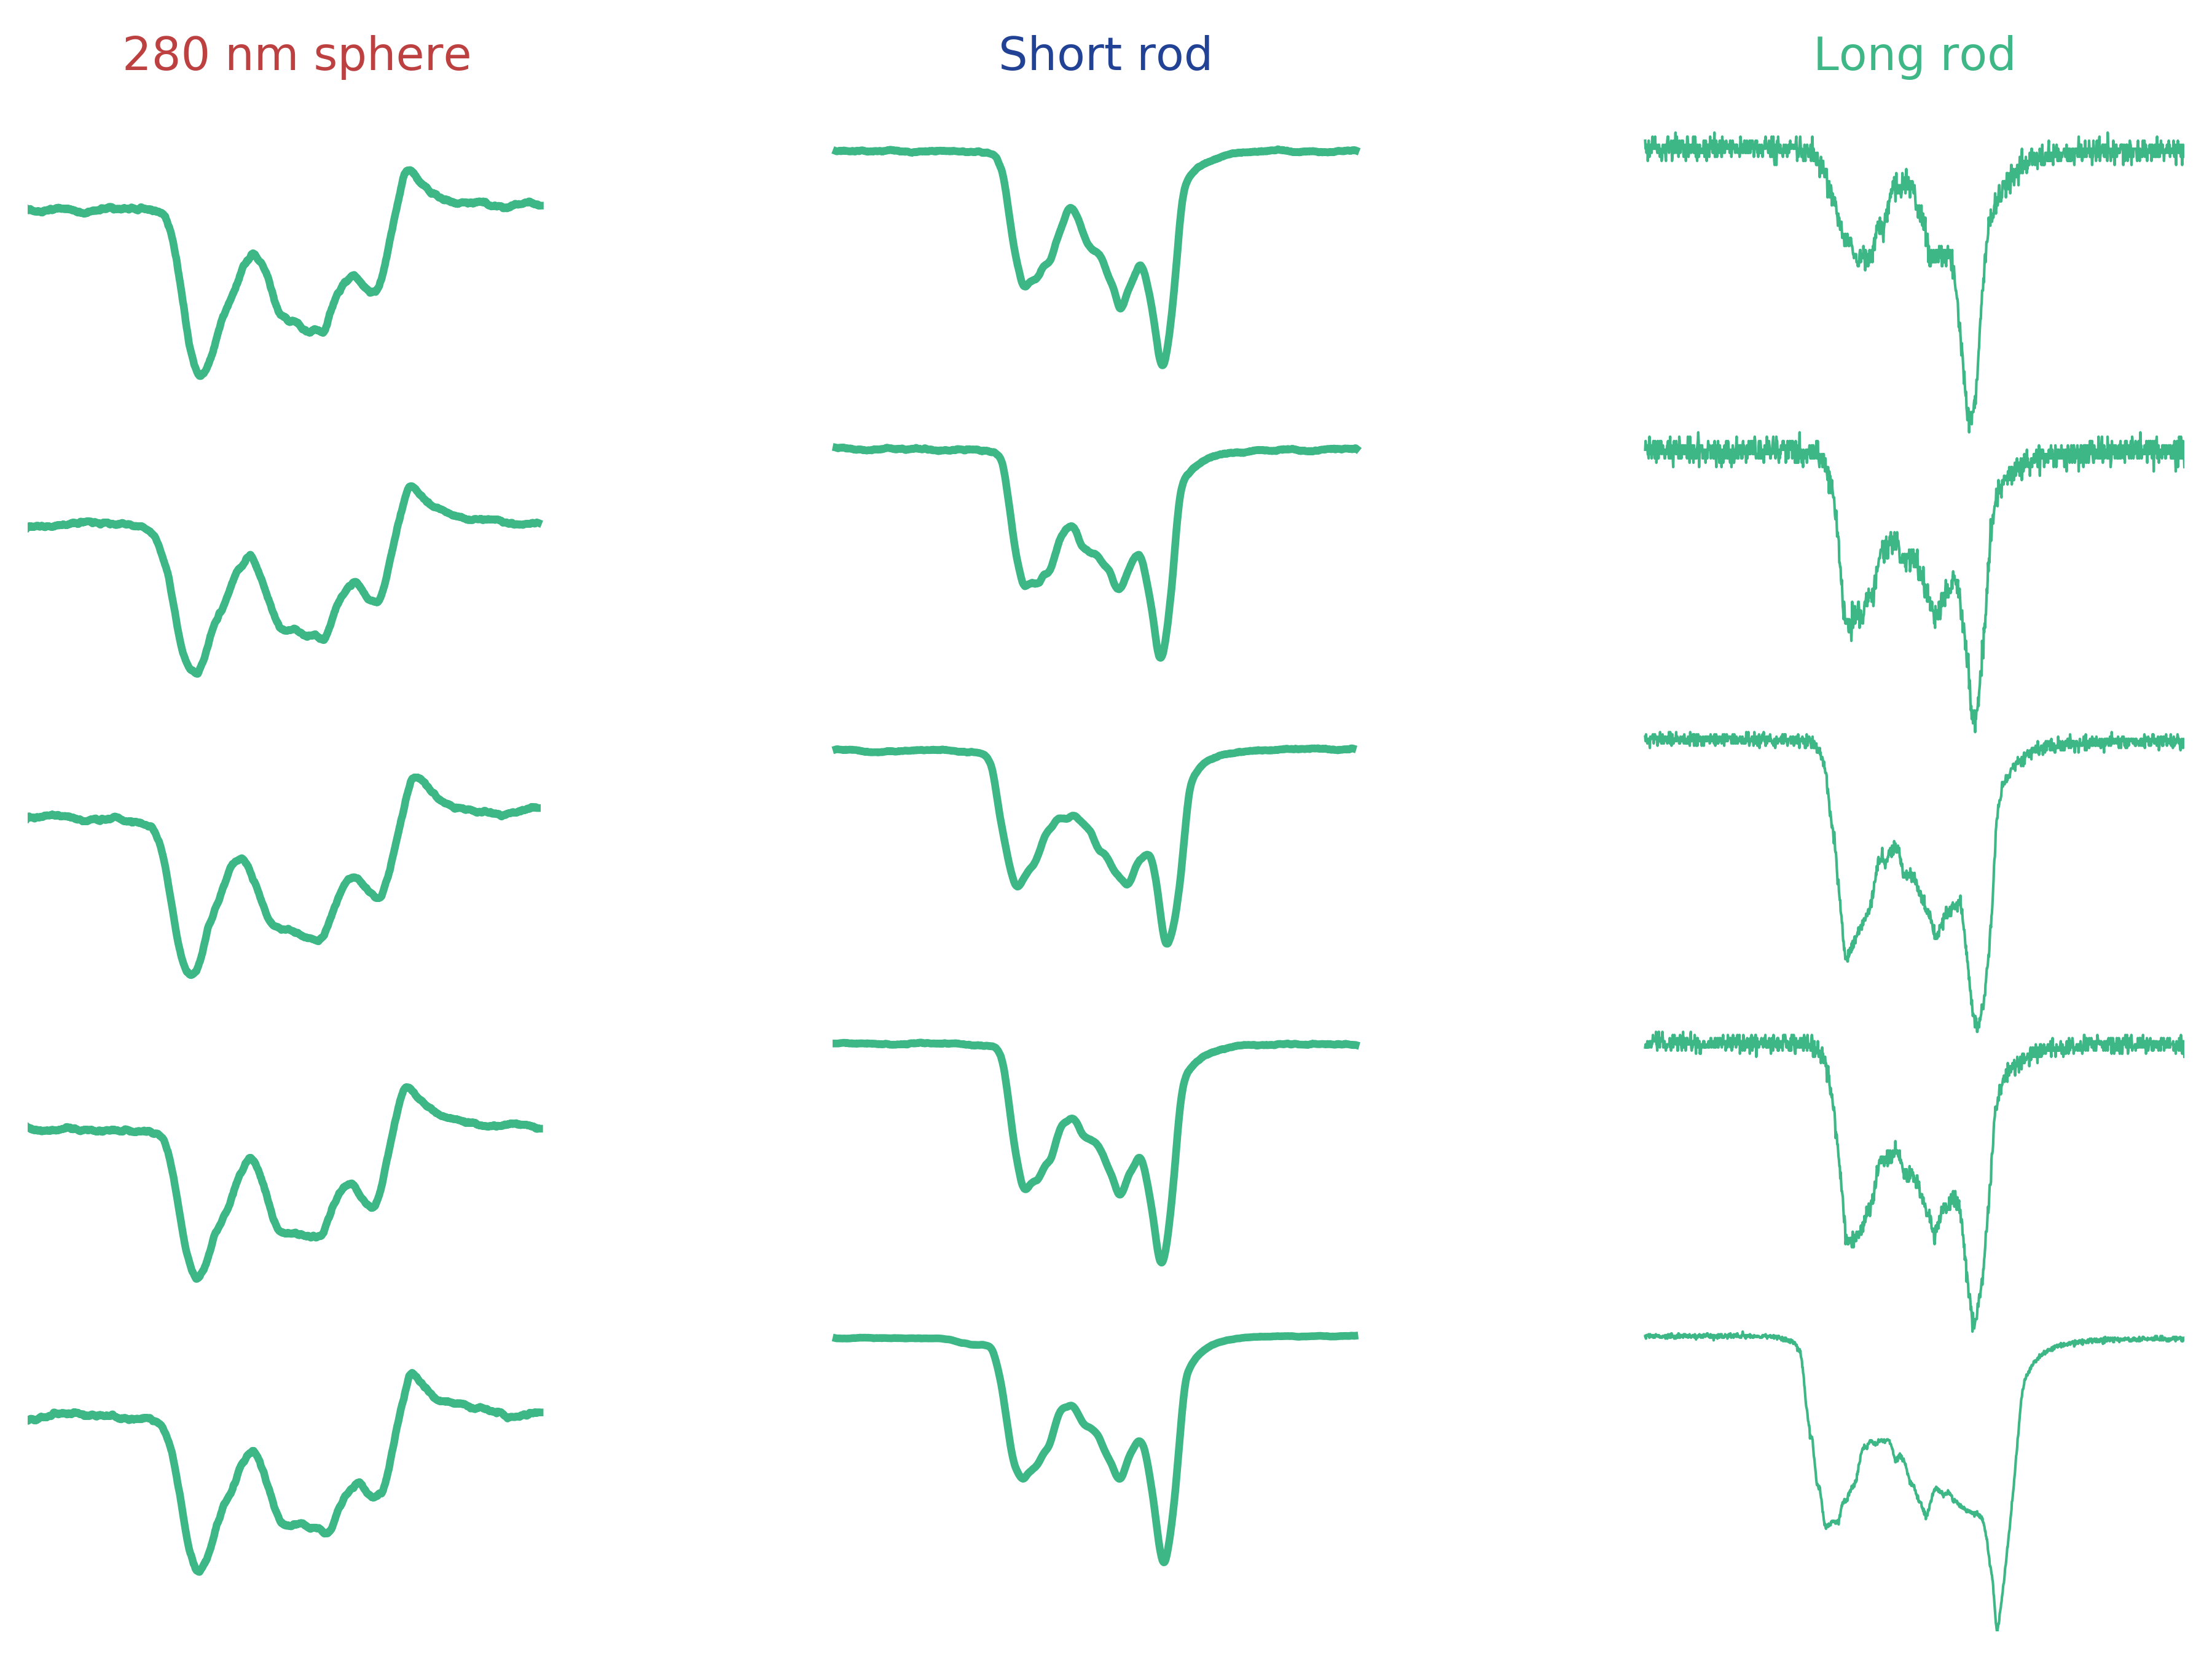
\includegraphics[width=4.5in]{PET21_averaged.png}
% \end{frame}




%%%%%%%%%%%%%%%%%%%%%%%%%%%%%%%%%%%%%%%%%%%%%%%%%%%%%%%%%%%%%%%%%%%%%%%%%%%%%%%%%%%%%%%%%%%%%%%%%%%%%%%%%%%%%%%%%%%%%%%%%%%%
% Results---PET7---Raw and averaged event comparison
%%%%%%%%%%%%%%%%%%%%%%%%%%%%%%%%%%%%%%%%%%%%%%%%%%%%%%%%%%%%%%%%%%%%%%%%%%%%%%%%%%%%%%%%%%%%%%%%%%%%%%%%%%%%%%%%%%%%%%%%%%%%

\begin{frame}[c]{Results---Qualitative event comparison}
	% Add citation
	
	{\centering
		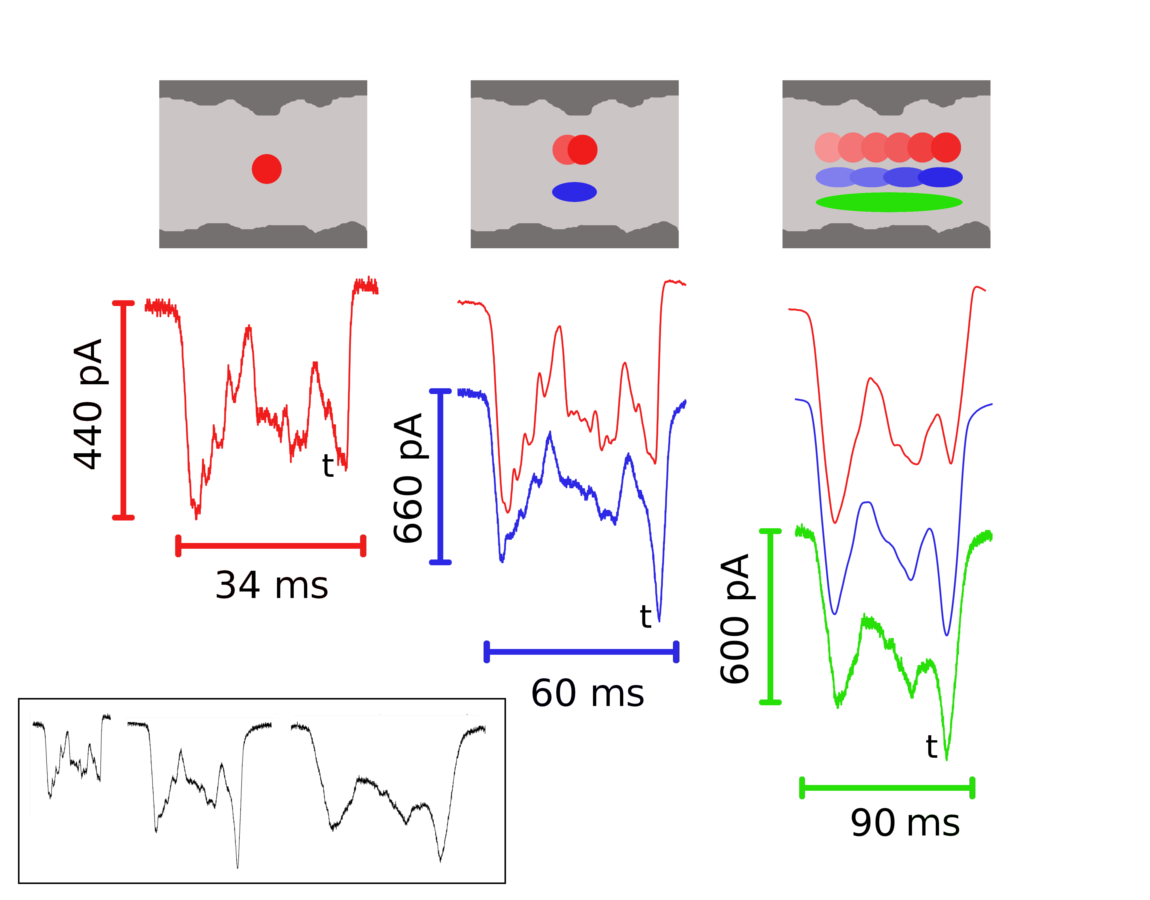
\includegraphics[width=2.5in]{PETevents.png} \\
		{\tiny Qiu \textit{et al.} \textit{ACS Nano} \textbf{9}, 4390-4397 (2015).} \\
		\vspace{.2in}
		\textcolor{negativered}{The averaging process produces signals that are qualitatively similar to the observed signals of longer particles}
		\par
	}
\end{frame}



%%%%%%%%%%%%%%%%%%%%%%%%%%%%%%%%%%%%%%%%%%%%%%%%%%%%%%%%%%%%%%%%%%%%%%%%%%%%%%%%%%%%%%%%%%%%%%%%%%%%%%%%%%%%%%%%%%%%%%%%%%%%
% Results---PET7---Raw and smoothed
%%%%%%%%%%%%%%%%%%%%%%%%%%%%%%%%%%%%%%%%%%%%%%%%%%%%%%%%%%%%%%%%%%%%%%%%%%%%%%%%%%%%%%%%%%%%%%%%%%%%%%%%%%%%%%%%%%%%%%%%%%%%

\begin{frame}[c]{Results---Quantitative event comparison}
	{\centering
		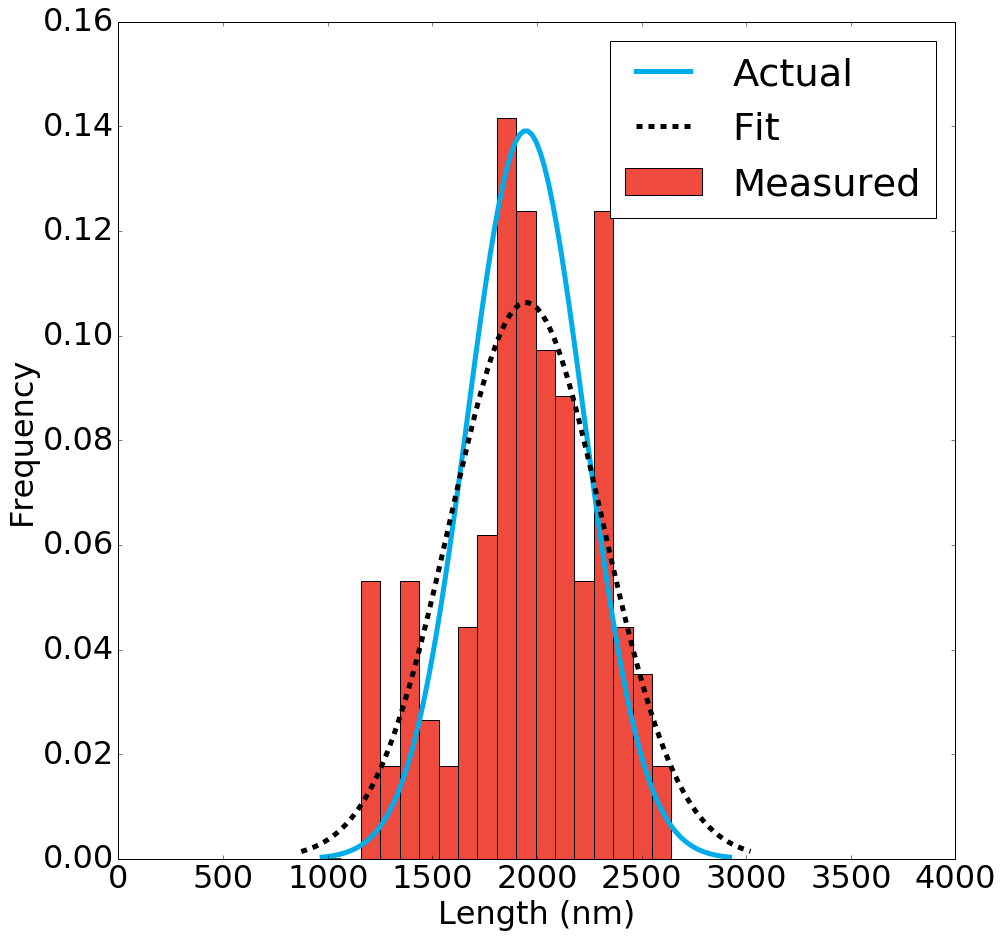
\includegraphics[width=2.75in]{dtwfit.png} \\
		\textcolor{negativered}{Quantitative measurement of particle length yields a distribution closely matching the actual distribution of lengths!}
		\par
	}
\end{frame}



%%%%%%%%%%%%%%%%%%%%%%%%%%%%%%%%%%%%%%%%%%%%%%%%%%%%%%%%%%%%%%%%%%%%%%%%%%%%%%%%%%%%%%%%%%%%%%%%%%%%%%%%%%%%%%%%%%%%%%%%%%%%
% Future work
%%%%%%%%%%%%%%%%%%%%%%%%%%%%%%%%%%%%%%%%%%%%%%%%%%%%%%%%%%%%%%%%%%%%%%%%%%%%%%%%%%%%%%%%%%%%%%%%%%%%%%%%%%%%%%%%%%%%%%%%%%%%

\begin{frame}[c]{Conclusions \& Future work}

	\only<1>{
		{\centering
			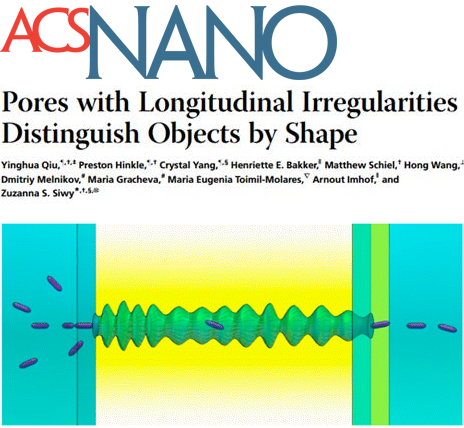
\includegraphics[width=2.75in]{paper/acsnano.png} \\ 
			\par
		}
	}
      
	% Too wordy

	\only<2>{
		It's apparent that the model for how particles map the interiors of pores is accurate \\
		\vspace{.2in}
		Some things left for the future: \\
		\begin{enumerate}
			\item Test robustness of quantitative length measurement
			\item Run length measurement protocol on particles of various unknown lengths, test results
			\item Reduce system scale: Test length measurement protocol with fabricated nanochannels with controlled geometries
		\end{enumerate}
	}
\end{frame}



%%%%%%%%%%%%%%%%%%%%%%%%%%%%%%%%%%%%%%%%%%%%%%%%%%%%%%%%%%%%%%%%%%%%%%%%%%%%%%%%%%%%%%%%%%%%%%%%%%%%%%%%%%%%%%%%%%%%%%%%%%%%
% RP-IM title slide
%%%%%%%%%%%%%%%%%%%%%%%%%%%%%%%%%%%%%%%%%%%%%%%%%%%%%%%%%%%%%%%%%%%%%%%%%%%%%%%%%%%%%%%%%%%%%%%%%%%%%%%%%%%%%%%%%%%%%%%%%%%%


\begin{frame}[c]{}
	\begin{center}
		\textbf{Hybrid imaging-resistive pulse measurements in microfluidic channels}
	\end{center}
\end{frame}



%%%%%%%%%%%%%%%%%%%%%%%%%%%%%%%%%%%%%%%%%%%%%%%%%%%%%%%%%%%%%%%%%%%%%%%%%%%%%%%%%%%%%%%%%%%%%%%%%%%%%%%%%%%%%%%%%%%%%%%%%%%%
% RP-IM motivation 1
%%%%%%%%%%%%%%%%%%%%%%%%%%%%%%%%%%%%%%%%%%%%%%%%%%%%%%%%%%%%%%%%%%%%%%%%%%%%%%%%%%%%%%%%%%%%%%%%%%%%%%%%%%%%%%%%%%%%%%%%%%%%


\begin{frame}[c]{Motivation---Why introduce optics?}
	
	In an RP experiment, the usual parameters measured are amplitude and duration, which can relate to particle's volume, charge, etc. \\
	\vspace{.3in}
	But, the equations which relate the RP signal to physical observables are only accurate under sterile conditions \\
	\vspace{.3in}
 	In reality, the experimental setup can seldom be constrained to this degree \\
 	

\end{frame}



%%%%%%%%%%%%%%%%%%%%%%%%%%%%%%%%%%%%%%%%%%%%%%%%%%%%%%%%%%%%%%%%%%%%%%%%%%%%%%%%%%%%%%%%%%%%%%%%%%%%%%%%%%%%%%%%%%%%%%%%%%%%
% RP-IM motivation 2
%%%%%%%%%%%%%%%%%%%%%%%%%%%%%%%%%%%%%%%%%%%%%%%%%%%%%%%%%%%%%%%%%%%%%%%%%%%%%%%%%%%%%%%%%%%%%%%%%%%%%%%%%%%%%%%%%%%%%%%%%%%%


\begin{frame}[c]{Motivation---Why introduce optics?}
	

	
	Some confounding factors include
	
	\begin{itemize}
		\item Entrance effects in low or medium aspect ratio pores
		\item Non-spheroidal particles, rotational effects
		\item Off-axis translocation
	\end{itemize}
	
	The influence of each of these effects on the RP signal is difficult to measure

\end{frame}



%%%%%%%%%%%%%%%%%%%%%%%%%%%%%%%%%%%%%%%%%%%%%%%%%%%%%%%%%%%%%%%%%%%%%%%%%%%%%%%%%%%%%%%%%%%%%%%%%%%%%%%%%%%%%%%%%%%%%%%%%%%%
% RP-IM motivation 3
%%%%%%%%%%%%%%%%%%%%%%%%%%%%%%%%%%%%%%%%%%%%%%%%%%%%%%%%%%%%%%%%%%%%%%%%%%%%%%%%%%%%%%%%%%%%%%%%%%%%%%%%%%%%%%%%%%%%%%%%%%%%


\begin{frame}[c]{Motivation---Why introduce optics?}
	
	What if we could \textit{see} what is happening during a resistive pulse experiment? 
	
	\vspace{.2in}
	
	Then we could determine the influence of these confounding factors during the event translocation \\
	
	\vspace{.2in}
	
	For instance, we could directly observe the effect of off-axis translocation on the resistive pulse signal
	
	\vspace{.2in}
	
	The results would generalize to other resistive pulse experiments and lead to greater interpretability of the RP signals!  \\
	

\end{frame}


%%%%%%%%%%%%%%%%%%%%%%%%%%%%%%%%%%%%%%%%%%%%%%%%%%%%%%%%%%%%%%%%%%%%%%%%%%%%%%%%%%%%%%%%%%%%%%%%%%%%%%%%%%%%%%%%%%%%%%%%%%%%
% RP-IM motivation 4
%%%%%%%%%%%%%%%%%%%%%%%%%%%%%%%%%%%%%%%%%%%%%%%%%%%%%%%%%%%%%%%%%%%%%%%%%%%%%%%%%%%%%%%%%%%%%%%%%%%%%%%%%%%%%%%%%%%%%%%%%%%%


\begin{frame}[c]{Motivation---Why introduce optics?}
	
	But, the trouble is that directly imaging nanoscale resistive pulse experiments is extremely difficult; need an electron microscope that can operate \textit{in situ}
	
	\vspace{.2in}
	
	However, at the microscale we can use plain optics to image the experiments while simultaneously measuring the resistive pulses
	
	\vspace{.2in}
	
	The results should generalize to the nanoscale as well, since the confounding factors arise due to electrostatic boundary conditions that are scale independent
	
	\vspace{.2in}
	

\end{frame}


%%%%%%%%%%%%%%%%%%%%%%%%%%%%%%%%%%%%%%%%%%%%%%%%%%%%%%%%%%%%%%%%%%%%%%%%%%%%%%%%%%%%%%%%%%%%%%%%%%%%%%%%%%%%%%%%%%%%%%%%%%%%
% Experimental objective
%%%%%%%%%%%%%%%%%%%%%%%%%%%%%%%%%%%%%%%%%%%%%%%%%%%%%%%%%%%%%%%%%%%%%%%%%%%%%%%%%%%%%%%%%%%%%%%%%%%%%%%%%%%%%%%%%%%%%%%%%%%%


\begin{frame}[c]{Experimental objective}

	\textcolor{negativered}{Objective: Create a hybrid resistive pulse-optical characterization platform} \\
	
	\vspace{.1in}
	
	Essentially, we want to devise a micro-sized resistive pulse system that we can also image \\
	
	\vspace{.1in}
	
	This requires adding a few elements to the standard resistive pulse set up
	
	\begin{itemize}
		\item Optically transparent, planar microchannels
		\item Pressure-induced flow, e.g. via a syringe pump (electrophoresis and electroosmosis are less pronounced at this scale)
		\item Microscope to magnify the image
		\item High-speed camera to capture images
	\end{itemize}

	
	

\end{frame}


%%%%%%%%%%%%%%%%%%%%%%%%%%%%%%%%%%%%%%%%%%%%%%%%%%%%%%%%%%%%%%%%%%%%%%%%%%%%%%%%%%%%%%%%%%%%%%%%%%%%%%%%%%%%%%%%%%%%%%%%%%%%
% Device fabrication
%%%%%%%%%%%%%%%%%%%%%%%%%%%%%%%%%%%%%%%%%%%%%%%%%%%%%%%%%%%%%%%%%%%%%%%%%%%%%%%%%%%%%%%%%%%%%%%%%%%%%%%%%%%%%%%%%%%%%%%%%%%%


\begin{frame}[c]{PDMS channel fabrication}

	The channels were fabricated with PDMS, an optically transparent elastomer ideal for microfluidic experiments \\
	
	

	{\footnotesize
	\begin{enumerate}
		\item Channel design is printed onto a high-resolution phototransparency
		\item Channel design is then transferred to a mold via standard soft photolithography
		\item PDMS is poured over mold and removed after curing
		\item PDMS bonded to a glass slide using an oxygen plasma
	\end{enumerate}
	}
	
	
	\begin{columns}[t]
		\begin{column}[T]{1.67in}
			{\centering
				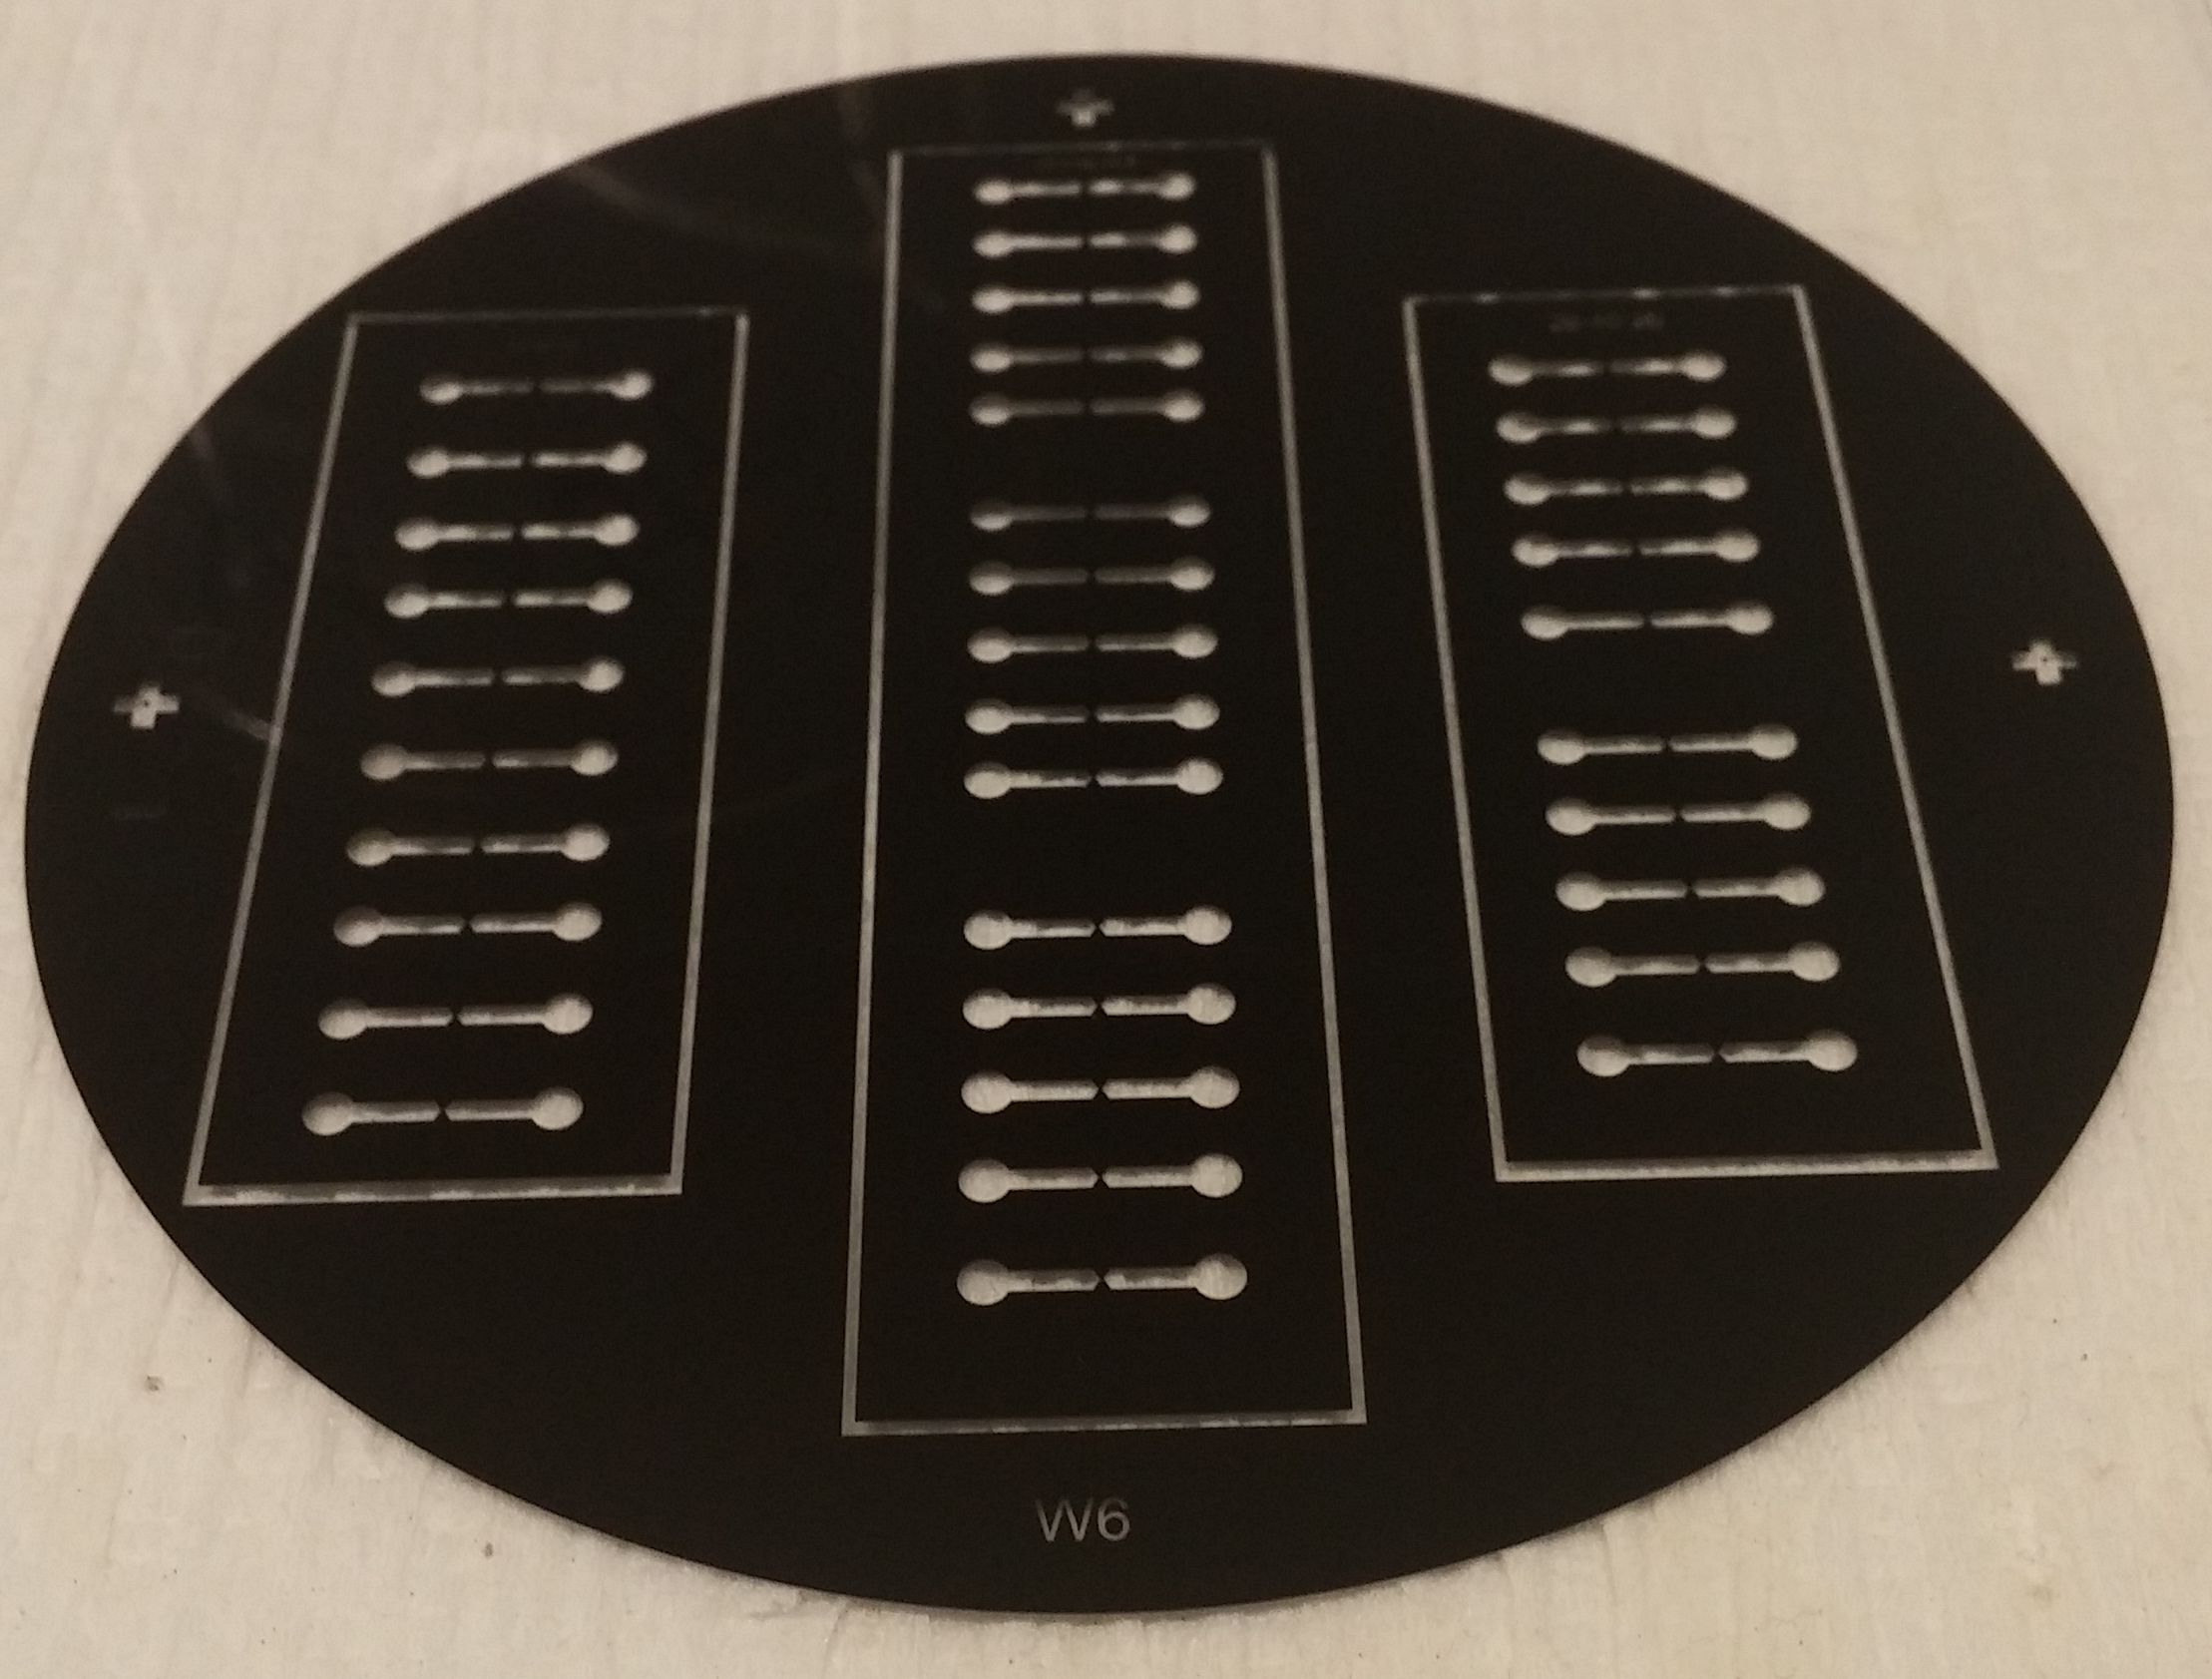
\includegraphics[height=.85in]{transparency} \\
				Phototransparency \\
				\par
			}
		\end{column}
		
		\begin{column}[T]{1.67in}
			{\centering
				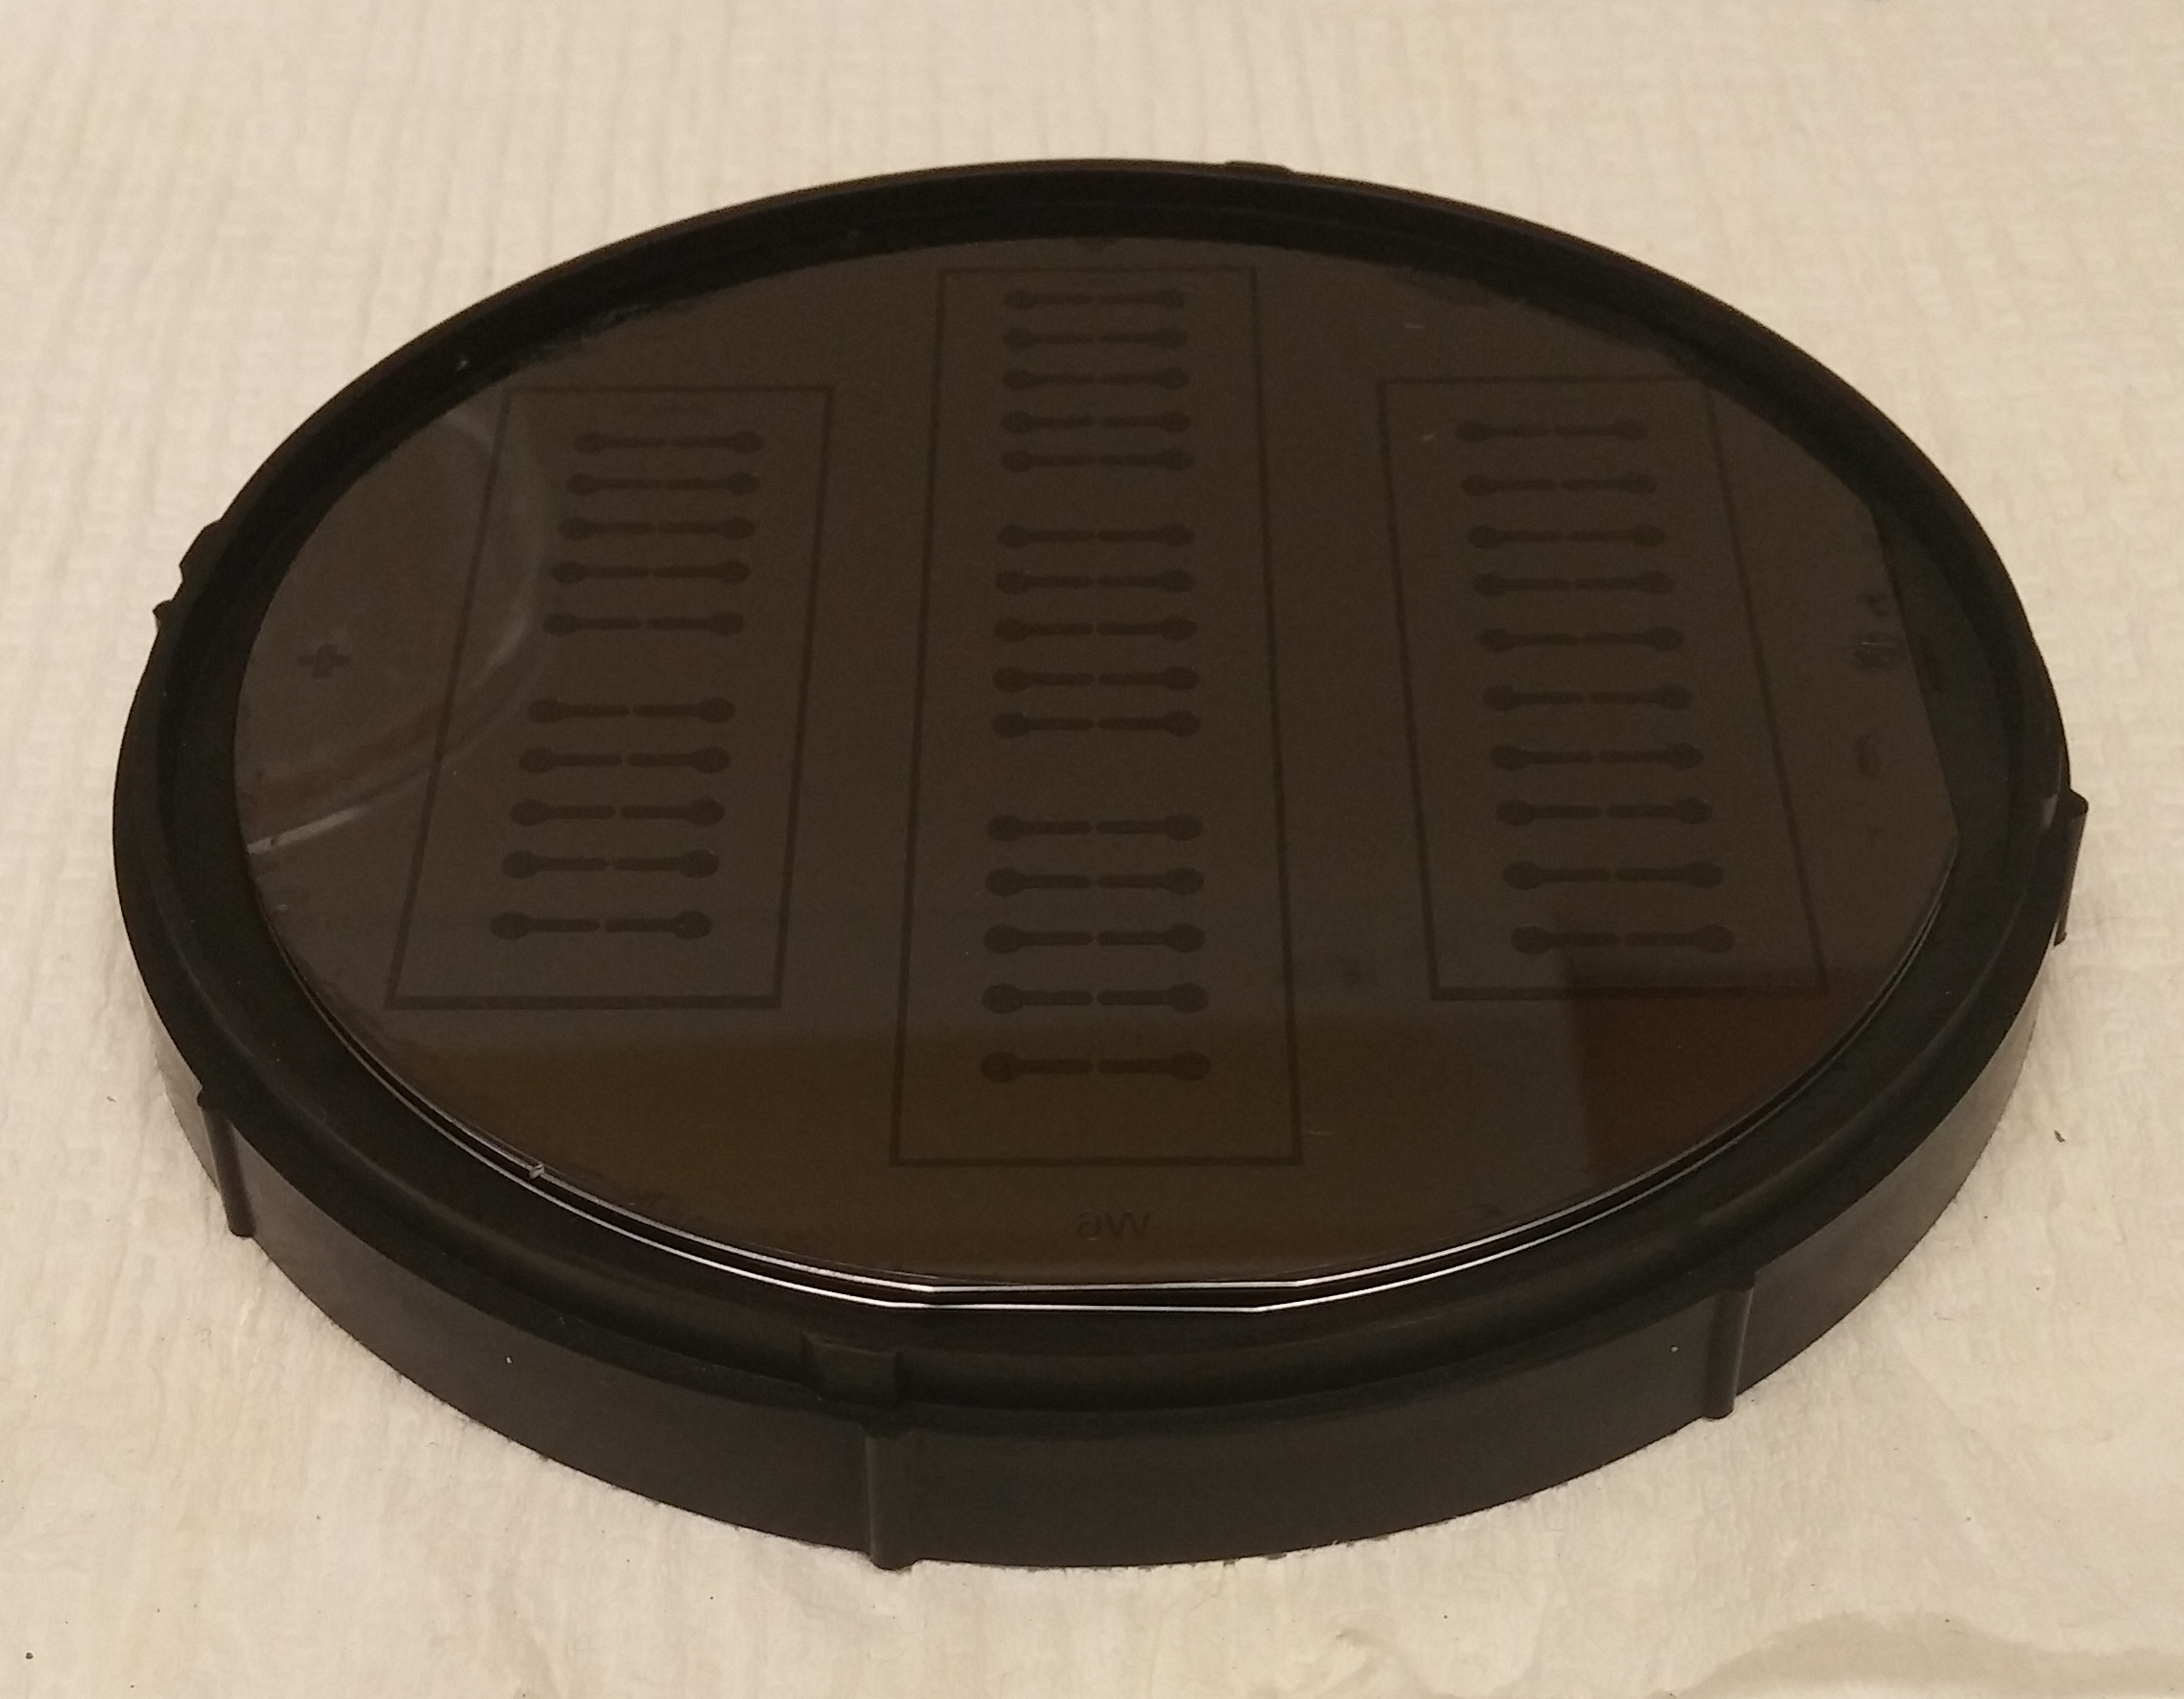
\includegraphics[height=.85in]{wafer} \\
				Silicon/SU8 wafer \\
				\par
			}
		\end{column}
		
		\begin{column}[T]{1.67in}
			{\centering
				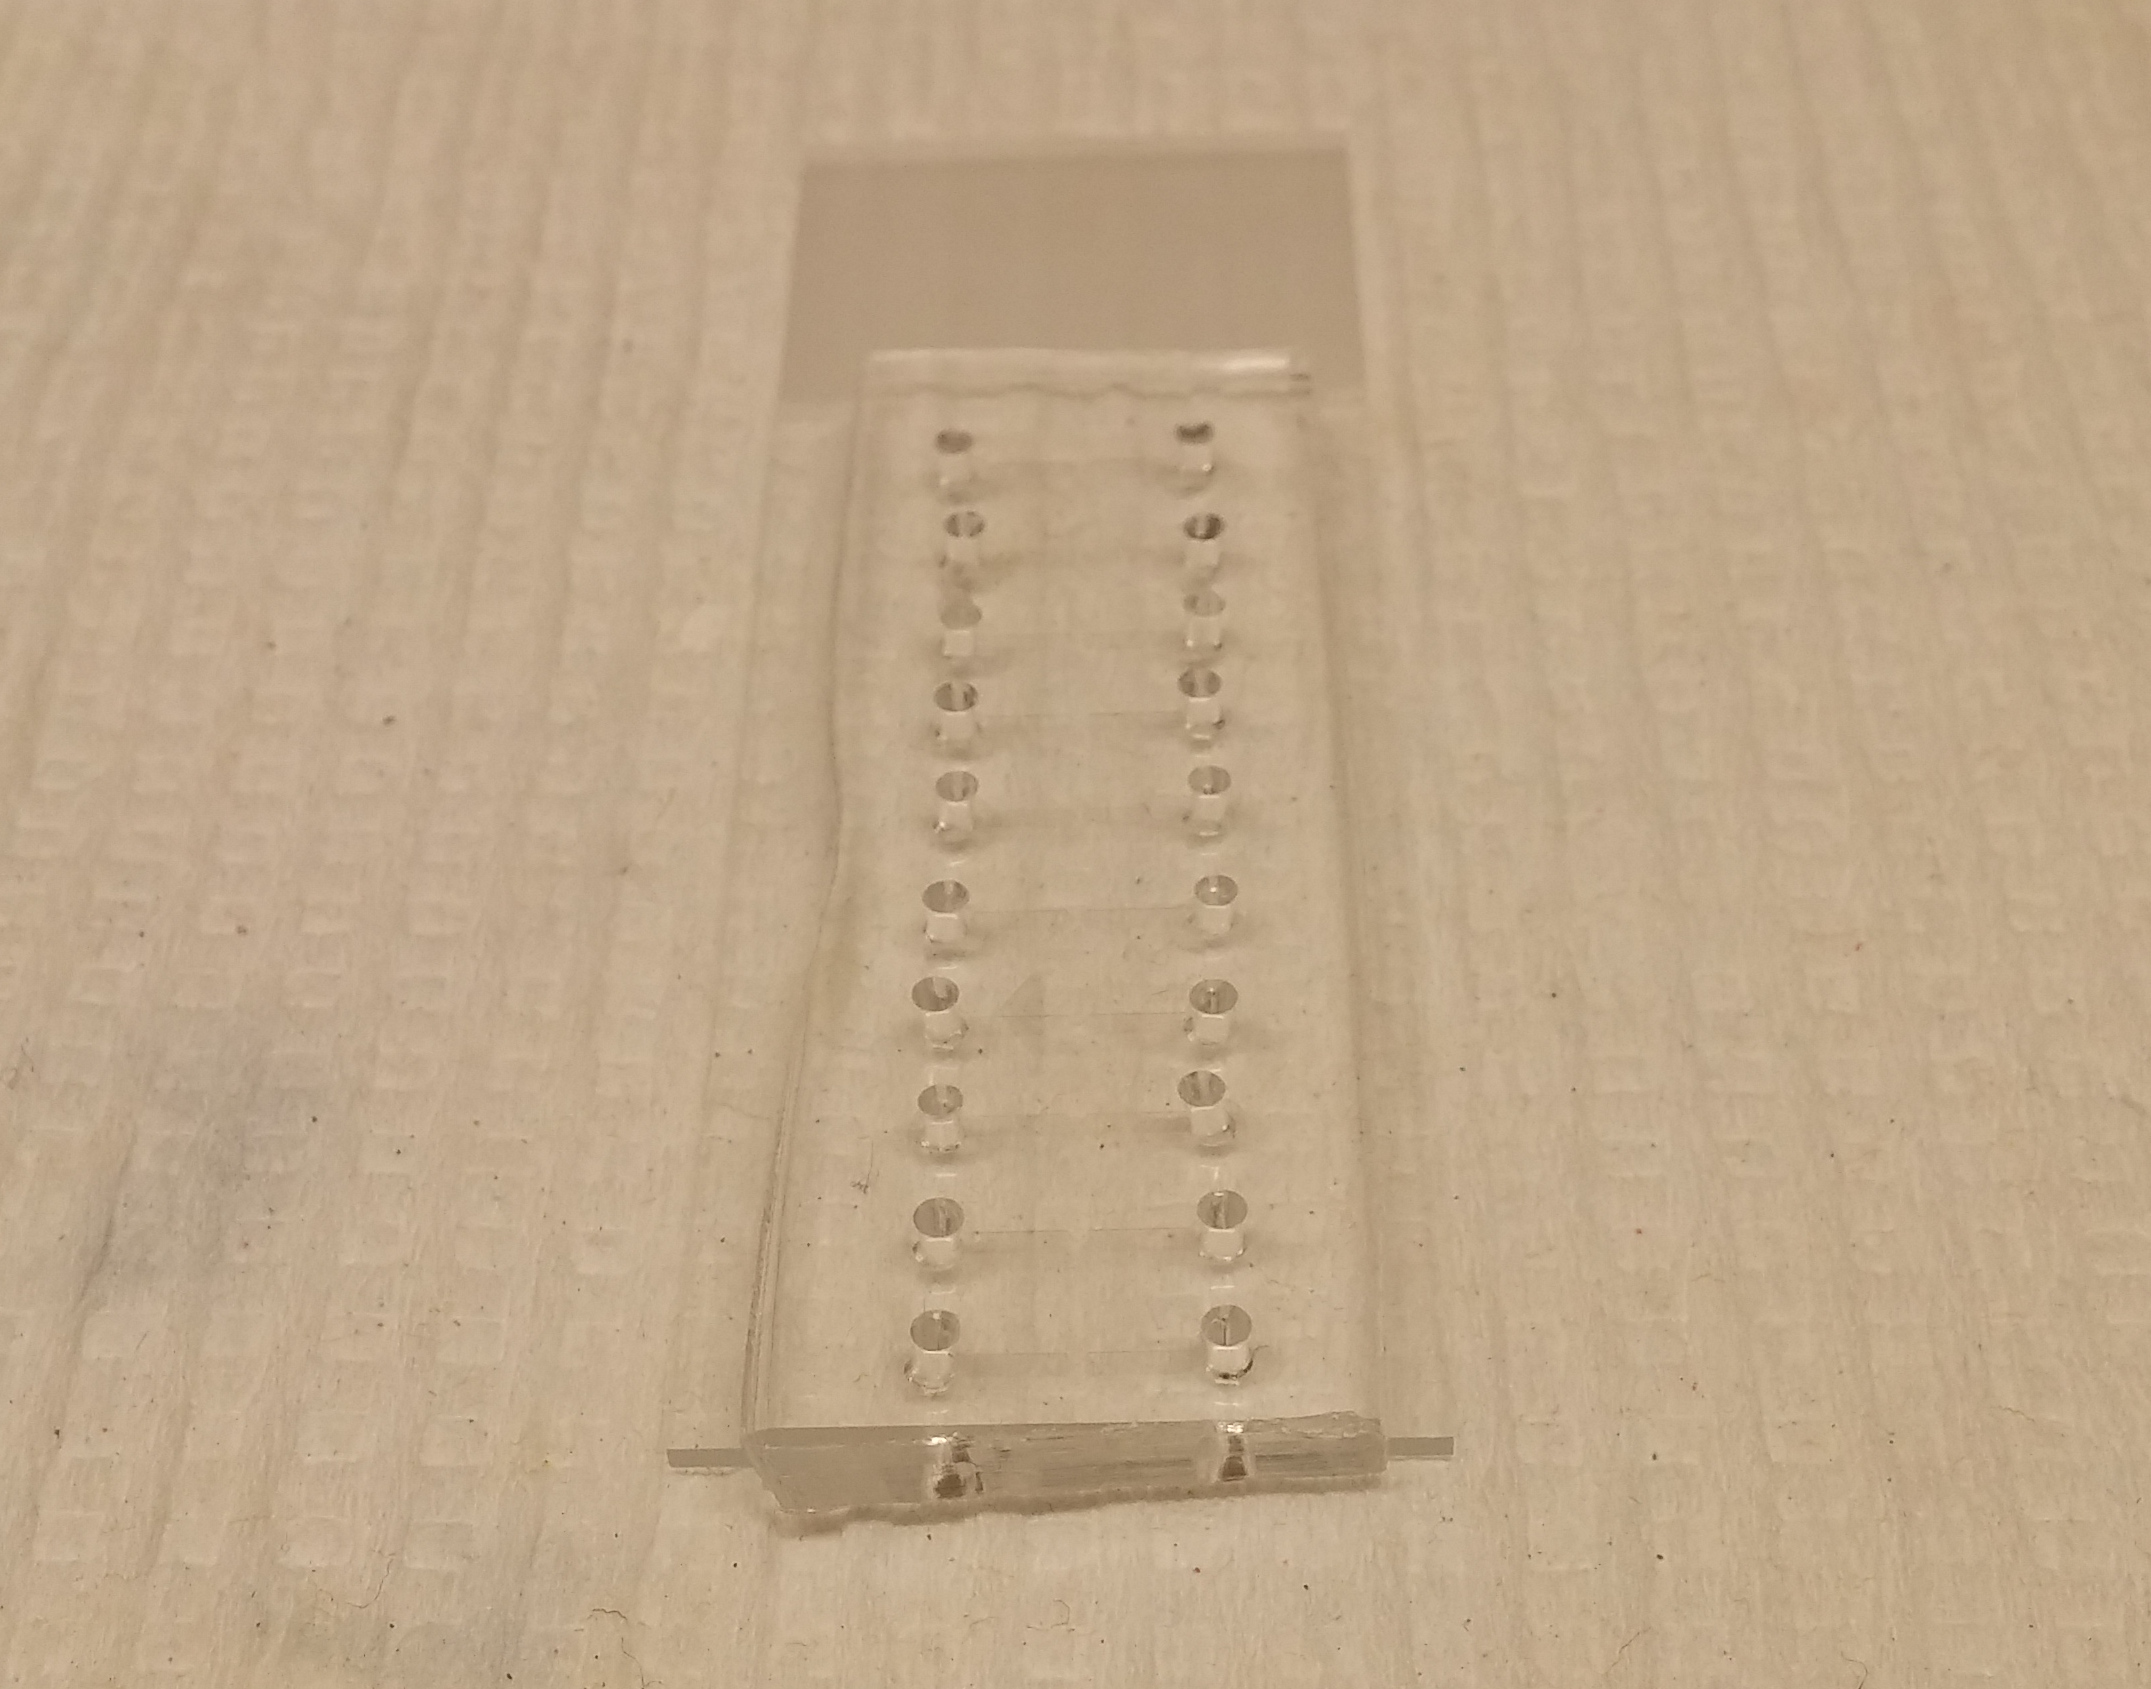
\includegraphics[height=.85in]{chip} \\
				PDMS channels
				\par
			}
		\end{column}

	\end{columns}


\end{frame}


%%%%%%%%%%%%%%%%%%%%%%%%%%%%%%%%%%%%%%%%%%%%%%%%%%%%%%%%%%%%%%%%%%%%%%%%%%%%%%%%%%%%%%%%%%%%%%%%%%%%%%%%%%%%%%%%%%%%%%%%%%%%
% Experimental set up
%%%%%%%%%%%%%%%%%%%%%%%%%%%%%%%%%%%%%%%%%%%%%%%%%%%%%%%%%%%%%%%%%%%%%%%%%%%%%%%%%%%%%%%%%%%%%%%%%%%%%%%%%%%%%%%%%%%%%%%%%%%%


\begin{frame}[c]{Hardware configuration}


	{\footnotesize
		Device is placed on the stage of a microscope, which has a high-speed camera $\left(>\SI{100}{kfps}!\right)$ attached for capturing the images \\
		\vspace{.1in}
		Electrodes are attached at the channel access ports for recording the RP signal \\
		\vspace{.1in}
		A particle suspension is driven through the channels \textit{via} syringe pump \\
		\vspace{.1in}
		The camera and resistive pulse data are simultaneously recorded \\
	}
	
	{\centering 
		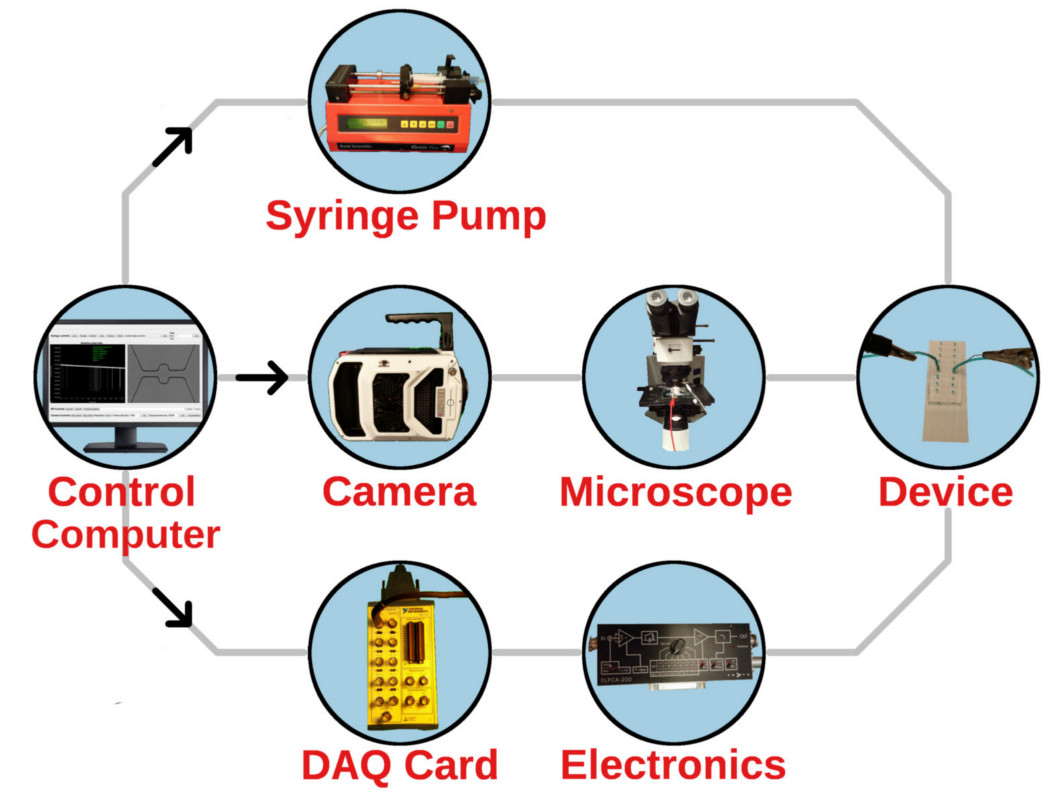
\includegraphics[width=2.5in]{hardware.jpg} \\
		\par
	}
	

\end{frame}



%%%%%%%%%%%%%%%%%%%%%%%%%%%%%%%%%%%%%%%%%%%%%%%%%%%%%%%%%%%%%%%%%%%%%%%%%%%%%%%%%%%%%%%%%%%%%%%%%%%%%%%%%%%%%%%%%%%%%%%%%%%%
% Total experimental set up
%%%%%%%%%%%%%%%%%%%%%%%%%%%%%%%%%%%%%%%%%%%%%%%%%%%%%%%%%%%%%%%%%%%%%%%%%%%%%%%%%%%%%%%%%%%%%%%%%%%%%%%%%%%%%%%%%%%%%%%%%%%%


\begin{frame}[c]{Hardware configuration}


	{\centering 
		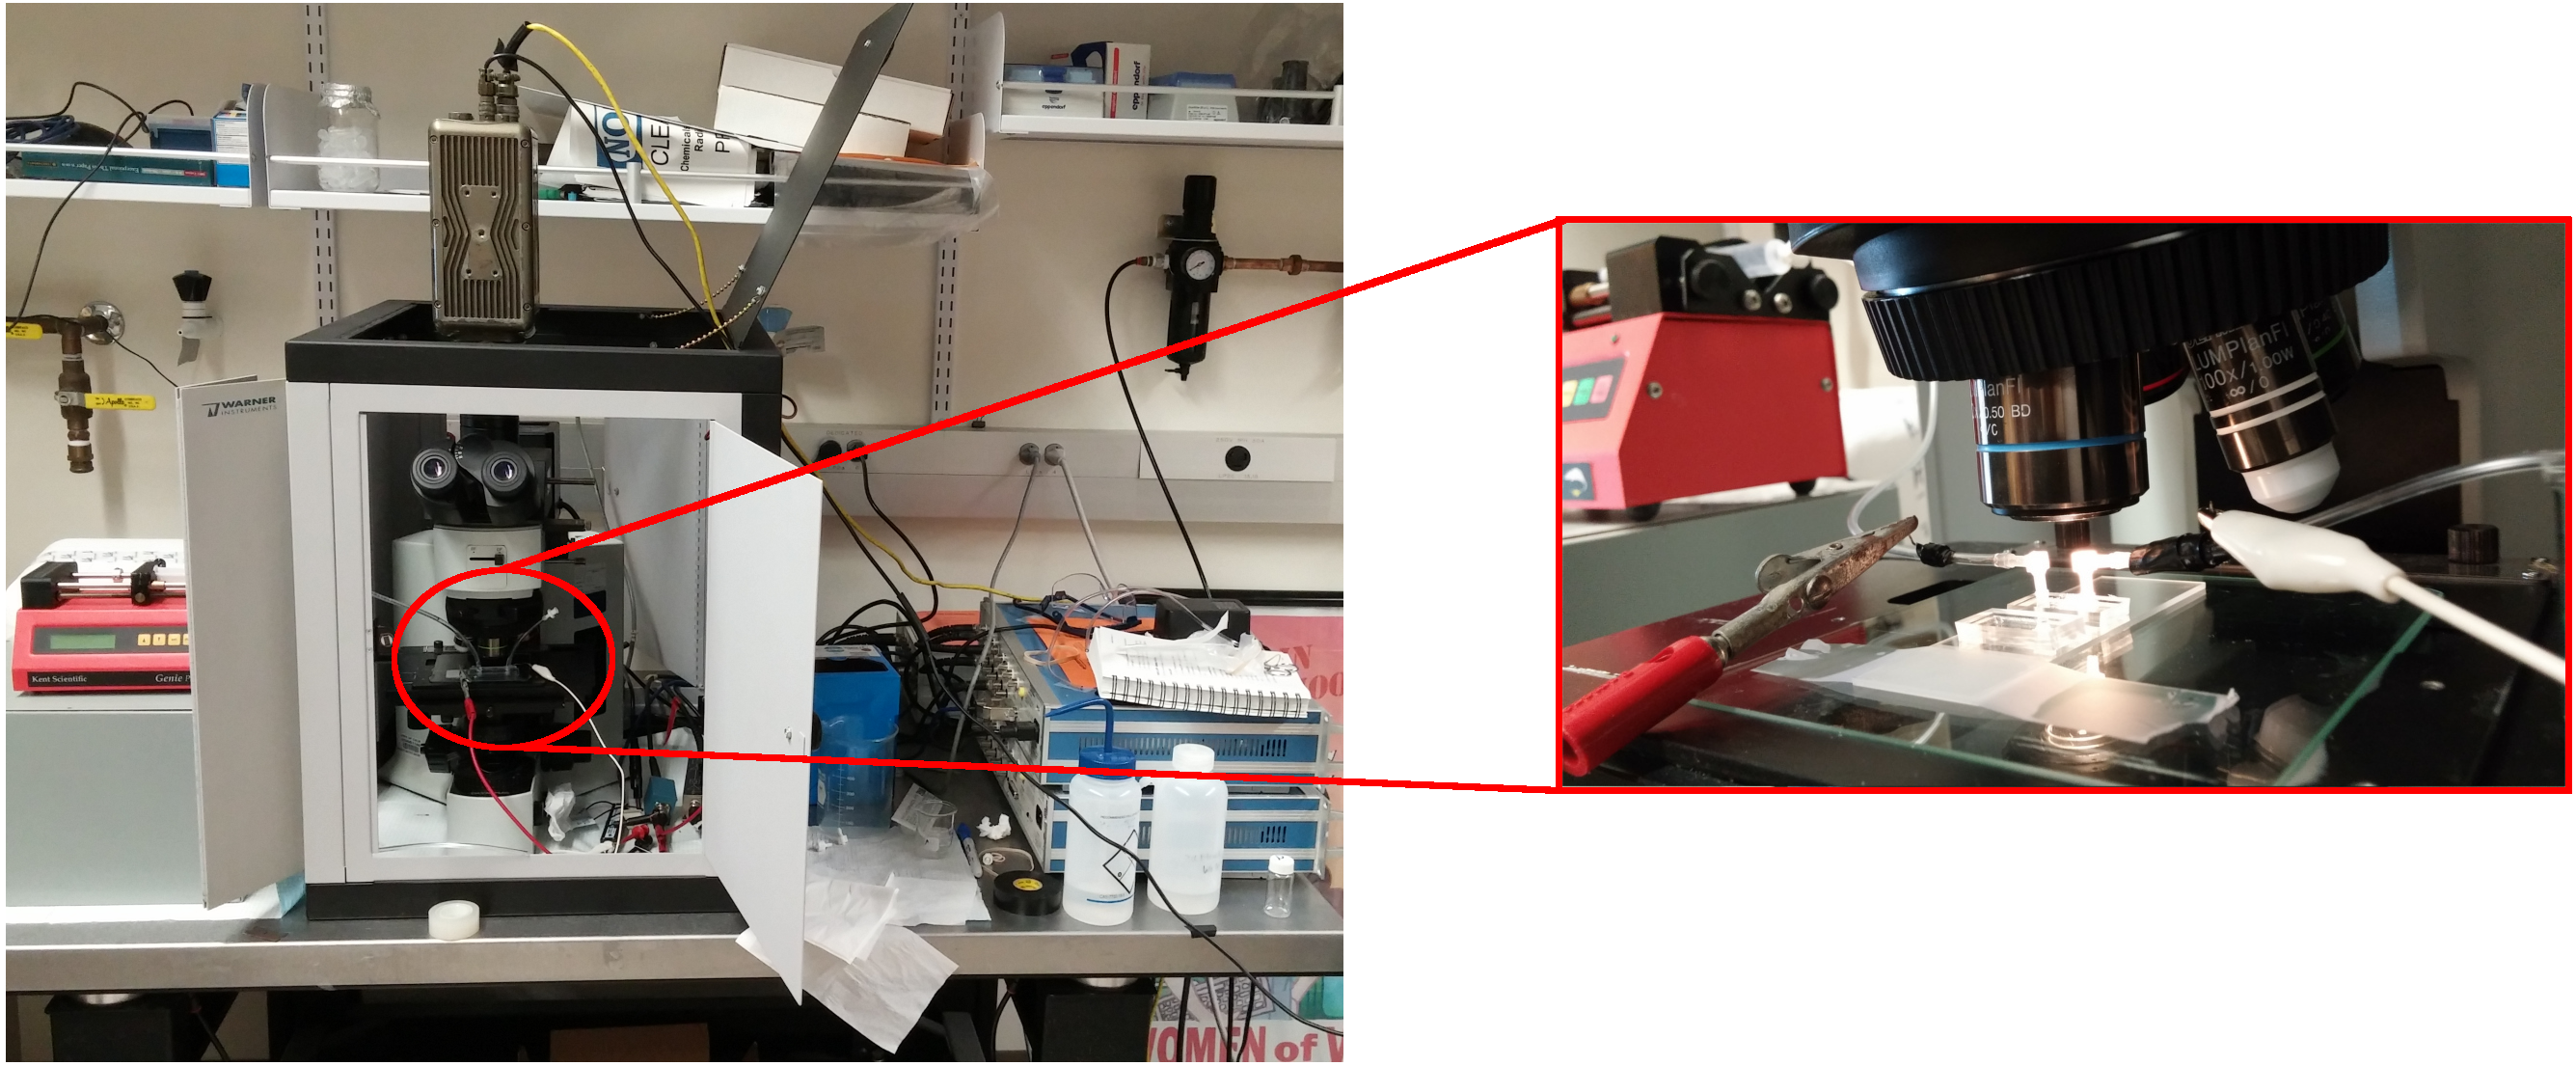
\includegraphics[width=4.5in]{setup_chip_closeup.png} \\
		\par
	}
	
	

\end{frame}



%%%%%%%%%%%%%%%%%%%%%%%%%%%%%%%%%%%%%%%%%%%%%%%%%%%%%%%%%%%%%%%%%%%%%%%%%%%%%%%%%%%%%%%%%%%%%%%%%%%%%%%%%%%%%%%%%%%%%%%%%%%%
% Channels and particles
%%%%%%%%%%%%%%%%%%%%%%%%%%%%%%%%%%%%%%%%%%%%%%%%%%%%%%%%%%%%%%%%%%%%%%%%%%%%%%%%%%%%%%%%%%%%%%%%%%%%%%%%%%%%%%%%%%%%%%%%%%%%


\begin{frame}[c]{Channels and particles}

	\begin{columns}[t]
		\begin{column}[T]{2.25in}
			{\centering 
				\includegraphics[height=1.15in]{polystyrene_bangs} \\
				$\SI{10}{\mu m}$ polystyrene beads \\
				\par
			}		 
		\end{column}
		
		\begin{column}[T]{2.25in}
			{\centering 
				\includegraphics[height=1.15in]{trajectories} \\
				PDMS channels \\
				{\footnotesize
					\textbf{Top row:} straight \\
					\textbf{Bottom row:} with cavity \\
					\par
				}
			}		 
		\end{column}
	\end{columns}	

\end{frame}



%%%%%%%%%%%%%%%%%%%%%%%%%%%%%%%%%%%%%%%%%%%%%%%%%%%%%%%%%%%%%%%%%%%%%%%%%%%%%%%%%%%%%%%%%%%%%%%%%%%%%%%%%%%%%%%%%%%%%%%%%%%%
% Raw data
%%%%%%%%%%%%%%%%%%%%%%%%%%%%%%%%%%%%%%%%%%%%%%%%%%%%%%%%%%%%%%%%%%%%%%%%%%%%%%%%%%%%%%%%%%%%%%%%%%%%%%%%%%%%%%%%%%%%%%%%%%%%


\begin{frame}[c]{Raw data---resistive pulse and optics}


	\begin{columns}[t]
		\begin{column}[T]{2.25in}
			{\centering 
				\includegraphics[height=1.25in]{rp_timeseries.png} \\
				Raw RP series \\
				data = $I\left(t\right)$ \\
				\par
			}
		\end{column}
		
		
		\begin{column}[T]{2.25in}
			{\centering 
				\includegraphics[height=1.25in]{raw_video_2.png} \\
				Image stills \\
				data = $\left\{\mathrm{frame1, frame2, ...}\right\}$
				\par
			}
		\end{column}
	\end{columns}
	\vspace{.2in}
	
	Start with two raw data streams recorded independently \\
		
	\begin{itemize}
		\item The objective is to connect the two data sets so that we know the instantaneous value of the current for each frame
		\item This will allow us to map the instanteous state of the channel (occupancy, occupant position) to the current level
	\end{itemize}



\end{frame}


%%%%%%%%%%%%%%%%%%%%%%%%%%%%%%%%%%%%%%%%%%%%%%%%%%%%%%%%%%%%%%%%%%%%%%%%%%%%%%%%%%%%%%%%%%%%%%%%%%%%%%%%%%%%%%%%%%%%%%%%%%%%
% Tracked events
%%%%%%%%%%%%%%%%%%%%%%%%%%%%%%%%%%%%%%%%%%%%%%%%%%%%%%%%%%%%%%%%%%%%%%%%%%%%%%%%%%%%%%%%%%%%%%%%%%%%%%%%%%%%%%%%%%%%%%%%%%%%


\begin{frame}[c]{Tracked events}

	\begin{columns}[t]
		\begin{column}[T]{2.25in}
			{\centering 
				\includegraphics[height=1.45in]{single_rp_event.png} \\
				data = $\frac{\Delta I}{I_{p}}\left(t_{RP}\right)$ \\
				\par
			}
		\end{column}
		
		
		\begin{column}[T]{2.25in}
			{\centering 
				\movie[height=1.25in,width=2.25in,autostart,loop]{}{trajectory_vid.mp4} \\
				\vspace{.225in}
				data = $\vec{x}_{c}\left(t_{IM}\right)$
				\par
			}
		\end{column}
	\end{columns}
	\vspace{.2in}
	
	Resistive pulse events and imaging events are independently detected in both data sets
	\begin{itemize}
		\item RP events are detected via a threshold algorithm
		\item Individual particles are detected via image processing techniques and tracked across frames
	\end{itemize}
	

\end{frame}



%%%%%%%%%%%%%%%%%%%%%%%%%%%%%%%%%%%%%%%%%%%%%%%%%%%%%%%%%%%%%%%%%%%%%%%%%%%%%%%%%%%%%%%%%%%%%%%%%%%%%%%%%%%%%%%%%%%%%%%%%%%%
% Synchronizing the two data sets
%%%%%%%%%%%%%%%%%%%%%%%%%%%%%%%%%%%%%%%%%%%%%%%%%%%%%%%%%%%%%%%%%%%%%%%%%%%%%%%%%%%%%%%%%%%%%%%%%%%%%%%%%%%%%%%%%%%%%%%%%%%%


\begin{frame}[c]{Synchronizing the two data sets}

	{\scriptsize
		After the events are detected independently, we plot a sequence of the time at which each event occurs in its own data stream \\
		Then, we align the two sequences, resulting in a synchronized data set \\
		\[ \mathrm{data} = \frac{\Delta I}{I_{p}}\left(t, x_{c}, y_{c}\right) \]
	}
	
	{\centering
		\includegraphics[width=3.25in]{synced_sequences.pdf} \\
		\vspace{.2in}
		\includegraphics[width=1.25in]{synced_event.pdf} \\
		\par
	}
	
	

\end{frame}


%%%%%%%%%%%%%%%%%%%%%%%%%%%%%%%%%%%%%%%%%%%%%%%%%%%%%%%%%%%%%%%%%%%%%%%%%%%%%%%%%%%%%%%%%%%%%%%%%%%%%%%%%%%%%%%%%%%%%%%%%%%%
% Resistance maps---process video
%%%%%%%%%%%%%%%%%%%%%%%%%%%%%%%%%%%%%%%%%%%%%%%%%%%%%%%%%%%%%%%%%%%%%%%%%%%%%%%%%%%%%%%%%%%%%%%%%%%%%%%%%%%%%%%%%%%%%%%%%%%%


\begin{frame}[c]{Resistance maps}
	
	{\scriptsize
		Synchronizing the two data streams allows us to create `resistance maps' of the channel, plots where each particle position is mapped onto the instantaneous value of the RP amplitude} \\
	{\centering
		\movie[height = 0.55 \textwidth,width = .55 \textwidth,autostart,loop]{}{resistance_map_3.mp4} \\
		\par
	}
	
\end{frame}

%%%%%%%%%%%%%%%%%%%%%%%%%%%%%%%%%%%%%%%%%%%%%%%%%%%%%%%%%%%%%%%%%%%%%%%%%%%%%%%%%%%%%%%%%%%%%%%%%%%%%%%%%%%%%%%%%%%%%%%%%%%%
% Resistance maps---final image
%%%%%%%%%%%%%%%%%%%%%%%%%%%%%%%%%%%%%%%%%%%%%%%%%%%%%%%%%%%%%%%%%%%%%%%%%%%%%%%%%%%%%%%%%%%%%%%%%%%%%%%%%%%%%%%%%%%%%%%%%%%%


\begin{frame}[c]{Resistance maps}


	{\centering
		\only<1>{\includegraphics[width=0.55\textwidth]{resistance_map_undulating.png}}
		\only<2>{\includegraphics[width=0.625\textwidth]{resistancemaps.png}} \\
		\par
	}
	
\end{frame}


%%%%%%%%%%%%%%%%%%%%%%%%%%%%%%%%%%%%%%%%%%%%%%%%%%%%%%%%%%%%%%%%%%%%%%%%%%%%%%%%%%%%%%%%%%%%%%%%%%%%%%%%%%%%%%%%%%%%%%%%%%%%
% Resistance maps---final image
%%%%%%%%%%%%%%%%%%%%%%%%%%%%%%%%%%%%%%%%%%%%%%%%%%%%%%%%%%%%%%%%%%%%%%%%%%%%%%%%%%%%%%%%%%%%%%%%%%%%%%%%%%%%%%%%%%%%%%%%%%%%


\begin{frame}[c]{Key scientific questions}
	
	The hybrid resistive pulse-imaging platform is a general tool for enhancing the interpretability of resistive pulse experiments \\
	\vspace{.1in}
	We were interested in answering the following: \\
	
	\begin{itemize}
		\item How far into a channel must a particle travel before the RP amplitude plateaus?
		\item How does off-axis translocation effect the RP amplitude in constant width and non-constant width channels?
		\item How is the resistance distributed in channels with varying widths?
	\end{itemize}
	
	
\end{frame}



%%%%%%%%%%%%%%%%%%%%%%%%%%%%%%%%%%%%%%%%%%%%%%%%%%%%%%%%%%%%%%%%%%%%%%%%%%%%%%%%%%%%%%%%%%%%%%%%%%%%%%%%%%%%%%%%%%%%%%%%%%%%
% Distance into channel
%%%%%%%%%%%%%%%%%%%%%%%%%%%%%%%%%%%%%%%%%%%%%%%%%%%%%%%%%%%%%%%%%%%%%%%%%%%%%%%%%%%%%%%%%%%%%%%%%%%%%%%%%%%%%%%%%%%%%%%%%%%%


\begin{frame}[c]{Channel entrance effects}

	{\scriptsize
		In RP experiments, event duration can be used to measure the $\zeta-$potential of the particle or pore \\
		\vspace{0.1in}
		In order to measure duration accurately, the exact time corresponding to particle entrance and exit must be known \\
		\vspace{0.1in}
		There is no standard point in RP signal at which to mark the event start and stop \\
		\vspace{0.1in}
	}
	
	\vspace{0.1in}

	\hspace{1.in} \includegraphics[width=1in]{channel_entrance_resistance_map.png} \\
	
	\begin{tikzpicture}[overlay, x=1cm,y=1cm]
		% Coordinates
		\coordinate (x1a) at (3.25, 1.35) ;
		\coordinate (x1b) at (2, -0.25) ;
		
		\coordinate (x2a) at (4, 1.35) ;
		\coordinate (x2b) at (7.05, .25) ;
		
		\coordinate (x3a) at (4.5, 1.35) ;
		\coordinate (x3b) at (6.35, 1.75) ;


		% Text hack
		\node[right] (mag) at (0.25,-0.5) {\footnotesize\textcolor{porestatsblack}{Bulk resistance}};
		\node[right] (mag) at (7.25,0.25) {\footnotesize\textcolor{porestatsblack}{Transition zone}};
		\node[right] (mag) at (6.5,1.75) {\footnotesize\textcolor{porestatsblack}{Intrachannel resistance}};


		    		    
		% Arrow
		\path[draw=gray1,thick,->] (x1a) to[bend right] (x1b) ;
		\path[draw=gray1,thick,->] (x2a) to[bend right] (x2b) ;
		\path[draw=gray1,thick,->] (x3a) to[bend left] (x3b) ;
		


			
	\end{tikzpicture}
	

	
\end{frame}




%%%%%%%%%%%%%%%%%%%%%%%%%%%%%%%%%%%%%%%%%%%%%%%%%%%%%%%%%%%%%%%%%%%%%%%%%%%%%%%%%%%%%%%%%%%%%%%%%%%%%%%%%%%%%%%%%%%%%%%%%%%%
% Distance into channel
%%%%%%%%%%%%%%%%%%%%%%%%%%%%%%%%%%%%%%%%%%%%%%%%%%%%%%%%%%%%%%%%%%%%%%%%%%%%%%%%%%%%%%%%%%%%%%%%%%%%%%%%%%%%%%%%%%%%%%%%%%%%


\begin{frame}[c]{Channel entrance effects}
	
	{\scriptsize
		Plotting current amplitude $\Delta I/I_{p}$ versus axial position $x_{c}$ shows how the current transitions to its full amplitude as the particle enters the channel \\
		\vspace{.1in}
		We found the full amplitude was not attained until the particle was well-within the channel, even as much as $\sim\SI{10}{\mu m}$ ($7\%$ of the total channel length) \\
		\vspace{.1in}
		The channel-crossing threshold most closely coincides with the FWHM of the RP signal, suggesting that current value may be the most appropriate to choose for the channel entrance and exit positions \\
	}
	
	
	{\centering
		\includegraphics[width=3in]{channelentrancestraight.pdf} \\
		\par
	}
	

	
\end{frame}


%%%%%%%%%%%%%%%%%%%%%%%%%%%%%%%%%%%%%%%%%%%%%%%%%%%%%%%%%%%%%%%%%%%%%%%%%%%%%%%%%%%%%%%%%%%%%%%%%%%%%%%%%%%%%%%%%%%%%%%%%%%%
% Effect of off-axis translocation---Introduction
%%%%%%%%%%%%%%%%%%%%%%%%%%%%%%%%%%%%%%%%%%%%%%%%%%%%%%%%%%%%%%%%%%%%%%%%%%%%%%%%%%%%%%%%%%%%%%%%%%%%%%%%%%%%%%%%%%%%%%%%%%%%


\begin{frame}[c]{Effect of off-axis translocations}
	
	{\scriptsize
		Electrostatic boundary conditions at the surface of the insulating particle leads to distortion of the electric field in its vicinity \\
		\vspace{.1in}
		{\centering
			\includegraphics[height=.65in]{channel_coordinates.pdf}
			\hspace{.4in}
			\includegraphics[height=.65in]{berge_fig.png} \\ 
			\par
		}
		
		\vspace{.1in}
		When the particle travels off-axis, this distortion couples with the distortion of the $\vec{E}$ field in the vicinity of the channel, increasing the total system resistance \\
		\vspace{.1in}
		This off-axis effect leads to a dispersion in the amplitudes produced by particles of the same size, ultimately resulting in larger uncertainties in their measured volumes \\
		\vspace{.025in}
		\begin{columns}[t]
			\begin{column}[T]{1.75in}
				\includegraphics[width=1.65in]{saleh_fig.png} \\
				{\tiny Saleh, O.A. and Sohn, L.L. \textit{Rev. Sci. Instrum.} \textbf{73}, 4396--4398 (2002).} \\ 
				\par
			\end{column}
		\end{columns}

		
	}
	
\end{frame}



%%%%%%%%%%%%%%%%%%%%%%%%%%%%%%%%%%%%%%%%%%%%%%%%%%%%%%%%%%%%%%%%%%%%%%%%%%%%%%%%%%%%%%%%%%%%%%%%%%%%%%%%%%%%%%%%%%%%%%%%%%%%
% Effect of off-axis translocation---Straight channels
%%%%%%%%%%%%%%%%%%%%%%%%%%%%%%%%%%%%%%%%%%%%%%%%%%%%%%%%%%%%%%%%%%%%%%%%%%%%%%%%%%%%%%%%%%%%%%%%%%%%%%%%%%%%%%%%%%%%%%%%%%%%


\begin{frame}[c]{Off-axis translocation in straight channels}
	
	{\centering
		\includegraphics[width=1.75in]{off_axis_straight.pdf} \\
		{\scriptsize \textcolor{negativered}{The scatter plots show an increase in event amplitude of close to 10\%, in agreement with theoretical expectations.} } \\
		\par
	}
	
\end{frame}



%%%%%%%%%%%%%%%%%%%%%%%%%%%%%%%%%%%%%%%%%%%%%%%%%%%%%%%%%%%%%%%%%%%%%%%%%%%%%%%%%%%%%%%%%%%%%%%%%%%%%%%%%%%%%%%%%%%%%%%%%%%%
% Effect of off-axis translocation---Undulating channels
%%%%%%%%%%%%%%%%%%%%%%%%%%%%%%%%%%%%%%%%%%%%%%%%%%%%%%%%%%%%%%%%%%%%%%%%%%%%%%%%%%%%%%%%%%%%%%%%%%%%%%%%%%%%%%%%%%%%%%%%%%%%


\begin{frame}[c]{Off-axis translocation in cavitated channels}
	
	{\centering
		\includegraphics[width=3.75in]{off_axis_cavity.pdf} \\
		{\scriptsize \textcolor{negativered}{In channels with a central cavity, we observe the opposite effect of lateral displacement when the particle is inside the cavity.} } \\
		\par
	}
	
\end{frame}




%%%%%%%%%%%%%%%%%%%%%%%%%%%%%%%%%%%%%%%%%%%%%%%%%%%%%%%%%%%%%%%%%%%%%%%%%%%%%%%%%%%%%%%%%%%%%%%%%%%%%%%%%%%%%%%%%%%%%%%%%%%%
% Conclusions and future work
%%%%%%%%%%%%%%%%%%%%%%%%%%%%%%%%%%%%%%%%%%%%%%%%%%%%%%%%%%%%%%%%%%%%%%%%%%%%%%%%%%%%%%%%%%%%%%%%%%%%%%%%%%%%%%%%%%%%%%%%%%%%


\begin{frame}[c]{Conclusions and ongoing work}


	{\centering
		\includegraphics[width=3in]{paper/scientificreports.png} \\
		\par
	}
	
	\vspace{.4in}
	{\small
		The hybrid resistive pulse-optical detection platform allows one to explore position-related effects on the resistive pulse amplitude \\
		\vspace{.1in}
		We are currently interested in using the hybrid approach to study particle deformation dynamics, and how deformation affects the resistive pulse amplitudes \\
	}

	
\end{frame}


%%%%%%%%%%%%%%%%%%%%%%%%%%%%%%%%%%%%%%%%%%%%%%%%%%%%%%%%%%%%%%%%%%%%%%%%%%%%%%%%%%%%%%%%%%%%%%%%%%%%%%%%%%%%%%%%%%%%%%%%%%%%
% Cell title slide
%%%%%%%%%%%%%%%%%%%%%%%%%%%%%%%%%%%%%%%%%%%%%%%%%%%%%%%%%%%%%%%%%%%%%%%%%%%%%%%%%%%%%%%%%%%%%%%%%%%%%%%%%%%%%%%%%%%%%%%%%%%%

\begin{frame}[c]{}
	\begin{center}
		\textbf{Resistive pulse sensing of biological cells}
	\end{center}
\end{frame}





%%%%%%%%%%%%%%%%%%%%%%%%%%%%%%%%%%%%%%%%%%%%%%%%%%%%%%%%%%%%%%%%%%%%%%%%%%%%%%%%%%%%%%%%%%%%%%%%%%%%%%%%%%%%%%%%%%%%%%%%%%%%
% Cell background slide
%%%%%%%%%%%%%%%%%%%%%%%%%%%%%%%%%%%%%%%%%%%%%%%%%%%%%%%%%%%%%%%%%%%%%%%%%%%%%%%%%%%%%%%%%%%%%%%%%%%%%%%%%%%%%%%%%%%%%%%%%%%%

\begin{frame}[c]{Cell mechanical properties}
	\begin{columns}[t]
		\begin{column}[T]{2.25in}
			\begin{itemize}
				\item Traditional cell characterization platforms have been primarily chemical,~e.g. fluorescence microscopy
				\item Recently, researchers have recognized the importance of measuring mechanical properties of cells
				\item For instance, size and shape can be predictive of cell type
			\end{itemize}
		\end{column}
		
		
		\begin{column}[T]{2.25in}
			\includegraphics[width=2.25in]{bloodcells.jpg}
		\end{column}


	\end{columns}

	

\end{frame}



%%%%%%%%%%%%%%%%%%%%%%%%%%%%%%%%%%%%%%%%%%%%%%%%%%%%%%%%%%%%%%%%%%%%%%%%%%%%%%%%%%%%%%%%%%%%%%%%%%%%%%%%%%%%%%%%%%%%%%%%%%%%
% Cell background slide
%%%%%%%%%%%%%%%%%%%%%%%%%%%%%%%%%%%%%%%%%%%%%%%%%%%%%%%%%%%%%%%%%%%%%%%%%%%%%%%%%%%%%%%%%%%%%%%%%%%%%%%%%%%%%%%%%%%%%%%%%%%%

\begin{frame}[c]{Cell mechanical properties}
	\begin{itemize}
		\item Another important mechanical feature is stiffness---cells are elastic and deformable objects
		\item Stiffness depends on physiological properties in the membrane and body, such as cytoskeletal strength
		\item Stiffness varies across cell lines, and has shown to be predictive in the same way as size and shape are---for instance, cancer cells are generally more elastic than non-cancerous cells
		
	\end{itemize}

\end{frame}


%%%%%%%%%%%%%%%%%%%%%%%%%%%%%%%%%%%%%%%%%%%%%%%%%%%%%%%%%%%%%%%%%%%%%%%%%%%%%%%%%%%%%%%%%%%%%%%%%%%%%%%%%%%%%%%%%%%%%%%%%%%%
% Cell background slide
%%%%%%%%%%%%%%%%%%%%%%%%%%%%%%%%%%%%%%%%%%%%%%%%%%%%%%%%%%%%%%%%%%%%%%%%%%%%%%%%%%%%%%%%%%%%%%%%%%%%%%%%%%%%%%%%%%%%%%%%%%%%

\begin{frame}[c]{Stiffness detection}

	\begin{itemize}
		\item Is it possible to build a sensor that measures cell deformability?
		\item One way to measure deformability is to drive cells through ultra fast fluidic flows
		\item Hydrodynamic forces act on the particle, inducing a measurable deformation response
	\end{itemize}
	
	\vspace{.1in}
	
	{\centering
		\includegraphics[width=3in]{otto_et_al.png} \\
		{\tiny Otto \textit{et al.} \textit{Biophys. J.} \textbf{109}, 2023--2036 (2015).} \\
		\par
	}
	
	
% 	{\centering
% 		\only<1>{\includegraphics[width=3in]{otto_et_al.png}}\only<2>{\includegraphics[width=2in]{dicarlo_et_al.png}} \\
% 		{\tiny \only<1>{Otto \emph{et al.} \textit{Biophys. J.} 
% 		\textbf{109}, 2023--2036 (2015).}\only<2>{Gossett \emph{et al.} \textit{Proc. Natl. Acad. Sci. USA} \textbf{109}, 7630--7635 (2012).}} \\
% 		\par
% 	}
\end{frame}


%%%%%%%%%%%%%%%%%%%%%%%%%%%%%%%%%%%%%%%%%%%%%%%%%%%%%%%%%%%%%%%%%%%%%%%%%%%%%%%%%%%%%%%%%%%%%%%%%%%%%%%%%%%%%%%%%%%%%%%%%%%%
% Optical response measurement
%%%%%%%%%%%%%%%%%%%%%%%%%%%%%%%%%%%%%%%%%%%%%%%%%%%%%%%%%%%%%%%%%%%%%%%%%%%%%%%%%%%%%%%%%%%%%%%%%%%%%%%%%%%%%%%%%%%%%%%%%%%%

\begin{frame}[c]{Optical measurement of deformation}
	\begin{itemize}
		\item The cell's deformation response is usually determined via high-speed microscopy \\
		\item High-speed imaging is computationally expensive---many images must be rapidly recorded and undergo complex transformations in order to fit the shape of each cell \\
		\item Real-time analysis is bottlenecked at the CPU; current throughputs are only $\sim100$ cells/second \\
		\item Can we replace imaging with resistive pulse, which is less computationally demanding to analyze?
	\end{itemize}
	
	Imaging bandwidth $\sim\SI{1}{GB/s}$ \\
	Resistive pulse bandwidth $\sim\SI{1}{MB/s}$
\end{frame}


%%%%%%%%%%%%%%%%%%%%%%%%%%%%%%%%%%%%%%%%%%%%%%%%%%%%%%%%%%%%%%%%%%%%%%%%%%%%%%%%%%%%%%%%%%%%%%%%%%%%%%%%%%%%%%%%%%%%%%%%%%%%
% Measuring deformability with resistive pulse
%%%%%%%%%%%%%%%%%%%%%%%%%%%%%%%%%%%%%%%%%%%%%%%%%%%%%%%%%%%%%%%%%%%%%%%%%%%%%%%%%%%%%%%%%%%%%%%%%%%%%%%%%%%%%%%%%%%%%%%%%%%%

\begin{frame}[c]{Optical measurement of deformation}

	{\scriptsize
		We can approximate deformed cell configurations as ellipsoids, which have resistive pulse amplitude described by \\
		
		\[ \frac{\Delta I}{I_{p}}=f_{\parallel}\frac{v}{V} \] \\
		
		$f_{\parallel}$: `electrical shape factor', related to aspect ratio of the ellipse \\
	}

	\vspace{.1in}
	
	{\centering
		\includegraphics[width=2.in]{dIellipsoid.png} \\
		\par
	}
	
	\vspace{.1in}
	
	Particles of the same volume but different aspect ratio have different resistive pulse amplitudes $\Delta I/I_{p}$!
	
	
\end{frame}

%%%%%%%%%%%%%%%%%%%%%%%%%%%%%%%%%%%%%%%%%%%%%%%%%%%%%%%%%%%%%%%%%%%%%%%%%%%%%%%%%%%%%%%%%%%%%%%%%%%%%%%%%%%%%%%%%%%%%%%%%%%%
% Measuring deformability with resistive pulse
%%%%%%%%%%%%%%%%%%%%%%%%%%%%%%%%%%%%%%%%%%%%%%%%%%%%%%%%%%%%%%%%%%%%%%%%%%%%%%%%%%%%%%%%%%%%%%%%%%%%%%%%%%%%%%%%%%%%%%%%%%%%

\begin{frame}[c]{Proposed channel design for inducing deformation}

	{\scriptsize
		Consider channels containing a central cavity \\
		\vspace{.1in}
		Incompressibility of the fluid means that it must slow down in the cavity \\
		\vspace{.1in}
		Accelerating extensional flows pull the particle into an elongated geometry \\
		\vspace{.1in}
		Decelerating flows compress the particle axially \\
		\vspace{.1in}
	}
	
	
	{\centering
		\includegraphics[width=4.in]{deformation_motif.png} \\
		\par
	}
			

\end{frame}


%%%%%%%%%%%%%%%%%%%%%%%%%%%%%%%%%%%%%%%%%%%%%%%%%%%%%%%%%%%%%%%%%%%%%%%%%%%%%%%%%%%%%%%%%%%%%%%%%%%%%%%%%%%%%%%%%%%%%%%%%%%%
% Measuring deformability with resistive pulse
%%%%%%%%%%%%%%%%%%%%%%%%%%%%%%%%%%%%%%%%%%%%%%%%%%%%%%%%%%%%%%%%%%%%%%%%%%%%%%%%%%%%%%%%%%%%%%%%%%%%%%%%%%%%%%%%%%%%%%%%%%%%

\begin{frame}[c]{Deformation motif in channels with central cavities}

		\begin{columns}[t]
			\begin{column}[T]{2.25in}
				According to the deformation motif presented in the previous slide, deformations should adhere to the following pattern as the particle translocates \\
				
				\begin{equation*}
					\begin{split}
						&s\rightarrow p\rightarrow o\rightarrow p\rightarrow o\rightarrow s \\
						&s: \mathrm{spherical},\,p: \mathrm{prolate},\,o:\mathrm{oblate}
					\end{split}
				\end{equation*}
				
			\end{column}


			\begin{column}[T]{2.25in}
				{\centering
					\includegraphics[width=2.25in]{dIellipsoid.png} \\
					\par
				}
			\end{column}
		
	\end{columns}
			

\end{frame}


%%%%%%%%%%%%%%%%%%%%%%%%%%%%%%%%%%%%%%%%%%%%%%%%%%%%%%%%%%%%%%%%%%%%%%%%%%%%%%%%%%%%%%%%%%%%%%%%%%%%%%%%%%%%%%%%%%%%%%%%%%%%
% Measuring deformability with resistive pulse
%%%%%%%%%%%%%%%%%%%%%%%%%%%%%%%%%%%%%%%%%%%%%%%%%%%%%%%%%%%%%%%%%%%%%%%%%%%%%%%%%%%%%%%%%%%%%%%%%%%%%%%%%%%%%%%%%%%%%%%%%%%%

\begin{frame}[c]{Resistive pulse distortion}

	{\centering
		\includegraphics[height=1.35in]{dIellipsoid.png} \\
		\vspace{0.1in}
		\includegraphics[height=1.75in]{deformation_motif_rp.png} \\
		\par
	}


\end{frame}



%%%%%%%%%%%%%%%%%%%%%%%%%%%%%%%%%%%%%%%%%%%%%%%%%%%%%%%%%%%%%%%%%%%%%%%%%%%%%%%%%%%%%%%%%%%%%%%%%%%%%%%%%%%%%%%%%%%%%%%%%%%%
% Key scientific questions
%%%%%%%%%%%%%%%%%%%%%%%%%%%%%%%%%%%%%%%%%%%%%%%%%%%%%%%%%%%%%%%%%%%%%%%%%%%%%%%%%%%%%%%%%%%%%%%%%%%%%%%%%%%%%%%%%%%%%%%%%%%%

\begin{frame}[c]{Key scientific questions}
	  
	Experiments must be conducted to answer the following questions
	\begin{enumerate}
		\item Do the cells deform according to the presented motif?
		\item Is the deformation observable in the resistive pulse signal?
	\end{enumerate}

	\vspace{.2in}
	
	The hybrid RP-IM system is employed to characterize the device and the cells' resistive pulses \\
	\vspace{0.1in}
	Ultimately, the goal is to remove the camera from the set up and measure deformability with resistive pulse alone \\
	

	
\end{frame}



%%%%%%%%%%%%%%%%%%%%%%%%%%%%%%%%%%%%%%%%%%%%%%%%%%%%%%%%%%%%%%%%%%%%%%%%%%%%%%%%%%%%%%%%%%%%%%%%%%%%%%%%%%%%%%%%%%%%%%%%%%%%
% Cell experimental set up
%%%%%%%%%%%%%%%%%%%%%%%%%%%%%%%%%%%%%%%%%%%%%%%%%%%%%%%%%%%%%%%%%%%%%%%%%%%%%%%%%%%%%%%%%%%%%%%%%%%%%%%%%%%%%%%%%%%%%%%%%%%%

\begin{frame}[c]{Experimental set up}

	Experiments were conducted with the hybrid resistive pulse-optical characterization platform \\
	Two cell lines are currently being tested \\
	\begin{enumerate}
		\item HCT-116, colorectal cancer cells (left)
		\item 293-T, embryonic kidney cells (right)
	\end{enumerate}
	
	\begin{columns}[t]
		
		\begin{column}[T]{2.25in}
			{\centering
				\includegraphics[width=1.75in]{HCT.jpg} \\
				\par
			}
		\end{column}
		
		\begin{column}[T]{2.25in}
			{\centering
				\includegraphics[width=1.75in]{293.jpg} \\
				\par
			}
		\end{column}

	\end{columns}

	
	
	

	
\end{frame}

%%%%%%%%%%%%%%%%%%%%%%%%%%%%%%%%%%%%%%%%%%%%%%%%%%%%%%%%%%%%%%%%%%%%%%%%%%%%%%%%%%%%%%%%%%%%%%%%%%%%%%%%%%%%%%%%%%%%%%%%%%%%
% Cell experimental set up
%%%%%%%%%%%%%%%%%%%%%%%%%%%%%%%%%%%%%%%%%%%%%%%%%%%%%%%%%%%%%%%%%%%%%%%%%%%%%%%%%%%%%%%%%%%%%%%%%%%%%%%%%%%%%%%%%%%%%%%%%%%%

\begin{frame}[c]{Data analysis}

	Individual cells were detected and tracked as they passed through the camera's field of view \\
	To determine whether particles deform, we fit ellipses to their borders at every frame in the video \\
	After fitting the ellipses, we have a time-series of position $\vec{x}_{c}$, and ellipse axes $\vec{a}$ and $\vec{b}$ for each frame and each particle
	
	\includegraphics[width=4.5in]{ellipse_fit.png}
	
\end{frame}

%%%%%%%%%%%%%%%%%%%%%%%%%%%%%%%%%%%%%%%%%%%%%%%%%%%%%%%%%%%%%%%%%%%%%%%%%%%%%%%%%%%%%%%%%%%%%%%%%%%%%%%%%%%%%%%%%%%%%%%%%%%%
% Do the cells deform?
%%%%%%%%%%%%%%%%%%%%%%%%%%%%%%%%%%%%%%%%%%%%%%%%%%%%%%%%%%%%%%%%%%%%%%%%%%%%%%%%%%%%%%%%%%%%%%%%%%%%%%%%%%%%%%%%%%%%%%%%%%%%

\begin{frame}[c]{Do the cells deform?}

	{\centering
		\movie[height=1.25in,width=2.25in,autostart,loop]{}{cell_deformation.mp4} \\
		\par
	}

	
\end{frame}



%%%%%%%%%%%%%%%%%%%%%%%%%%%%%%%%%%%%%%%%%%%%%%%%%%%%%%%%%%%%%%%%%%%%%%%%%%%%%%%%%%%%%%%%%%%%%%%%%%%%%%%%%%%%%%%%%%%%%%%%%%%%
% Do the cells deform?
%%%%%%%%%%%%%%%%%%%%%%%%%%%%%%%%%%%%%%%%%%%%%%%%%%%%%%%%%%%%%%%%%%%%%%%%%%%%%%%%%%%%%%%%%%%%%%%%%%%%%%%%%%%%%%%%%%%%%%%%%%%%

\begin{frame}[c]{Axial position versus aspect ratio}
	
	\begin{columns}[t]
	 
	\begin{column}[T]{2.25in}
		{\centering
			\includegraphics[width=2.25in]{position-aspect.png} \\
			\par
		}
	\end{column}
	
	
	\begin{column}[T]{2.25in}
		{\centering
			\includegraphics[width=2.25in]{dIellipsoidexpected.png} \\
			\par
		}
	\end{column}
	
	
	
	\end{columns}
	
	
	The change in the aspect ratios agrees with the motif presented for the cavitated channels \\
	
	

	
\end{frame}


%%%%%%%%%%%%%%%%%%%%%%%%%%%%%%%%%%%%%%%%%%%%%%%%%%%%%%%%%%%%%%%%%%%%%%%%%%%%%%%%%%%%%%%%%%%%%%%%%%%%%%%%%%%%%%%%%%%%%%%%%%%%
% Conclusions and future work
%%%%%%%%%%%%%%%%%%%%%%%%%%%%%%%%%%%%%%%%%%%%%%%%%%%%%%%%%%%%%%%%%%%%%%%%%%%%%%%%%%%%%%%%%%%%%%%%%%%%%%%%%%%%%%%%%%%%%%%%%%%%

\begin{frame}[c]{Conclusions and future work}
	
	We've convincingly shown that our channel configuration is inducing two modes of deformations in cells \\
	
	\vspace{.2in}
	
	Current efforts are focused on improving our optical measurement set up \\
	
	\vspace{.2in}
	
	The magnitude of deformation observed implies that cell shape changes may be detectable with resistive pulse sensing after improving the signal-to-noise of our measurements \\
	

	
\end{frame}




%%%%%%%%%%%%%%%%%%%%%%%%%%%%%%%%%%%%%%%%%%%%%%%%%%%%%%%%%%%%%%%%%%%%%%%%%%%%%%%%%%%%%%%%%%%%%%%%%%%%%%%%%%%%%%%%%%%%%%%%%%%%
% Conclusions
%%%%%%%%%%%%%%%%%%%%%%%%%%%%%%%%%%%%%%%%%%%%%%%%%%%%%%%%%%%%%%%%%%%%%%%%%%%%%%%%%%%%%%%%%%%%%%%%%%%%%%%%%%%%%%%%%%%%%%%%%%%%

\begin{frame}[c]{}

	\centering{\textbf{Thank you for your attention!}}

	
\end{frame}






%%%%%%%%%%%%%%%%%%%%%%%%%%%%%%%%%%%%%%%%%%%%%%%%%%%%%%%%%%%%%%%%%%%%%%%%%%%%%%%%%%%%%%%%%%%%%%%%%%%%%%%%%%%%%%%%%%%%%%%%%%%%
% Group
%%%%%%%%%%%%%%%%%%%%%%%%%%%%%%%%%%%%%%%%%%%%%%%%%%%%%%%%%%%%%%%%%%%%%%%%%%%%%%%%%%%%%%%%%%%%%%%%%%%%%%%%%%%%%%%%%%%%%%%%%%%%

\begin{frame}[c]{}
	
	{\centering
		{\Large \textcolor{uciblue0}{\textbf{The Siwy Lab}}} \\
		\par
	}
	
	\vspace{-.3in}
	
	\begin{columns}[t]
		
		
		\begin{column}[T]{3.5in}
			
			\vspace{.35in}
			
			\begin{columns}[t]
				\begin{column}[T]{1in}
					{\centering
						\includegraphics[height=.9in]{lab/siwy} \\
						\vspace{-.1in}
						{\tiny Prof. Zuzanna S. Siwy} \\
						\par
					}
				\end{column}
			
				\begin{column}[T]{1in}
					% Elif
					{\centering
						\includegraphics[height=.9in]{lab/elif.JPG} \\
						\vspace{-.1in}
						{\tiny Dr. Elif T{\"u}rker Acar} \\
						\par
					}
				\end{column}
			
				\begin{column}[T]{1in}
					% Yinghua
					{\centering
						\includegraphics[height=.9in]{lab/yinghua.png} \\
						\vspace{-.1in}
						{\tiny Dr. Yinghua Qiu} \\
						\par
					}
				\end{column}
			
				\begin{column}[T]{1in}
					% Tim
					{\centering
						\includegraphics[height=.9in]{lab/tim.png} \\
						\vspace{-.1in}
						{\tiny Dr. Timothy Plett} \\
						\par
					}
				\end{column}
				
				
				
				
			\end{columns}
			
			\vspace{.1in}
			
			\begin{columns}[t]
			
				\begin{column}[T]{1in}
					% Crystal
					{\centering
						\includegraphics[height=.9in]{lab/crystay.png} \\
						\vspace{-.1in}
						{\tiny Crystal Yang} \\
						\par
					}
				\end{column}
			
				\begin{column}[T]{1in}
					% Scottie
					{\centering
						\includegraphics[height=.9in]{lab/scottie.jpg} \\
						\vspace{-.1in}
						{\tiny Chih-Yuan ``Scottie'' Lin} \\
						\par
					}
				\end{column}
			
				\begin{column}[T]{1in}
					% James
					{\centering
						\includegraphics[height=.9in]{lab/james.jpg} \\
						\vspace{-.1in}
						{\tiny James Boyd} \\
						\par
					}
				\end{column}
			
				\begin{column}[T]{1in}
					% Joseph
					{\centering
						\includegraphics[height=.9in]{lab/joseph.jpg} \\
						\vspace{-.1in}
						{\tiny Joseph Martinez} \\
						\par
					}
				\end{column}
				
				
			\end{columns}
			
			\vspace{.1in}
			
			\begin{columns}[t]
				
				\begin{column}[T]{1in}
					% Cody
					{\centering
						\includegraphics[height=.9in]{lab/cody.png} \\
						\vspace{-.1in}
						{\tiny Cody Combs} \\
						\par
					}
				\end{column}
			
			
				\begin{column}[T]{1in}
					% Rachel
					{\centering
						\includegraphics[height=.9in]{lab/rachel.png} \\
						\vspace{-.1in}
						{\tiny Rachel Lucas} \\
						\par
					}
				\end{column}
			
				\begin{column}[T]{1in}
					% Freida
					{\centering
						\includegraphics[height=.9in]{lab/freida.JPG} \\
						\vspace{-.1in}
						{\tiny Freida Rivera} \\
						\par
					}
				\end{column}
			
				\begin{column}[T]{1in}
					% Aaron
					{\centering
						\includegraphics[height=.9in]{lab/aaron.JPG} \\
						\vspace{-.1in}
						{\tiny Aaron Ellis} \\
						\par
					}
				\end{column}
				
				
			\end{columns}
		\end{column}


	\end{columns}

	
	
\end{frame}


%%%%%%%%%%%%%%%%%%%%%%%%%%%%%%%%%%%%%%%%%%%%%%%%%%%%%%%%%%%%%%%%%%%%%%%%%%%%%%%%%%%%%%%%%%%%%%%%%%%%%%%%%%%%%%%%%%%%%%%%%%%%
% Acknowledgements
%%%%%%%%%%%%%%%%%%%%%%%%%%%%%%%%%%%%%%%%%%%%%%%%%%%%%%%%%%%%%%%%%%%%%%%%%%%%%%%%%%%%%%%%%%%%%%%%%%%%%%%%%%%%%%%%%%%%%%%%%%%%

\begin{frame}[c]{Acknowledgements}
	
	\underline{Dr Trisha Westerhof}---Providing cells for the experiments \\
	\vspace{.15in}
	\underline{David J. Mallin} and \underline{Matthew L. Wallace}---Camera and lighting hardware support \\
	\vspace{.15in}
	\underline{Alexandra Perebikovsky}---Photolithography training \\
	\vspace{.35in}
	
	{\centering
		{\large Beall's foundation} \\
		\vspace{0.3in}
		\includegraphics[width=2in]{lab/dsi.png} \\
		\par
	}
	
	
\end{frame}








